% =============================================================================
% TESIS DE PREGRADO - INGENIERIA CIVIL EN INFORMATICA
% Universidad Austral de Chile
%
% Titulo: Integracion de Datos y Resiliencia Comunitaria en la Dimension
%         Sociocomunitaria
%
% Autor: Esteban Nicolas Tejeda Webar
% Profesor Patrocinante: Cristian Olivares-Rodriguez
% =============================================================================

\documentclass[12pt,letterpaper,oneside]{report}

% --- Paquetes ---
\usepackage{fontspec}
% La pauta exige Times New Roman (texto) y Courier (codigo). Ambas son fuentes
% propietarias de Microsoft y no estan disponibles en Linux ni en las imagenes
% de TeX Live, por lo que se usan como respaldo las clones libres de TeX Gyre,
% metricamente identicas: Termes (Times) y Cursor (Courier).
\IfFontExistsTF{Times New Roman}
  {\setmainfont{Times New Roman}}
  {\setmainfont{TeX Gyre Termes}}
\IfFontExistsTF{Courier New}
  {\setmonofont[Scale=0.83]{Courier New}}
  {\setmonofont[Scale=0.83]{TeX Gyre Cursor}}
\usepackage[spanish]{babel}
\usepackage[letterpaper,
            top=2.5cm,
            bottom=3cm,
            left=4cm,
            right=2.5cm]{geometry}
\usepackage{setspace}              % Interlineado
\usepackage{titlesec}              % Formato de titulos
\usepackage{graphicx}
\graphicspath{{img/}}
\usepackage{float}
\usepackage{longtable}
\usepackage{booktabs}
\usepackage{array}
\usepackage{caption}
\usepackage{hyperref}
\usepackage{listings}
\usepackage{xcolor}
\usepackage{tikz}
\usetikzlibrary{arrows.meta, positioning, calc, fit, shapes.multipart}
\usepackage{fancyhdr}
\usepackage{etoolbox}
\usepackage{url}
\usepackage{csquotes}              % Requerido por biblatex con babel
\usepackage[backend=biber,
            style=apa,
            sorting=nyt,
            natbib=true]{biblatex}
\addbibresource{referencias.bib}

% --- Interlineado: sencillo dentro de parrafos, doble espacio entre parrafos ---
\singlespacing
\setlength{\parskip}{\baselineskip}
\setlength{\parindent}{0pt}

% --- Nombres de indices segun pauta (mayusculas, centrado) ---
\addto\captionsspanish{%
  \renewcommand{\contentsname}{\'INDICE}%
  \renewcommand{\listtablename}{\'INDICE DE TABLAS}%
  \renewcommand{\listfigurename}{\'INDICE DE FIGURAS}%
  % babel-spanish nombra las tablas como "Cuadro"; la pauta exige "Tabla".
  \renewcommand{\tablename}{Tabla}%
}

% --- Numeracion de tablas y figuras consecutiva en todo el documento ---
% La clase report numera por capitulo (Tabla 2.1, Figura 3.4); la pauta exige
% numeracion arabiga correlativa a lo largo del documento completo.
\counterwithout{table}{chapter}
\counterwithout{figure}{chapter}

% --- Formato de titulos (TNR 14pt, negrita, mayusculas, margen izquierdo) ---
\titleformat{\chapter}
  {\normalfont\fontsize{14}{16}\bfseries\raggedright}
  {\thechapter.}{0.5em}
  {\fontsize{14}{16}\bfseries\MakeUppercase}
\titlespacing*{\chapter}{0pt}{0pt}{\baselineskip}

\titleformat{\section}
  {\normalfont\fontsize{14}{16}\bfseries}
  {\thesection.}{0.5em}{}

\titleformat{\subsection}
  {\normalfont\fontsize{12}{14}\bfseries}
  {\thesubsection.}{0.5em}{}

\titleformat{\subsubsection}
  {\normalfont\fontsize{12}{14}\bfseries\itshape}
  {\thesubsubsection.}{0.5em}{}

% --- Notas al pie en TNR 10pt (segun pauta) ---
\renewcommand{\footnotesize}{\fontsize{10}{12}\selectfont}

% --- Configuracion de listings para codigo ---
\lstset{
  basicstyle=\ttfamily\fontsize{10}{12}\selectfont,
  breaklines=true,
  frame=single,
  numbers=left,
  numberstyle=\tiny,
  tabsize=2,
  showstringspaces=false,
  captionpos=b,
  keywordstyle=\color{blue},
  commentstyle=\color{gray},
  stringstyle=\color{red}
}

% --- Dialecto TypeScript: listings no lo trae definido ---
\lstdefinelanguage{TypeScript}{
  keywords={abstract, as, async, await, break, case, catch, class, const,
    constructor, continue, declare, default, delete, do, else, enum, export,
    extends, false, finally, for, from, function, get, if, implements, import,
    in, instanceof, interface, let, new, null, private, protected, public,
    readonly, return, set, static, super, switch, this, throw, true, try, type,
    typeof, undefined, var, void, while, yield},
  % Sin \bfseries: TeX Gyre Cursor no define variante negrita y el color ya
  % distingue las palabras reservadas.
  keywordstyle=\color{blue},
  ndkeywords={string, number, boolean, Record, Promise, Date, Array},
  ndkeywordstyle=\color{teal},
  sensitive=true,
  comment=[l]{//},
  morecomment=[s]{/*}{*/},
  commentstyle=\color{gray}\itshape,
  stringstyle=\color{red},
  morestring=[b]',
  morestring=[b]",
  morestring=[b]`
}

% --- Dialecto JSON, para los ejemplos de datos extraidos ---
\lstdefinelanguage{JSON}{
  keywords={true, false, null},
  keywordstyle=\color{teal},
  sensitive=true,
  stringstyle=\color{red},
  morestring=[b]"
}

% --- Estilo comun para los listados del documento ---
\lstdefinestyle{codigo}{
  basicstyle=\ttfamily\fontsize{9}{11}\selectfont,
  breaklines=true,
  frame=single,
  numbers=none,
  tabsize=2,
  showstringspaces=false,
  captionpos=b,
  columns=fullflexible,
  upquote=true,
  extendedchars=true,
  literate=
    {á}{{\'a}}1 {é}{{\'e}}1 {í}{{\'i}}1 {ó}{{\'o}}1 {ú}{{\'u}}1
    {Á}{{\'A}}1 {É}{{\'E}}1 {Í}{{\'I}}1 {Ó}{{\'O}}1 {Ú}{{\'U}}1
    {ñ}{{\~n}}1 {Ñ}{{\~N}}1 {ü}{{\"u}}1 {¿}{{?`}}1 {°}{{\textdegree}}1
}

% --- Encabezados y pies de pagina ---
\pagestyle{fancy}
\fancyhf{}
\fancyfoot[C]{\thepage}
\renewcommand{\headrulewidth}{0pt}

% --- Hyperref ---
\hypersetup{
  colorlinks=true,
  linkcolor=black,
  citecolor=black,
  urlcolor=blue,
  pdfauthor={Esteban Nicolas Tejeda Webar},
  pdftitle={Integracion de Datos y Resiliencia Comunitaria en la Dimension Sociocomunitaria}
}

% --- Cada capitulo en pagina nueva ---
\patchcmd{\chapter}{\thispagestyle{plain}}{\thispagestyle{fancy}}{}{}

% =============================================================================
\begin{document}

% =============================================================================
% PORTADA
% =============================================================================
\begin{titlepage}

% --- Escudo y nombre universidad (centrado, parte superior) ---
\begin{center}
\vspace*{0.5cm}


\includegraphics[width=0.65\textwidth]{img_01.png}

\vspace{2.5cm}

% --- Titulo de la tesis (centrado, negrita, 14pt segun pauta) ---
{\fontsize{14}{18}\selectfont\bfseries
INTEGRACI\'ON DE DATOS Y RESILIENCIA COMUNITARIA EN LA DIMENSI\'ON SOCIOCOMUNITARIA}

\end{center}

\vspace{1cm}

% --- Texto de opcion al titulo (alineado a la derecha, pequeno) ---
\begin{flushright}
{\small Proyecto para optar al t\'itulo de\\
\textbf{Ingeniero Civil en Inform\'atica}}
\end{flushright}

\vspace{1cm}

% --- Profesor patrocinante (alineado a la izquierda) ---
\noindent
PROFESOR PATROCINANTE:\\
CRISTIAN OLIVARES-RODR\'IGUEZ\\
INGENIERO CIVIL INFORM\'ATICO\\
MASTER EN VISI\'ON POR COMPUTADORA E INTELIGENCIA ARTIFICIAL\\
DOCTOR EN INGENIER\'IA

\vfill

% --- Autor, ciudad y anio (centrado, sin espaciado extra) ---
\begin{center}
{\large\bfseries ESTEBAN NICOL\'AS TEJEDA WEBAR}\\
VALDIVIA -- CHILE\\
2026
\end{center}

\end{titlepage}

% =============================================================================
% PAGINAS PRELIMINARES (numeracion romana)
% =============================================================================
\pagenumbering{roman}

% --- Dedicatoria (opcional) ---
\chapter*{Dedicatoria}
\addcontentsline{toc}{chapter}{Dedicatoria}

% TODO: Escribir dedicatoria

\newpage

% --- Agradecimientos (opcional) ---
\chapter*{Agradecimientos}
\addcontentsline{toc}{chapter}{Agradecimientos}

% TODO: Escribir agradecimientos

\newpage

% --- Indice de contenidos ---
{%
\setlength{\parskip}{0pt}%
\tableofcontents
}
\newpage

% --- Indice de tablas ---
{%
\setlength{\parskip}{0pt}%
\listoftables
}
\newpage

% --- Indice de figuras ---
{%
\setlength{\parskip}{0pt}%
\listoffigures
}
\newpage

% --- Resumen ---
\chapter*{Resumen}
\addcontentsline{toc}{chapter}{Resumen}

% TODO: Escribir resumen (150-300 palabras)
% El resumen debe ser una descripcion autosuficiente del Proyecto de Titulo.
% Debe permitir una lectura comprensiva del problema planteado, el metodo,
% su significancia y hallazgos.

La presente tesis aborda la sistematizaci\'on del proceso de captura de indicadores cuantitativos sociocomunitarios e institucionales mediante la extracci\'on automatizada de datos de la web, con el objetivo de alimentar el modelo CORE de resiliencia comunitaria ante tsunamis en zonas costeras de Chile.

Se desarroll\'o un sistema de extracci\'on, transformaci\'on y carga (ETL) basado en una arquitectura modular de \textit{adapters} intercambiables, implementado en TypeScript con Node.js y MongoDB. El sistema permite agregar nuevos indicadores y fuentes de datos sin modificar la l\'ogica central, soportando distintos tipos de conexi\'on y estrategias de extracci\'on: \textit{web scraping} de HTML, extracci\'on de tablas y consumo de APIs JSON.

Se implementaron cinco indicadores distribuidos en dos m\'odulos: simulacros de emergencia (dimensi\'on institucional) y tasa de pobreza junto con organizaciones comunitarias (dimensi\'on sociocomunitaria). El sistema extrajo un total de 29 registros de simulacros, datos de pobreza a nivel comunal, regional y nacional, y 17 registros hist\'oricos de organizaciones comunitarias. Los datos fueron validados contra extracciones manuales y se verific\'o el correcto funcionamiento de los mecanismos de evitaci\'on de duplicados.

Los resultados se ponen a disposici\'on mediante una API REST y \textit{dashboards} en Metabase, permitiendo al equipo de investigaci\'on consultar los indicadores de forma directa sin procesamiento manual.

\textbf{Palabras clave:} resiliencia comunitaria, ETL, \textit{web scraping}, modelo CORE, indicadores sociocomunitarios, TypeScript.

\newpage

% --- Abstract ---
\chapter*{Abstract}
\addcontentsline{toc}{chapter}{Abstract}

% TODO: Traducir el resumen al ingles

This thesis addresses the systematization of the process of capturing quantitative socio-community and institutional indicators through automated web data extraction, aiming to feed the CORE community resilience model for tsunami-prone coastal areas in Chile.

An extraction, transformation, and loading (ETL) system was developed based on a modular architecture of interchangeable adapters, implemented in TypeScript with Node.js and MongoDB. The system allows adding new indicators and data sources without modifying the core logic, supporting different connection types and extraction strategies: HTML web scraping, table extraction, and JSON API consumption.

Five indicators were implemented across two modules: emergency drills (institutional dimension) and poverty rate together with community organizations (socio-community dimension). The system extracted a total of 29 drill records, poverty data at municipal, regional, and national levels, and 17 historical records of community organizations. The data was validated against manual extractions and the correct functioning of duplicate avoidance mechanisms was verified.

Results are made available through a REST API and Metabase dashboards, allowing the research team to query indicators directly without manual processing.

\textbf{Keywords:} community resilience, ETL, web scraping, CORE model, socio-community indicators, TypeScript.

\newpage

% =============================================================================
% CUERPO DEL DOCUMENTO (numeracion arabiga)
% =============================================================================
\pagenumbering{arabic}

% =============================================================================
% CAPITULO 1: INTRODUCCION
% =============================================================================
\chapter{INTRODUCCI\'ON}
\label{ch:introduccion}

La ubicaci\'on geogr\'afica de Chile, situado principalmente entre las placas tect\'onicas de Nazca y Sudam\'erica, determina una alta actividad s\'ismica en el pa\'is. A esto se suma la presencia de fallas geol\'ogicas, actividad volc\'anica y efectos de geolog\'ia local, los cuales pueden provocar desde incendios y erupciones, hasta numerosos sismos y tsunamis.

Uno de los desastres naturales m\'as recordados sigue siendo el ``27F'': el terremoto de magnitud 8,8 ocurrido el 27 de febrero de 2010, cuyo epicentro se localiz\'o frente a la costa sur de la Regi\'on del Maule y que gener\'o un tsunami que impact\'o las costas chilenas, destruyendo localidades y arrasando con poblados enteros. El balance oficial registr\'o 521 personas fallecidas y 56 desaparecidas \parencite{memoriachilena}.

Con lo anterior como antecedente, se debe agregar que no es posible predecir un desastre natural como un terremoto. Aun as\'i, si bien no se puede saber cu\'ando ocurrir\'a, s\'i se puede tener una idea de c\'omo actuar\'a la poblaci\'on afectada y c\'omo esta puede sobreponerse a situaciones de adversidad de esta \'indole.

% ---
\section{Resiliencia comunitaria}
\label{sec:resiliencia}

Una de las maneras de afrontar esta problem\'atica es utilizando un modelo de resiliencia comunitaria. Si bien no existe una definici\'on espec\'ifica que logre englobar todo lo que este representa, se utiliza la siguiente definici\'on: ``La resiliencia comunitaria se refiere por lo tanto a la capacidad del sistema social y de las instituciones para hacer frente a las adversidades y para reorganizarse posteriormente de modo que mejoren sus funciones, su estructura y su identidad'' \parencite{maguire2008}.

Las diversas investigaciones en el \'area de la resiliencia comunitaria han dado origen a los llamados ``Modelos de resiliencia comunitaria''. Estos modelos var\'ian seg\'un el \'area geogr\'afica, el tipo de comunidad, el comportamiento de las poblaciones y el enfoque que se quiera dar a la investigaci\'on.

Cada modelo de resiliencia comunitaria se basa en el c\'alculo de distintas dimensiones, y a su vez, en cada dimensi\'on se encuentra una diversa variedad de indicadores. Estos indicadores permiten medir los cambios de la resiliencia comunitaria y var\'ian seg\'un el modelo que se est\'e aplicando.

Por lo tanto, algunos estudios afirman que el uso de un modelo de resiliencia comunitaria puede mejorar la preparaci\'on, respuesta y recuperaci\'on ante desastres a nivel comunitario en un corto plazo, y entregar una mejor adaptaci\'on a largo plazo \parencite{cutter2014}. Si bien existen muchos modelos que atienden a determinadas poblaciones espec\'ificas, el modelo que se utiliza en este proyecto es el modelo CORE.

% ---
\section{Modelo CORE}
\label{sec:modelo-core}

El modelo CORE es un modelo de resiliencia comunitaria que est\'a centrado en las costas chilenas, utiliza dimensiones f\'isicas, ambientales y sociales donde se encuentran 21 indicadores.

Su iniciativa nace, tal como indica \textcite{villagra2017}, debido a la informaci\'on sobre los indicadores que permiten a las ciudades enfrentar y adaptarse mejor a los impactos de los tsunamis, siendo esta informaci\'on especialmente escasa para los pa\'ises en desarrollo como Chile.

Este modelo permite evaluar el riesgo que presentan las \'areas costeras susceptibles de ser afectadas por tsunamis, y con base en ello prevenir accidentes y desastres, adem\'as de mitigar las posibles consecuencias negativas con el fin de que la poblaci\'on se enfrente de mejor manera a dichos eventos.

Dado que el modelo CORE requiere la obtenci\'on y procesamiento de m\'ultiples indicadores, resulta necesario contar con herramientas que automaticen este proceso. A continuaci\'on se describe el proyecto desarrollado con este fin.

% ---
\section{Descripci\'on del proyecto}
\label{sec:descripcion-proyecto}

Como se mencion\'o anteriormente, para el c\'alculo de la resiliencia comunitaria es necesario obtener la informaci\'on de distintas dimensiones, las cuales a su vez requieren de diversos indicadores. Cada uno de estos indicadores posee un gran volumen de datos que debe ser descargado, transformado y calculado.

Hasta ahora, cuando se desea calcular la resiliencia comunitaria, los investigadores consumen gran parte de su tiempo en buscar manualmente dentro de diversas fuentes de internet la ubicaci\'on de esta informaci\'on; ya sea en p\'aginas web que entreguen bases de datos ya establecidas, o en la b\'usqueda de art\'iculos que tengan informaci\'on posiblemente relevante.

% ---
\subsection{Estado del arte}
\label{sec:estado-arte}

En la literatura revisada no se identific\'o una soluci\'on que automatice la captura de estos indicadores. Las investigaciones de las que se tiene registro realizan el c\'alculo de la resiliencia comunitaria con una extracci\'on manual de la informaci\'on, que luego es ingresada y analizada con diversos programas estad\'isticos como SPSS y R.

En la investigaci\'on realizada por \textcite{cutter2014}, el cual utiliza el modelo BRIC que est\'a centrado en la geograf\'ia de las construcciones, se extrajeron los datos manualmente de diversas fuentes de bases de datos, la mayor\'ia abiertas y gratuitas.

En la investigaci\'on realizada por \textcite{kamara2019}, se extrajo la informaci\'on para el modelo de resiliencia de manera manual e iterativa.

Por \'ultimo, en la investigaci\'on realizada por \textcite{villagra2017}, el cual utiliza el modelo CORE para calcular la resiliencia en las comunidades de zonas costeras; se extrajo la informaci\'on descarg\'andola en bases de datos municipales, tambi\'en descargando bases de datos de la Oficina Nacional de Emergencia del Ministerio del Interior (ONEMI) y en la Corporaci\'on Nacional Forestal (CONAF), entre otros.

% ---
\subsection{Descripci\'on de la innovaci\'on}
\label{sec:innovacion}

Se desarroll\'o un sistema que permite la extracci\'on, transformaci\'on y carga de los datos. Este proceso tambi\'en es conocido como ETL (\textit{Extract, Transform and Load}) en el caso de \textit{Business Intelligence} (BI).

Para esto, se debe comenzar con la premisa de que la informaci\'on requerida se encuentra dispersa en internet de diferentes formas. Algunas p\'aginas web permiten la extracci\'on de esa informaci\'on por medio de APIs, otras por medio descarga de archivos en formato CSV, XLSX, entre otros; adem\'as algunas p\'aginas no brindan facilidades para la obtenci\'on de su informaci\'on, por lo que es necesario utilizar t\'ecnicas de \textit{web scraping} para obtenerla.

Una vez que la informaci\'on es extra\'ida, esta debe ser transformada. Para este proceso se debe recordar que cada c\'alculo var\'ia seg\'un el indicador. Por ejemplo, en la dimensi\'on social del modelo CORE presentada por \textcite{villagra2017}, se puede encontrar un indicador llamado ``Tsunami Drills'' (Simulacros ante tsunamis) y se calcula con la suma de todos los simulacros realizados entre los a\~nos 2010 y 2015. Por lo tanto, los datos extra\'idos ser\'ian los simulacros entre estos a\~nos, pero la transformaci\'on ser\'ia la suma total de todos estos simulacros.

Finalmente, una vez que la informaci\'on es transformada, esta debe ser almacenada en una base de datos para luego ser cargada en alguna plataforma. De tal manera que el equipo de investigaci\'on pueda acceder a esta f\'acilmente. La plataforma permite visualizar la informaci\'on por medio de distintos gr\'aficos y en funci\'on del tiempo, junto con informaci\'on extra como la web de donde fue obtenida y la fecha en la que fue extra\'ida.

% ---
\subsection{Impacto del proyecto}
\label{sec:impacto}

La herramienta desarrollada aporta a la investigaci\'on de resiliencia comunitaria, especialmente a la del modelo CORE, debido al ahorro de tiempo que obtiene el equipo de investigaci\'on, permiti\'endole un conocimiento completo y oportuno de la resiliencia comunitaria en las regiones de Chile involucradas en el proyecto FONDECYT. Esto significa un apoyo directo a la toma de decisiones en cuanto a planificaci\'on de las ciudades, integrando la resiliencia como un criterio de an\'alisis de las pol\'iticas p\'ublicas.

% ---
\section{Objetivos}
\label{sec:objetivos}

El presente proyecto busca responder la siguiente pregunta de investigaci\'on: ?`es posible sistematizar la captura de los indicadores cuantitativos sociocomunitarios e institucionales del modelo CORE mediante la extracci\'on autom\'atica de datos disponibles en la web? Para abordarla se definen los objetivos que se detallan a continuaci\'on.

\subsection{Objetivo general}
\label{sec:objetivo-general}

Sistematizar el proceso de captura de indicadores cuantitativos sociocomunitarios e institucionales por medio de la extracci\'on de datos de la web para alimentar un modelo de resiliencia comunitaria.

\subsection{Objetivos espec\'ificos}
\label{sec:objetivos-especificos}

\begin{enumerate}
  \item Capturar variables para el c\'alculo de indicadores de la dimensi\'on institucional desde diversas fuentes de informaci\'on v\'alidas para el modelo de resiliencia.
  \item Capturar variables para el c\'alculo de indicadores de la dimensi\'on sociocomunitaria desde diversas fuentes de informaci\'on v\'alidas para el modelo de resiliencia.
  \item Poner a disposici\'on los indicadores institucionales y sociocomunitarios por medio de una API y anal\'iticas.
\end{enumerate}


% =============================================================================
% CAPITULO 2: MARCO TEORICO
% =============================================================================
\chapter{MARCO TE\'ORICO}
\label{ch:marco-teorico}

Este cap\'itulo se organiza en dos partes. La primera presenta las bases te\'oricas de los conceptos t\'ecnicos sobre los que se construye el sistema desarrollado: el proceso ETL, el \textit{web scraping} y los patrones de dise\~no de software. La segunda corresponde a una revisi\'on sistem\'atica de literatura orientada a conocer c\'omo los distintos modelos de resiliencia comunitaria obtienen y procesan los datos que alimentan sus indicadores.

\section{Bases te\'oricas}
\label{sec:bases-teoricas}

\subsection{Proceso ETL}
\label{sec:bases-etl}

El proceso de extracci\'on, transformaci\'on y carga (ETL, por \textit{Extract, Transform and Load}) es el conjunto de operaciones mediante el cual los datos se obtienen desde una o m\'as fuentes de origen, se limpian y adecuan a un formato \'util, y se almacenan en un repositorio de destino para su posterior an\'alisis. \textcite{kimball2004} lo describen como el fundamento de todo almac\'en de datos (\textit{data warehouse}), al punto de estimar que su construcci\'on puede consumir cerca del 70\% de los recursos de un proyecto de esta naturaleza. Aunque el t\'ermino proviene del \'ambito del \textit{Business Intelligence}, el proceso es aplicable a cualquier sistema que deba consolidar informaci\'on dispersa y heterog\'enea, como ocurre con los indicadores del modelo CORE.

\subsection{Web scraping}
\label{sec:bases-scraping}

El \textit{web scraping} es el conjunto de t\'ecnicas que permiten extraer de forma autom\'atica informaci\'on publicada en p\'aginas web dise\~nadas para ser le\'idas por personas y no por programas. \textcite{glezpena2014} lo caracterizan como la alternativa disponible cuando una fuente no ofrece una API formal de acceso a sus datos: el programa obtiene el documento HTML tal como lo recibir\'ia un navegador y localiza en su estructura los valores de inter\'es. Los mismos autores advierten su principal debilidad, que este proyecto experiment\'o de forma directa: el c\'odigo de extracci\'on depende de la estructura interna de la p\'agina, por lo que cualquier cambio en ella puede invalidar la extracci\'on sin previo aviso.

\subsection{Patrones de dise\~no}
\label{sec:bases-patrones}

Un patr\'on de dise\~no es una soluci\'on reutilizable y documentada a un problema recurrente del dise\~no de software orientado a objetos, descrita con independencia del lenguaje de programaci\'on. El cat\'alogo cl\'asico de \textcite{gamma1994} documenta 23 patrones organizados en categor\'ias de creaci\'on, estructura y comportamiento; entre ellos se encuentran \textit{Builder}, \textit{Adapter}, \textit{Factory Method} y \textit{Singleton}, que este proyecto emplea para estructurar su arquitectura seg\'un se detalla en el Cap\'itulo~\ref{ch:desarrollo}.

\section{Objetivo y pregunta de revisi\'on}
\label{sec:objetivo-revision}

Para el desarrollo de esta aplicaci\'on se tiene la necesidad de conocer c\'omo los distintos modelos de resiliencia comunitaria extraen los datos para su c\'alculo, y a su vez, poder conocer qu\'e tipo de c\'alculos realizan para obtenerlos. Por esta raz\'on, se decidi\'o dar respuesta a la siguiente pregunta de investigaci\'on:

\textbf{?`C\'omo se ha conseguido capturar los datos en los distintos modelos de resiliencia comunitaria en las dimensiones sociocomunitarias e institucionales?}

\section{M\'etodo de revisi\'on}
\label{sec:metodo-revision}

Para el desarrollo de esta revisi\'on sistem\'atica, lo primero que se hizo fue utilizar la pregunta de investigaci\'on para poder estructurar una cadena de b\'usqueda a aplicar. Posteriormente se seleccionan los art\'iculos que contengan los criterios de selecci\'on dentro de los \textit{abstract}, para luego finalmente analizar y resumir los resultados obtenidos.

\section{Fuentes y estrategias de b\'usquedas}
\label{sec:fuentes-busqueda}

La fuente seleccionada para realizar la b\'usqueda es \textit{Web of Science}. Dado que la mayor\'ia de los art\'iculos publicados se encuentra en ingl\'es, se decidi\'o construir la cadena de b\'usqueda en ese idioma.

Un punto importante en la b\'usqueda es c\'omo las dem\'as investigaciones capturan o procesan los datos, por lo que se opt\'o por \textit{keywords} como \textit{data processing} y \textit{data sources}. Adicionalmente, el t\'ermino ``resiliencia comunitaria'' aparece en ingl\'es bajo dos formas distintas: \textit{Community Resilience}, que puede verse como una traducci\'on m\'as literal, y \textit{Disaster Resilience}, que en este contexto puede interpretarse como la resiliencia en caso de desastres.

\section{Cadena de b\'usquedas}
\label{sec:cadena-busqueda}

Con lo anterior, la cadena de b\'usqueda qued\'o definida de la siguiente manera:

\textbf{(``community resilience'' OR ``disaster resilience'') AND (``data processing'' OR ``data sources'')}

\section{Criterios de selecci\'on}
\label{sec:criterios-seleccion}

Una vez obtenidos los resultados de b\'usqueda, se procedi\'o a seleccionar solo aquellos art\'iculos que presenten dentro de su investigaci\'on alguna referencia en las dimensiones ya se\~naladas anteriormente:

\begin{itemize}
  \item Dimensi\'on sociocomunitaria.
  \item Dimensi\'on institucional.
\end{itemize}

\section{Extracci\'on de la informaci\'on}
\label{sec:extraccion-info}

Se defini\'o una pauta de extracci\'on de informaci\'on con la finalidad de poder estructurar mejor la informaci\'on encontrada. Esta pauta consta de lo siguiente:

\begin{itemize}
  \item Indicadores de dimensi\'on sociocomunitaria.
  \item Indicadores de dimensi\'on institucional.
  \item M\'etodo de extracci\'on de dimensiones.
  \item Tecnolog\'ia utilizada.
  \item M\'etodo de c\'alculo de la dimensi\'on.
\end{itemize}

\section{Estudios incluidos y excluidos}
\label{sec:estudios}

En primer lugar, al realizar la b\'usqueda con el \textit{string} ya definido, se obtuvo un total de 47 art\'iculos, para luego comenzar a discriminar seg\'un el contenido del \textit{abstract}, lo cual da un total de diez art\'iculos para poder resumir y extraer la informaci\'on pertinente.

Finalmente, de los diez art\'iculos seleccionados, solo nueve resultaron ser \'utiles para la investigaci\'on.

Si bien la cantidad de art\'iculos a analizar no es alta, se puede apreciar en la Figura~\ref{fig:articulos-por-anio} el c\'omo las investigaciones de resiliencia comunitaria son contempor\'aneas y han ido en aumento con los a\~nos.

\begin{figure}[H]
  \centering
  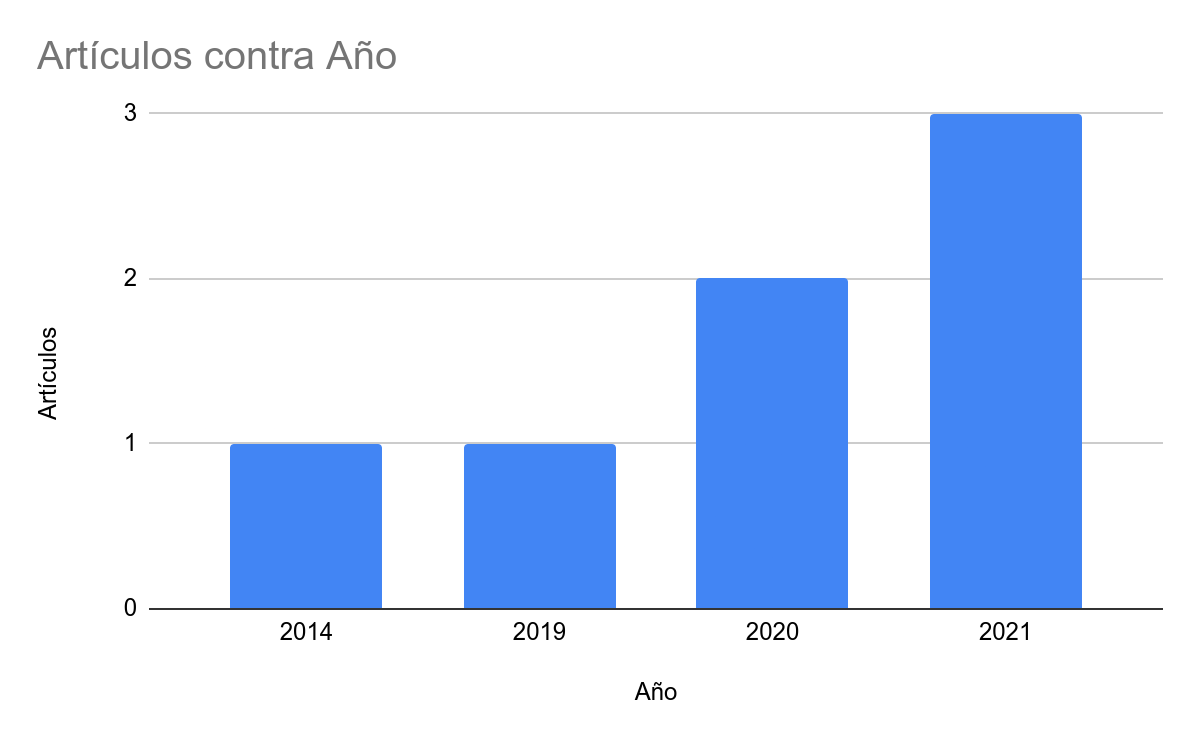
\includegraphics[width=0.8\textwidth]{img_03.png}
  \caption{N\'umero de art\'iculos por a\~no}
  \label{fig:articulos-por-anio}
\end{figure}

\section{Informaci\'on extra\'ida general}
\label{sec:info-extraida}

Toda la informaci\'on que se encontr\'o relevante en cada art\'iculo seleccionado fue extra\'ida y analizada para posteriormente ser incorporada como ayuda para la elaboraci\'on del proyecto de tesis (ver Tabla~\ref{tab:resumen-articulos}).

\begin{longtable}{|p{2.5cm}|p{2.5cm}|p{2.5cm}|p{2.5cm}|p{2.5cm}|}
\caption{Resumen de la informaci\'on extra\'ida por art\'iculo} \label{tab:resumen-articulos} \\
\hline
\textbf{Autor(es)} & \textbf{Indicadores SC} & \textbf{Indicadores Inst.} & \textbf{M\'etodo extracci\'on} & \textbf{Tecnolog\'ia} \\
\hline
\endfirsthead
\hline
\textbf{Autor(es)} & \textbf{Indicadores SC} & \textbf{Indicadores Inst.} & \textbf{M\'etodo extracci\'on} & \textbf{Tecnolog\'ia} \\
\hline
\endhead
\hline
\endfoot

\textcite{cutter2014} & Social Capital, Population Poverty & Emergency Services & Descarga manual de bases de datos p\'ublicas & SPSS \\
\hline
\textcite{villagra2017} & Civic Organizations, Population Poverty & Tsunami Drills & Descarga manual de bases de datos municipales y gubernamentales & R \\
\hline
\textcite{kamara2019} & Social networks, Community participation & Institutional support & Encuestas y entrevistas & SPSS \\
\hline
\textcite{heinzlef2020} & Social vulnerability & Emergency response & Bases de datos geoespaciales & GIS \\
\hline
\textcite{rumson2020} & Socioeconomic factors & Governance & Bases de datos ambientales & GIS, R \\
\hline
\textcite{moghadas2019} & Social capital & Institutional capacity & Encuestas & SPSS, AHP \\
\hline
\textcite{abrash2021} & Public health outcomes & Emergency preparedness & Revisi\'on sistem\'atica & -- \\
\hline
\textcite{muhamad2021} & Exposure elements & Disaster databases & Bases de datos locales & GIS \\
\hline
\textcite{wang2021} & Community engagement & Information dissemination & Twitter API & Python \\
\hline
\end{longtable}

\section{Principales hallazgos y factores claves}
\label{sec:hallazgos}

Uno de los hallazgos que llaman la atenci\'on a simple vista es que si bien para este estudio se contempla la dimensi\'on ``sociocomunitaria'', en todas las investigaciones analizadas estas aparecen separadas como ``Dimensi\'on social'' y ``Dimensi\'on comunitaria''.

Se realiz\'o un gr\'afico (ver Figura~\ref{fig:dimensiones-analizadas}) para apreciar de mejor manera la cantidad de dimensiones especificadas en cada investigaci\'on:

\begin{figure}[H]
  \centering
  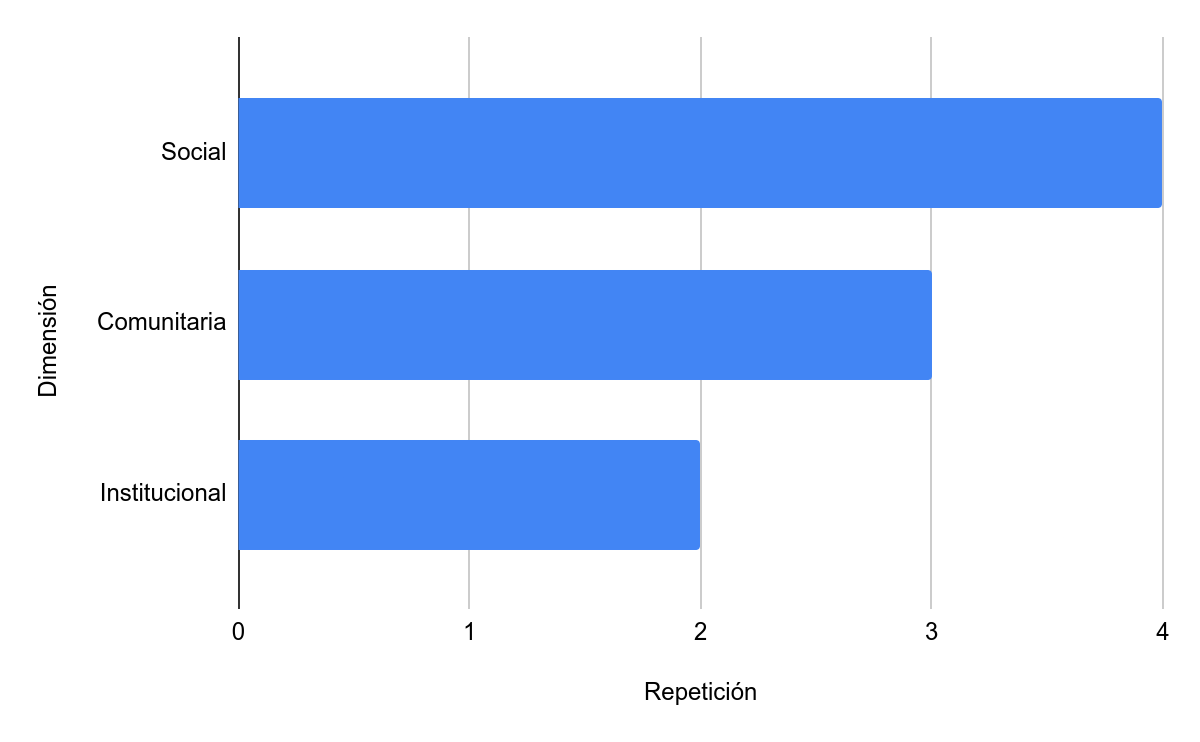
\includegraphics[width=0.8\textwidth]{img_04.png}
  \caption{Cantidad de veces que se analiz\'o cada dimensi\'on en las investigaciones}
  \label{fig:dimensiones-analizadas}
\end{figure}

De esta forma, se puede ver c\'omo la dimensi\'on social es la m\'as analizada con cuatro coincidencias en los \textit{papers}, mientras que la menos analizada es la dimensi\'on institucional, con dos coincidencias.

Tambi\'en se agreg\'o la diferencia en la cantidad de indicadores por cada dimensi\'on, como se aprecia en la Figura~\ref{fig:indicadores-por-dimension}:

\begin{figure}[H]
  \centering
  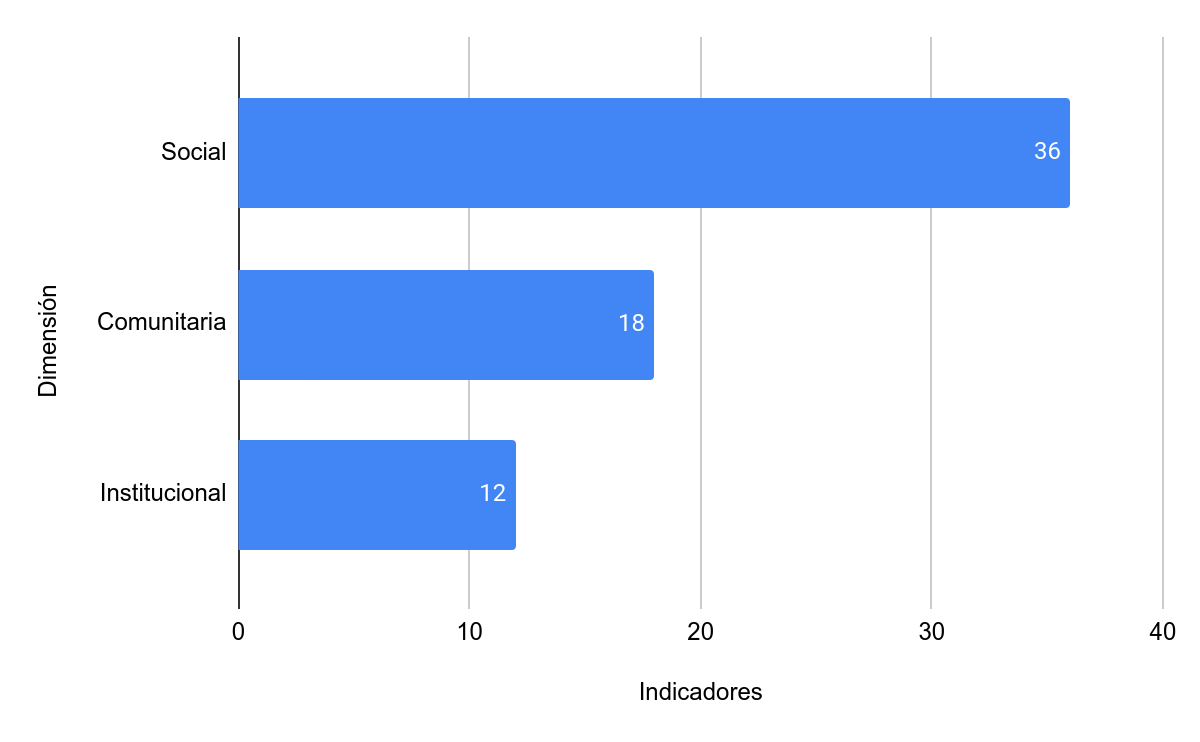
\includegraphics[width=0.8\textwidth]{img_05.png}
  \caption{Cantidad de indicadores totales por dimensi\'on}
  \label{fig:indicadores-por-dimension}
\end{figure}

En este caso se aprecia que las dimensiones social y f\'isica son las que agrupan m\'as indicadores en las investigaciones revisadas. Sin embargo, al calcular el promedio de indicadores por cada aparici\'on de dimensi\'on en los art\'iculos (ver Figura~\ref{fig:promedio-indicadores}), se observa que la dimensi\'on institucional, a pesar de ser la menos frecuente, presenta un promedio alto de indicadores cuando aparece.

\begin{figure}[H]
  \centering
  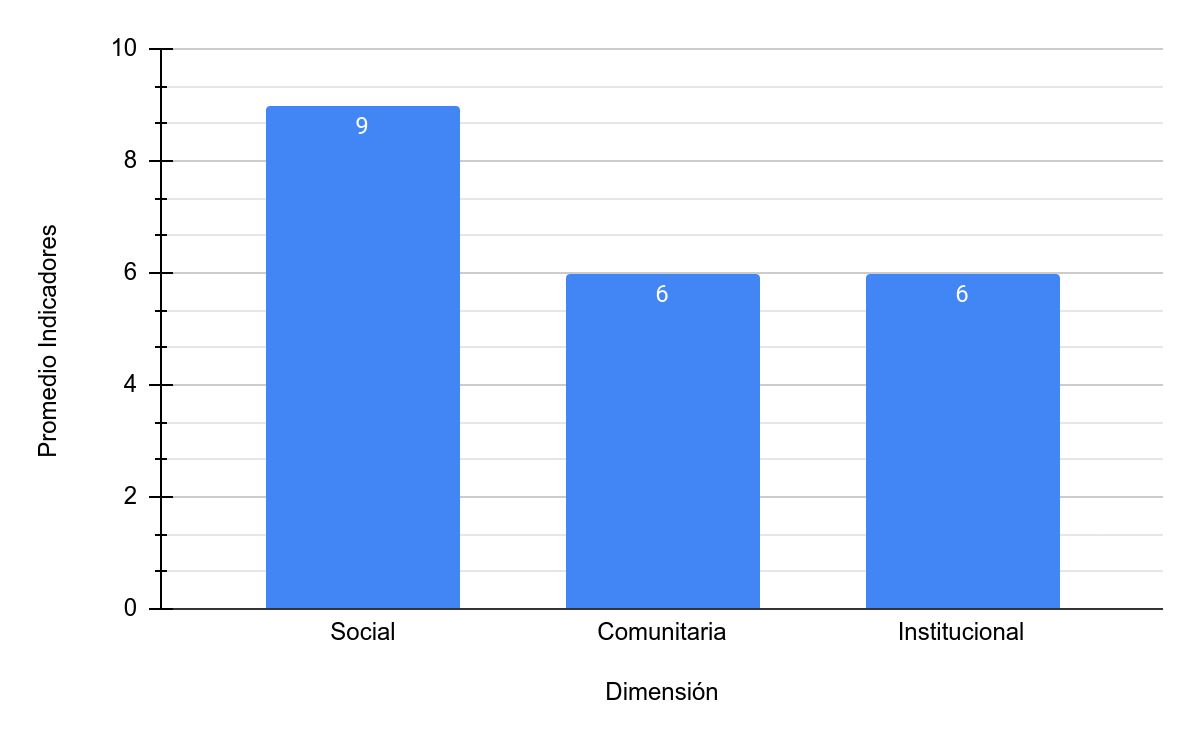
\includegraphics[width=0.8\textwidth]{img_06.png}
  \caption{Promedio de indicadores por aparici\'on de dimensi\'on en los art\'iculos}
  \label{fig:promedio-indicadores}
\end{figure}


% =============================================================================
% CAPITULO 3: VIABILIDAD DE INDICADORES
% =============================================================================
\chapter{VIABILIDAD DE INDICADORES}
\label{ch:viabilidad}

En este cap\'itulo se analiza la viabilidad de extracci\'on autom\'atica de cada indicador del modelo CORE en las dimensiones sociocomunitaria e institucional. Para cada indicador se identifican las fuentes de datos disponibles, el formato en que se encuentran, la segmentaci\'on geogr\'afica y las tareas necesarias para su incorporaci\'on al sistema.

Dentro del modelo CORE se especifican los indicadores correspondientes a las dimensiones sociocomunitaria e institucional que ser\'an objeto de an\'alisis (ver Anexo~\ref{app:indicadores-core}). La finalidad de esta b\'usqueda es analizar cu\'ales indicadores son viables para realizar la extracci\'on autom\'atica de sus datos.

\section{Population Poverty (PP)}
\label{sec:pp}

PP hace referencia a la tasa de pobreza de la poblaci\'on. El indicador puede expresarse como porcentaje directo o calcularse a partir de datos en bruto.

Los resultados de la investigaci\'on se pueden apreciar en la Tabla~\ref{tab:pp}:

\begin{table}[H]
\centering
\caption{Resumen de la investigaci\'on sobre Population Poverty}
\label{tab:pp}
\begin{tabular}{|p{3cm}|p{2.5cm}|p{2cm}|p{2cm}|p{3cm}|}
\hline
\textbf{Fuente} & \textbf{Tipo dato} & \textbf{Segm.} & \textbf{Formato} & \textbf{Notas} \\
\hline
BCN \parencite{bcn-a} & Porcentaje y datos en bruto & Comunal & Tabla HTML & Requiere \textit{web scraping} \\
\hline
Statista \parencite{statista} & Porcentaje & Nacional & Tabla & Requiere pago \\
\hline
DataSocial \parencite{datasocial} & Datos en bruto & Regional & .xls & Descarga directa \\
\hline
\end{tabular}
\end{table}

En este caso se observa que la informaci\'on de la BCN requiere t\'ecnicas de \textit{web scraping} para obtener los datos de las tablas HTML, mientras que la fuente de Statista fue descartada por requerir una suscripci\'on pagada. La fuente del Ministerio de Desarrollo Social ofrece la descarga directa en formato XLS.

\section{Social Capital -- Civic Participation (SCCP)}
\label{sec:sccp}

SCCP hace referencia al porcentaje de la poblaci\'on que participa activamente en procesos c\'ivicos (votaciones).

\begin{table}[H]
\centering
\caption{Resumen de la investigaci\'on sobre Civic Participation}
\label{tab:sccp}
\begin{tabular}{|p{3cm}|p{2.5cm}|p{2cm}|p{2cm}|p{3cm}|}
\hline
\textbf{Fuente} & \textbf{Tipo dato} & \textbf{Segm.} & \textbf{Formato} & \textbf{Notas} \\
\hline
SERVEL \parencite{servel} & Datos en bruto & Comunal & .csv & \'Unica fuente identificada \\
\hline
\end{tabular}
\end{table}

La informaci\'on es compleja de encontrar debido a que solo se identific\'o una fuente. El Servicio Electoral de Chile (SERVEL) provee datos en formato CSV que pueden ser descargados directamente.

\section{Social Capital -- Civic Organizations (SCCO)}
\label{sec:scco}

SCCO hace referencia a la raz\'on de organizaciones civiles por cada 1.000 habitantes por territorio.

\begin{table}[H]
\centering
\caption{Resumen de la investigaci\'on sobre Civic Organizations}
\label{tab:scco}
\begin{tabular}{|p{3cm}|p{2.5cm}|p{2cm}|p{2cm}|p{3cm}|}
\hline
\textbf{Fuente} & \textbf{Tipo dato} & \textbf{Segm.} & \textbf{Formato} & \textbf{Notas} \\
\hline
BCN \parencite{bcn-b} & Datos en bruto & Comunal & JSON, XLS, CSV, Tabla & M\'ultiples formatos disponibles \\
\hline
\end{tabular}
\end{table}

La BCN provee datos de organizaciones comunitarias en m\'ultiples formatos, incluyendo una API JSON que facilita la extracci\'on autom\'atica. Cada municipio posee sus propias fuentes de datos, pero la BCN centraliza esta informaci\'on a nivel comunal.

\section{Social Capital -- Emergency Organizations (SCEO)}
\label{sec:sceo}

SCEO hace referencia a la raz\'on de voluntarios en organizaciones de emergencia por cada 1.000 habitantes.

No se encontr\'o una fuente de datos p\'ublica centralizada para este indicador. La informaci\'on sobre voluntarios en organizaciones de emergencia depende de cada municipalidad y no se encuentra disponible de manera uniforme. Por esta raz\'on, este indicador no pudo ser implementado en el sistema.

\section{Tsunami Drills}
\label{sec:td}

Tsunami Drills hace referencia a la cantidad de simulacros de tsunami realizados en un per\'iodo de tiempo definido.

\begin{table}[H]
\centering
\caption{Resumen de la investigaci\'on sobre Tsunami Drills}
\label{tab:td}
\begin{tabular}{|p{3cm}|p{2.5cm}|p{2cm}|p{2cm}|p{3cm}|}
\hline
\textbf{Fuente} & \textbf{Tipo dato} & \textbf{Segm.} & \textbf{Formato} & \textbf{Notas} \\
\hline
ONEMI \parencite{onemi} & Datos en bruto & Nacional & Tabla HTML & Requiere \textit{web scraping} \\
\hline
MINEDUC \parencite{mineduc2022} & Datos en bruto & Nacional & Art\'iculo HTML & Requiere \textit{web scraping} \\
\hline
\end{tabular}
\end{table}

En este caso se observa que ninguno de los sitios que contienen informaci\'on sobre los simulacros de tsunami presenta los datos en un formato listo para ser trabajado. La \'unica forma de obtener esta informaci\'on es por medio de t\'ecnicas de \textit{web scraping}.

\section{Special Needs Population (SNP)}
\label{sec:snp}

SNP hace referencia al porcentaje de la poblaci\'on que padece alg\'un tipo de discapacidad.

\begin{table}[H]
\centering
\caption{Resumen de la investigaci\'on sobre Special Needs Population}
\label{tab:snp}
\begin{tabular}{|p{3cm}|p{2.5cm}|p{2cm}|p{2cm}|p{3cm}|}
\hline
\textbf{Fuente} & \textbf{Tipo dato} & \textbf{Segm.} & \textbf{Formato} & \textbf{Notas} \\
\hline
Obs. Social \parencite{observatoriosocial} & Porcentaje y datos en bruto & Comunal & .xls, .sav, .dta & Descarga directa \\
\hline
INE \parencite{ine-b} & Datos en bruto & Regional & .sav, .dat & Descarga directa \\
\hline
BCN \parencite{bcn-c} & Datos en bruto & Comunal & Tabla HTML & Requiere \textit{scraping} m\'inimo \\
\hline
\end{tabular}
\end{table}

La mayor\'ia de los datos se encuentra en un formato listo para ser utilizado y solo en un sitio web es necesario realizar t\'ecnicas de \textit{web scraping}.

\section{Conclusiones del an\'alisis de viabilidad}
\label{sec:conclusiones-viabilidad}

Las conclusiones obtenidas en este apartado investigativo son m\'ultiples:

En primer lugar se observa que muchos de estos datos requeridos se encuentran en un formato de f\'acil acceso y listos para ser descargados. En estos casos se puede dise\~nar el software para que tenga un fuerte \'enfasis en la descarga de informaci\'on omitiendo el \textit{scraping} y pasando directamente a ser transformada.

En segundo lugar, la mayor\'ia de los datos se presenta en formato de tabla, por lo que el software podr\'ia implementar un mecanismo de detecci\'on autom\'atica de tablas.

En tercer lugar, los datos que dependen de cada municipalidad requieren una b\'usqueda espec\'ifica por sitio web, lo que implica m\'odulos de extracci\'on personalizados.

En cuarto lugar, los formatos no est\'andar requieren m\'odulos espec\'ificos de \textit{scraping} adaptados a la estructura HTML de cada fuente.


% =============================================================================
% CAPITULO 4: HERRAMIENTAS DE DESARROLLO
% =============================================================================
\chapter{HERRAMIENTAS DE DESARROLLO}
\label{ch:herramientas}

Para la elecci\'on de las herramientas de desarrollo a utilizar se consideraron diversos par\'ametros, entre ellos:

\begin{itemize}
  \item Herramientas que se ajusten a las necesidades que busca resolver el equipo de investigadores.
  \item La popularidad y uso de las tecnolog\'ias. De esta manera se facilita la b\'usqueda de desarrolladores para mantener y escalar el software a largo plazo.
  \item Tecnolog\'ias con las cuales ya se posee cierta experiencia.
\end{itemize}

Con la finalidad de que el entorno de desarrollo sea reproducible por el equipo de investigaci\'on, en la Tabla~\ref{tab:stack} se declaran las versiones exactas con las que fue construido y validado el sistema. Las secciones siguientes justifican cada una de estas elecciones.

\begin{table}[H]
\centering
\caption{Stack tecnol\'ogico y versiones utilizadas}
\label{tab:stack}
\begin{tabular}{|p{4cm}|p{4.5cm}|p{3cm}|}
\hline
\textbf{Componente} & \textbf{Tecnolog\'ia} & \textbf{Versi\'on} \\
\hline
Lenguaje & TypeScript & 5.9.3 \\
\hline
Entorno de ejecuci\'on & Node.js & 22 LTS (\textit{jod}) \\
\hline
Base de datos & MongoDB & 6 \\
\hline
\textit{Framework} web & Express & 4.22.2 \\
\hline
{\itshape ODM} & Mongoose & 6.13.10 \\
\hline
\textit{Parsing} de HTML & Cheerio & 1.2.0 \\
\hline
Cliente HTTP & request-promise & 4.2.6 \\
\hline
Navegador automatizado & Puppeteer & 24.40.0 \\
\hline
Validaci\'on de esquemas & Zod & 4.3.6 \\
\hline
\textit{Logging} & Pino & 8.21.0 \\
\hline
Tareas programadas & node-cron & 4.2.1 \\
\hline
Pruebas & Jest & 29.7.0 \\
\hline
Contenedores & Docker Compose & \textit{Compose Specification} \\
\hline
Visualizaci\'on & Metabase & \texttt{latest} \\
\hline
Control de versiones & Git & --- \\
\hline
\end{tabular}
\end{table}

La versi\'on de Node.js se fija mediante el archivo \texttt{.nvmrc} con el alias \texttt{lts/jod}, que corresponde a la l\'inea 22 de soporte extendido. Esta decisi\'on responde a que las versiones recientes de Cheerio y de sus dependencias transitivas requieren caracter\'isticas de m\'odulos ECMAScript no disponibles en las l\'ineas anteriores. La \'unica versi\'on no fijada es la de Metabase, cuya imagen Docker se referencia mediante la etiqueta \texttt{latest}: al tratarse de una herramienta de visualizaci\'on externa al flujo ETL, su versi\'on exacta no compromete la reproducibilidad de los resultados del sistema.

\section{Lenguaje de programaci\'on}
\label{sec:lenguaje}

El lenguaje de programaci\'on elegido para el desarrollo del software es TypeScript. Un lenguaje que permite el desarrollo tanto en el \textit{frontend} como en el \textit{backend}.

TypeScript es un superconjunto de funcionalidades que extienden la sintaxis de Javascript, dot\'andolo de tipado est\'atico y de objetos basados en clases \parencite{typescript}. En resumen, permite aumentar la probabilidad de detectar errores en el c\'odigo, como tambi\'en hacer este m\'as legible.

La elecci\'on de este lenguaje es debido principalmente a la gran popularidad que posee Javascript, siendo en estos momentos uno de los lenguajes m\'as utilizados a nivel mundial, con un 68,62\% de preferencia seg\'un una encuesta realizada en el a\~no 2021 \parencite{stackoverflow2021}.

\section{Base de datos}
\label{sec:base-datos}

Se decidi\'o utilizar una base de datos no relacional. Espec\'ificamente la base de datos MongoDB \parencite{mongodb}.

La elecci\'on de esta base de datos es debido a la informaci\'on que se desea almacenar. Los datos deseados no poseen un esquema previamente definido, ya que cada indicador del modelo CORE posee una estructura distinta. Por lo que utilizar una base de datos relacional (como MySQL o PostgreSQL) aumentar\'ia la complejidad en caso de querer realizar cambios en una etapa avanzada del proyecto.

Adicionalmente, MongoDB permite almacenar documentos con estructuras heterog\'eneas dentro de una misma colecci\'on, lo cual facilita la persistencia de datos provenientes de fuentes diversas sin necesidad de migraciones complejas.

\section{Entorno de ejecuci\'on}
\label{sec:entorno}

El entorno de ejecuci\'on predilecto actualmente para el desarrollo de programas con Javascript/TypeScript es Node.js \parencite{nodejs}.

Node.js posee una madurez de m\'as de 15 a\~nos. Est\'a dise\~nado para crear aplicaciones escalables y orientado al uso de eventos as\'incronos.

Su simplicidad permite desarrollar aplicaciones en poco tiempo, posee un sistema de paquetes (npm) en constante crecimiento que permite a los desarrolladores implementar m\'ultiples herramientas y m\'odulos. Adem\'as, al poseer un n\'ucleo liviano, da una ventaja en el tama\~no final del software, ya que se utilizan solo las funcionalidades que se deseen implementar.

A continuaci\'on se muestra una lista de las librer\'ias principales y secundarias m\'as relevantes que se utilizan, junto con una peque\~na descripci\'on.

\subsection{Librer\'ias principales}
\label{sec:librerias-principales}

\begin{itemize}
  \item \textbf{cheerio} \parencite{cheerio}: Permite analizar la estructura de las p\'aginas web permitiendo la extracci\'on y manipulaci\'on de los datos. Se utiliza para el \textit{parsing} de HTML en los m\'odulos que requieren \textit{web scraping}.
  \item \textbf{express} \parencite{express}: Es actualmente el \textit{framework} m\'as popular de Node.js. Permite el manejo de peticiones HTTP y desarrollo de APIs.
  \item \textbf{mongoose} \parencite{mongoose}: Es un ODM que permite escribir consultas y crear esquemas para la base de datos MongoDB. Se utiliza para definir los modelos de datos de cada indicador y gestionar el almacenamiento.
  \item \textbf{request-promise}: Permite hacer llamadas HTTP. Se utiliza para obtener el HTML de una p\'agina web o realizar peticiones a APIs externas.\footnote{El desarrollo inicial del prototipo utilizaba la librer\'ia \textit{request}, de interfaz basada en \textit{callbacks}. Se migr\'o a \textit{request-promise}, que envuelve la misma implementaci\'on exponiendo promesas, con el fin de integrarla con la sintaxis \texttt{async/await} que emplea el flujo ETL. Ambas librer\'ias fueron declaradas \textit{deprecated} por sus autores en febrero de 2020 \parencite{requestpromise}; su reemplazo se aborda en la secci\'on~\ref{sec:trabajo-futuro} como deuda t\'ecnica.}
  \item \textbf{puppeteer} \parencite{puppeteer}: Permite la automatizaci\'on de un navegador web. Se utiliza para extraer informaci\'on de p\'aginas que renderizan su contenido mediante Javascript, donde \textit{cheerio} no es suficiente.
  \item \textbf{zod} \parencite{zod}: Librer\'ia de validaci\'on y declaraci\'on de esquemas. Se utiliza para validar la configuraci\'on de los indicadores en tiempo de construcci\'on, asegurando que cada indicador posea los campos requeridos antes de ser registrado en el sistema.
  \item \textbf{pino} \parencite{pino}: Librer\'ia de \textit{logging} de alto rendimiento. Se utiliza como \textit{logger} centralizado del sistema, generando registros tanto en consola (durante el desarrollo) como en archivos de log para auditor\'ia.
  \item \textbf{node-cron} \parencite{nodecron}: Permite la programaci\'on de tareas peri\'odicas mediante expresiones cron. Se utiliza para automatizar la ejecuci\'on de los procesos de extracci\'on seg\'un la frecuencia definida para cada indicador.
\end{itemize}

\subsection{Librer\'ias secundarias}
\label{sec:librerias-secundarias}

\begin{itemize}
  \item \textbf{eslint}: Es una herramienta que permite ayudar en la detecci\'on de errores de c\'odigo y mantener este m\'as legible.
  \item \textbf{prettier}: Es una herramienta de formateo de c\'odigo que asegura un estilo consistente en todo el proyecto.
  \item \textbf{nodemon}: Es una herramienta que permite actualizar autom\'aticamente la ejecuci\'on de la aplicaci\'on en cuanto detecta cambios en el desarrollo.
  \item \textbf{typescript}: Permite escribir c\'odigo de TypeScript y transpilarlo a c\'odigo de Javascript.
  \item \textbf{jest} \parencite{jest}: \textit{Framework} que permite realizar pruebas unitarias y de integraci\'on.
\end{itemize}

\section{Contenedores}
\label{sec:contenedores}

Para facilitar el despliegue y la reproducibilidad del entorno de desarrollo, se utiliza Docker junto con Docker Compose \parencite{docker}.

Docker permite crear contenedores aislados que encapsulan la aplicaci\'on y sus dependencias, mientras que Docker Compose permite definir y orquestar m\'ultiples servicios de forma declarativa. En el caso de este proyecto, se definen tres servicios: la base de datos MongoDB, una interfaz de administraci\'on (Mongo Express) y una herramienta de visualizaci\'on de datos (Metabase).

Esta decisi\'on permite que cualquier integrante del equipo de investigaci\'on pueda levantar el entorno completo con un solo comando, sin necesidad de instalar ni configurar cada servicio de forma manual.

\section{Visualizaci\'on de datos}
\label{sec:visualizacion}

Para la visualizaci\'on de los datos almacenados se utiliza Metabase \parencite{metabase}, una herramienta de \textit{Business Intelligence} de c\'odigo abierto que permite crear \textit{dashboards} y consultas sobre bases de datos sin necesidad de escribir c\'odigo.

Metabase se conecta directamente a MongoDB y permite a los investigadores visualizar los indicadores extra\'idos por medio de gr\'aficos, tablas y filtros. Los \textit{dashboards} se actualizan autom\'aticamente cada vez que se consultan, reflejando los datos m\'as recientes almacenados en la base de datos.

La elecci\'on de Metabase por sobre un \textit{frontend} personalizado (como Angular o React) se debe a que el objetivo principal del proyecto es la extracci\'on y el procesamiento de datos, no la construcci\'on de una interfaz gr\'afica. Metabase permite cumplir con el objetivo de poner a disposici\'on los datos mediante anal\'iticas sin requerir desarrollo adicional.

\section{Sistema de control de versiones}
\label{sec:control-versiones}

Un sistema de control de versiones permite rastrear y gestionar los cambios que son realizados dentro de un c\'odigo de software. Estas herramientas ayudan a los equipos de desarrollo a gestionar los cambios en el c\'odigo fuente \parencite{atlassian}.

En este caso, se opt\'o por utilizar Git \parencite{git}. Un sistema de control de versiones creado por Linus Torvalds, el cual est\'a centrado en ser eficiente, confiable y mantenible. Actualmente es utilizado por m\'as de un 93\% de los desarrolladores \parencite{stackoverflow2021}, convirti\'endose en una de las tecnolog\'ias indispensables para el desarrollo de software.


% =============================================================================
% CAPITULO 5: DISENO DE PROTOTIPO
% =============================================================================
\chapter{DISE\~NO DE PROTOTIPO}
\label{ch:prototipo}

Antes de comprometerse con una arquitectura definitiva, se construy\'o un prototipo cuyo prop\'osito no era producir software de producci\'on sino responder emp\'iricamente una pregunta de dise\~no: ?`qu\'e parte del proceso ETL var\'ia entre una fuente de datos y otra, y qu\'e parte permanece constante? La respuesta a esa pregunta determina qu\'e debe ser fijo en el n\'ucleo del sistema y qu\'e debe ser intercambiable.

Este cap\'itulo describe el prototipo construido, los artefactos que produjo y las limitaciones que revel\'o. Las decisiones arquitect\'onicas que se derivan de estas limitaciones se detallan en el Cap\'itulo~\ref{ch:desarrollo}.

\section{Alcance del prototipo}
\label{sec:alcance-prototipo}

El prototipo se acot\'o deliberadamente a dos indicadores de la dimensi\'on sociocomunitaria (tasa de pobreza y poblaci\'on carente de servicios b\'asicos) extra\'idos desde una \'unica fuente. Esta restricci\'on fue intencional: con dos indicadores distintos sobre una misma fuente es posible observar qu\'e c\'odigo se repite entre ambos y cu\'al es espec\'ifico de cada uno, que es precisamente la informaci\'on que se buscaba. El indicador de poblaci\'on carente de servicios b\'asicos no forma parte de los analizados en el Cap\'itulo~\ref{ch:viabilidad}; se incluy\'o porque comparte fuente y formato de presentaci\'on con la tasa de pobreza, lo que permit\'ia comparar dos extracciones sobre un mismo portal.

El prototipo cubri\'o las tres etapas del proceso ETL de extremo a extremo: obtenci\'on del HTML, extracci\'on de los valores y persistencia en MongoDB. No se implementaron en esta etapa la programaci\'on de tareas peri\'odicas, el manejo de errores tipados ni la exposici\'on mediante una API, por no ser necesarios para responder la pregunta de dise\~no planteada.

\section{Fuentes de datos exploradas}
\label{sec:fuentes-exploradas}

Se realiz\'o una b\'usqueda manual en internet para encontrar p\'aginas web que dispusieran de informaci\'on pertinente a los indicadores. Si bien se encontraron diversas fuentes, la mayor\'ia ya se encontraba en formatos descargables. En la Figura~\ref{fig:proto-pobreza} y Figura~\ref{fig:proto-servicios} se muestran ejemplos de la informaci\'on sociocomunitaria encontrada.

La observaci\'on relevante de esta exploraci\'on es que ambos indicadores, pese a provenir del mismo portal y presentarse con el mismo formato visual, no compart\'ian estructura HTML: difer\'ian en la cantidad de columnas, en el orden de las filas y en la forma de expresar los valores. Es decir, la variabilidad entre fuentes no depende del proveedor de los datos sino de cada p\'agina en particular.

\begin{figure}[H]
  \centering
  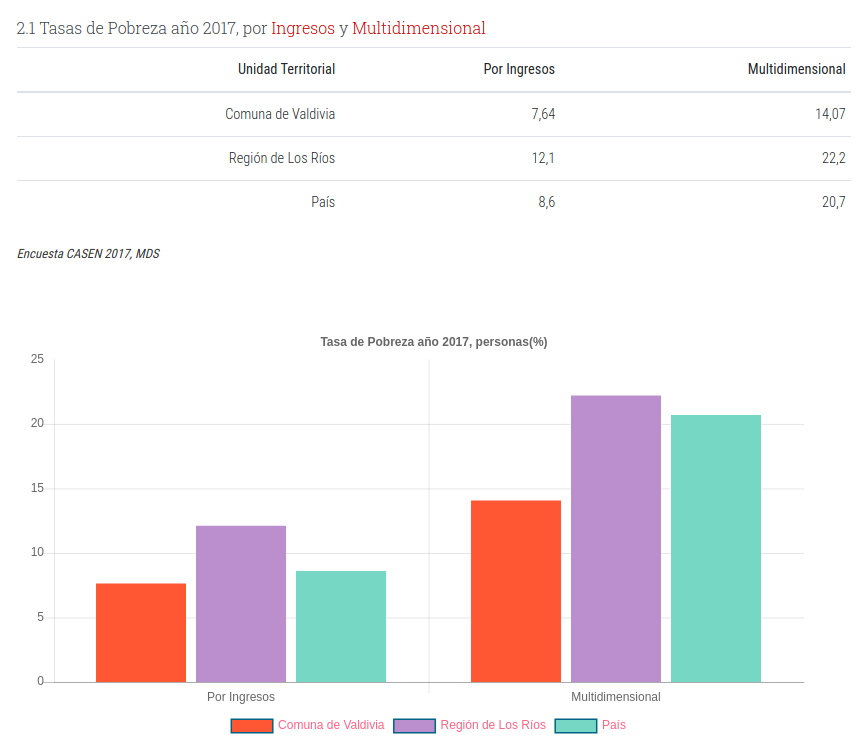
\includegraphics[width=0.8\textwidth]{img_08.png}
  \caption[Informaci\'on sociocomunitaria sobre tasa de pobreza en el a\~no 2017]{Informaci\'on sociocomunitaria sobre tasa de pobreza en el a\~no 2017. Fuente: \textcite{bcn-a}}
  \label{fig:proto-pobreza}
\end{figure}

\begin{figure}[H]
  \centering
  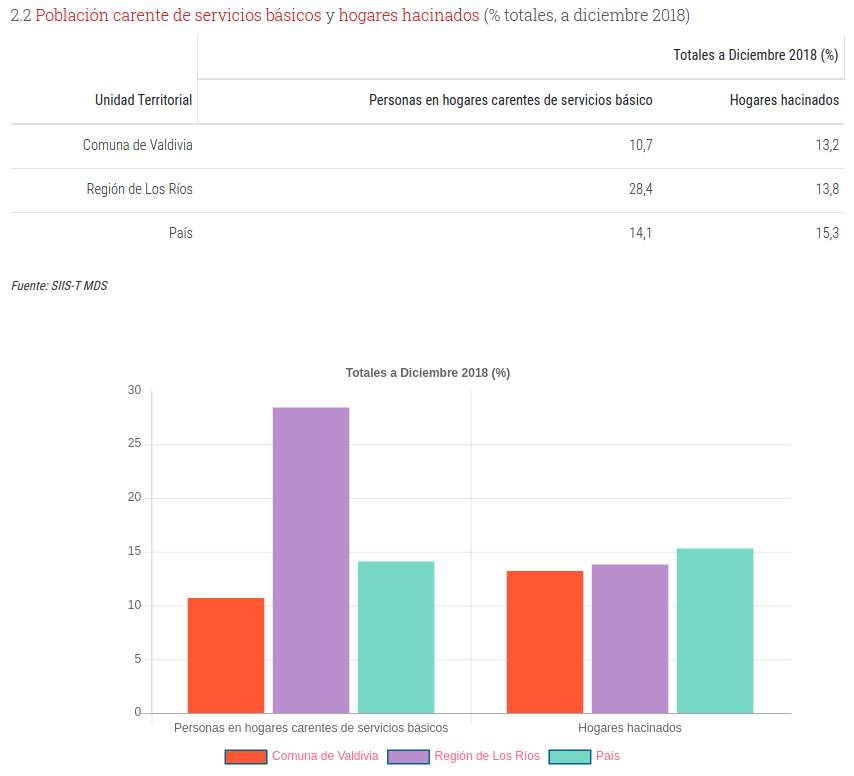
\includegraphics[width=0.8\textwidth]{img_09.png}
  \caption[Informaci\'on sociocomunitaria sobre poblaci\'on carente de servicios b\'asicos y hogares hacinados en el a\~no 2018]{Informaci\'on sociocomunitaria sobre poblaci\'on carente de servicios b\'asicos y hogares hacinados en el a\~no 2018. Fuente: \textcite{bcn-a}}
  \label{fig:proto-servicios}
\end{figure}

\section{Modelo de datos inicial}
\label{sec:modelo-datos-inicial}

Para el modelo de la base de datos, se comenz\'o con la idea de almacenar la informaci\'on de la p\'agina web como tal (URL de origen y fecha de extracci\'on), para luego ir desglosando la informaci\'on en modelos m\'as espec\'ificos. En la Figura~\ref{fig:proto-interface-web} se presenta la \textit{interface} inicial.

\begin{figure}[H]
  \centering
  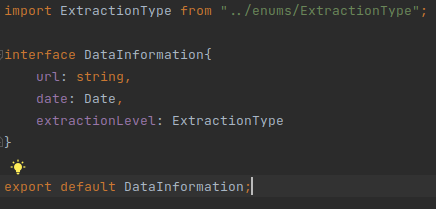
\includegraphics[width=0.6\textwidth]{img_10.png}
  \caption{\textit{Interface} para la informaci\'on de la p\'agina web}
  \label{fig:proto-interface-web}
\end{figure}

Una vez obtenida la informaci\'on base, se continu\'o con los modelos para cada indicador (ver Figuras~\ref{fig:proto-interface-pobreza} y~\ref{fig:proto-interface-servicios}). Cada indicador requiri\'o su propia \textit{interface}, ya que los campos de la tasa de pobreza no coinciden con los de la poblaci\'on carente de servicios b\'asicos. Esta constataci\'on, que el esquema de datos es propio de cada indicador y no puede unificarse, fue el argumento decisivo para optar por una base de datos documental por sobre una relacional, seg\'un se justific\'o en la secci\'on~\ref{sec:base-datos}.

\begin{figure}[H]
  \centering
  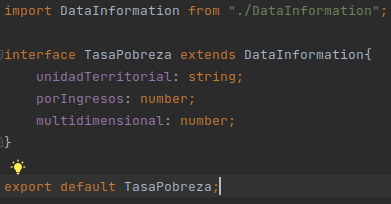
\includegraphics[width=0.6\textwidth]{img_11.png}
  \caption{\textit{Interface} para tasa de pobreza}
  \label{fig:proto-interface-pobreza}
\end{figure}

\begin{figure}[H]
  \centering
  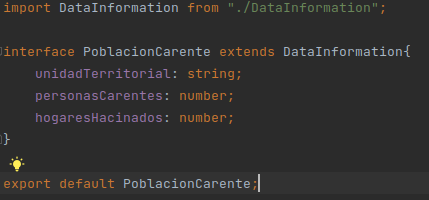
\includegraphics[width=0.6\textwidth]{img_12.png}
  \caption{\textit{Interface} para poblaci\'on carente de servicios b\'asicos y hogares hacinados}
  \label{fig:proto-interface-servicios}
\end{figure}

\section{Clases de extracci\'on}
\label{sec:clases-extraccion-prototipo}

Para la extracci\'on, se crearon tres clases (ver Figura~\ref{fig:proto-clases}) encargadas de las distintas etapas del proceso.

\begin{figure}[H]
  \centering
  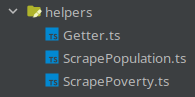
\includegraphics[width=0.5\textwidth]{img_13.png}
  \caption{Lista de clases utilizadas para la extracci\'on de la informaci\'on}
  \label{fig:proto-clases}
\end{figure}

La organizaci\'on de estas clases es en s\'i misma el hallazgo m\'as importante del prototipo. La clase \texttt{Getter} concentra la obtenci\'on del contenido de una URL y es reutilizable entre indicadores. En cambio, \texttt{ScrapePoverty} y \texttt{ScrapePopulation} son una clase completa por cada indicador, y dentro de cada una conviven la extracci\'on de los valores desde el HTML, su transformaci\'on al tipo de dato esperado y su persistencia en la base de datos.

Esta estructura presenta dos problemas que impiden escalarla a los 21 indicadores del modelo CORE. El primero es que agregar un indicador obliga a escribir una clase nueva que reimplementa las tres etapas desde cero, aunque dos de ellas sean casi id\'enticas a las ya existentes. El segundo es que, al estar las tres etapas mezcladas en un mismo m\'etodo, no es posible probar la extracci\'on de forma aislada ni sustituir una etapa sin reescribir las otras: un cambio en la estructura HTML de la fuente obliga a intervenir el mismo c\'odigo que realiza el guardado.

\section{Aprendizajes y transici\'on a la arquitectura final}
\label{sec:aprendizajes-prototipo}

El prototipo permiti\'o distinguir con evidencia qu\'e var\'ia entre indicadores y qu\'e permanece constante. Lo que var\'ia es la forma de acceder a la fuente, la manera de localizar los datos dentro del contenido obtenido, la transformaci\'on al tipo esperado y el criterio que identifica un registro como \'unico. Lo que permanece constante es el orden en que estas etapas se ejecutan.

Esta distinci\'on es la que define la arquitectura del sistema final: la secuencia de etapas pertenece al n\'ucleo y se escribe una sola vez, mientras que el contenido de cada etapa se declara por indicador. La Tabla~\ref{tab:prototipo-arquitectura} resume c\'omo cada limitaci\'on observada en el prototipo se traduce en un mecanismo concreto de la arquitectura final.

\begin{table}[H]
\centering
\caption{Limitaciones del prototipo y su resoluci\'on en la arquitectura final}
\label{tab:prototipo-arquitectura}
\begin{tabular}{|p{6cm}|p{6cm}|}
\hline
\textbf{Limitaci\'on observada en el prototipo} & \textbf{Mecanismo en la arquitectura final} \\
\hline
El acceso a la fuente var\'ia (HTML est\'atico, JSON, archivo descargable) y estaba resuelto solo para HTML & \textit{FetchAdapter} con implementaciones concretas por tipo de conexi\'on (secci\'on~\ref{sec:tipos-conexion}) \\
\hline
Localizar los datos exige c\'odigo distinto por cada p\'agina, incluso dentro de un mismo portal & \textit{ParseAdapter} declarado por indicador (secci\'on~\ref{sec:patron-adapter}) \\
\hline
Los valores se obtienen como texto gen\'erico y deben convertirse al tipo esperado & \textit{MapperAdapter} (secci\'on~\ref{sec:patron-adapter}) \\
\hline
La ejecuci\'on peri\'odica reinsertar\'ia registros ya existentes & \textit{HashAdapter} y restricci\'on de unicidad en el esquema (secci\'on~\ref{sec:duplicados}) \\
\hline
Las tres etapas conviven en una clase por indicador, impidiendo probarlas o sustituirlas por separado & \textit{ScrapeBase} orquesta la secuencia; cada m\'odulo solo aporta sus \textit{adapters} (secci\'on~\ref{sec:scrape-base}) \\
\hline
\end{tabular}
\end{table}

En s\'intesis, el prototipo no se descart\'o ni se traslad\'o tal cual: su estructura de tres etapas se conserv\'o como el flujo del sistema, pero se invirti\'o la relaci\'on entre lo gen\'erico y lo espec\'ifico. Donde el prototipo ten\'ia una clase por indicador que implementaba las tres etapas, la arquitectura final tiene una implementaci\'on \'unica de las tres etapas que recibe, por indicador, la porci\'on que efectivamente cambia.


% =============================================================================
% CAPITULO 6: DESARROLLO E IMPLEMENTACION
% =============================================================================
\chapter{DESARROLLO E IMPLEMENTACI\'ON}
\label{ch:desarrollo}

En este cap\'itulo se describe la arquitectura del software desarrollado, los patrones de dise\~no utilizados y la implementaci\'on de los m\'odulos de extracci\'on de datos. La arquitectura fue dise\~nada con el objetivo de que agregar un nuevo indicador al sistema requiera el m\'inimo esfuerzo posible, manteniendo la separaci\'on de responsabilidades y la reutilizaci\'on de componentes.

\section{Arquitectura general}
\label{sec:arquitectura}

El sistema se estructura en tres capas principales: el \textit{core}, los m\'odulos y la API, tal como se muestra en la Figura~\ref{fig:arquitectura-general}. El \textit{core} contiene las clases base, los \textit{adapters} abstractos y la l\'ogica de orquestaci\'on del flujo ETL. Los m\'odulos son implementaciones concretas para cada fuente de datos. La API expone los indicadores al exterior mediante \textit{endpoints} HTTP.

\begin{figure}[H]
  \centering
  \begin{tikzpicture}[
    font=\scriptsize,
    caja/.style={draw, rounded corners=2pt, align=center, minimum height=6mm,
                 inner xsep=2pt},
    capa/.style={draw, dashed, rounded corners=3pt, inner sep=4pt},
    flecha/.style={-{Stealth[length=1.8mm]}},
    externo/.style={caja, fill=black!8}
  ]

  % --- Capa API ---
  \node[caja, minimum width=26mm] (rutas)  at (2.0,0)    {Rutas HTTP};
  \node[caja, minimum width=26mm] (errh)   at (5.2,0)    {Manejador de errores};
  \node[capa, fit=(rutas)(errh),
        label={[font=\scriptsize\bfseries, xshift=-1mm]left:API}] (capaapi) {};

  % --- Capa Core ---
  \node[caja, minimum width=24mm] (factory) at (1.55,-2.05) {ScraperFactory};
  \node[caja, minimum width=20mm] (base)    at (4.15,-2.05) {ScrapeBase};
  \node[caja, minimum width=24mm] (builder) at (6.65,-2.05) {IndicatorBuilder};
  \node[caja, minimum width=22mm] (cron)    at (9.15,-2.05) {CronRegistry};
  \node[caja, minimum width=94mm] (adapters) at (5.35,-3.05)
       {\textit{Adapters} abstractos:
        Fetch $\cdot$ Parse $\cdot$ Mapper $\cdot$ Hash $\cdot$ Storage $\cdot$ Calculator};
  \node[capa, fit=(factory)(cron)(adapters),
        label={[font=\scriptsize\bfseries, xshift=-1mm]left:Core}] (capacore) {};

  % --- Capa Modulos ---
  \node[caja, minimum width=42mm] (med)  at (2.35,-5.1) {emergencias-desastres};
  \node[caja, minimum width=48mm] (mbcn) at (7.35,-5.1)
       {biblioteca-congreso-nacional};
  \node[capa, fit=(med)(mbcn),
        label={[font=\scriptsize\bfseries, xshift=-1mm]left:M\'odulos}] (capamod) {};

  % --- Elementos externos ---
  \node[externo, minimum width=24mm] (mongo) at (5.35,-6.75) {MongoDB};
  \node[externo, align=center] (fuentes) at (5.35,1.75)
       {Fuentes web\\MINEDUC $\cdot$ BCN};

  % --- Relaciones verticales ---
  \draw[flecha] (capaapi.south) -- node[right=1pt] {solicita indicador}
        (capacore.north);
  \draw[flecha] (capacore.south) -- node[right=1pt] {ejecuta flujo ETL}
        (capamod.north);
  \draw[flecha] (capamod.south) -- node[right=1pt] {persiste} (mongo.north);

  % --- Los modulos consultan las fuentes, no la API ---
  \draw[flecha] (capamod.east) -| node[below right=0pt and 1pt, pos=0.25]
        {consulta} (11.9,-5.1) -- (11.9,1.75) -- (fuentes.east);
  \end{tikzpicture}
  \caption{Arquitectura general del sistema: las tres capas y su relaci\'on con las fuentes externas y la base de datos}
  \label{fig:arquitectura-general}
\end{figure}

La comunicaci\'on entre las capas sigue un flujo unidireccional: la API recibe la solicitud, el \textit{ScraperFactory} obtiene el m\'odulo correspondiente, y el m\'odulo ejecuta el flujo ETL utilizando los \textit{adapters} configurados para ese indicador.

\section{Patrones de dise\~no}
\label{sec:patrones}

Se utilizaron diversos patrones de dise\~no para lograr una arquitectura extensible y con bajo acoplamiento. A continuaci\'on se describen los m\'as relevantes.

\subsection{Patr\'on Builder}
\label{sec:patron-builder}

El \textit{IndicatorBuilder} permite configurar cada indicador de forma declarativa, encadenando los m\'etodos de configuraci\'on y validando los datos con la librer\'ia Zod al momento de construir el indicador. Esto asegura que un indicador no pueda ser registrado en el sistema si le falta informaci\'on obligatoria como el nombre o la URL de la fuente. La Figura~\ref{fig:indicator-builder} muestra la configuraci\'on completa de uno de los indicadores implementados.

\begin{figure}[H]
\begin{lstlisting}[style=codigo, language=TypeScript]
"simulacros-2021": new IndicatorBuilder()
  .setName("Simulacros 2021")
  .setUrl("https://web.archive.org/web/20211026024955/https://" +
          "emergenciaydesastres.mineduc.cl/simulacros-2021/")
  .setFrequency(FREQUENCIES.once)
  .setFetchAdapter(new RequestPromiseAdapter())
  .setParseAdapter(new DateParserAdapter())
  .setMapperAdapter(new EmergenciaDesastresMapper())
  .setHashAdapter(new EmergenciaDesastresHashAdapter())
  .setStorageAdapter(new EmergenciasDesastresStorageAdapter())
  .setCalculatorAdapter(new TsunamiDrillsCalculatorAdapter())
  .build()
\end{lstlisting}
\caption{Configuraci\'on del indicador \texttt{simulacros-2021} mediante el \textit{IndicatorBuilder}}
\label{fig:indicator-builder}
\end{figure}

El indicador queda descrito por completo en esta declaraci\'on: no existe c\'odigo procedural asociado a \texttt{simulacros-2021} fuera de los \textit{adapters} que aqu\'i se le asignan. Agregar un indicador nuevo consiste en escribir un bloque equivalente y, cuando la fuente lo exige, implementar los \textit{adapters} que difieran de los ya disponibles. La llamada final a \texttt{build()} valida la configuraci\'on con Zod, de modo que un indicador incompleto falla al iniciar la aplicaci\'on y no en el momento de ejecutar la extracci\'on.

\subsection{Patr\'on Adapter}
\label{sec:patron-adapter}

Cada etapa del flujo ETL se define mediante un \textit{adapter} abstracto que establece la interfaz que deben implementar las clases concretas. Esto permite que un m\'odulo utilice un \textit{adapter} distinto para cada etapa sin modificar la l\'ogica central del sistema. Los \textit{adapters} definidos son:

\begin{itemize}
  \item \textbf{FetchAdapter}: Define c\'omo se obtienen los datos de la fuente (HTML, JSON, archivo).
  \item \textbf{ParseAdapter}: Define c\'omo se extrae la informaci\'on estructurada de los datos crudos.
  \item \textbf{MapperAdapter}: Define c\'omo se transforman los datos extra\'idos al formato que se almacena en la base de datos.
  \item \textbf{HashAdapter}: Genera una clave \'unica por registro para evitar duplicados.
  \item \textbf{StorageAdapter}: Controla el almacenamiento de los datos procesados.
  \item \textbf{CalculatorAdapter} (opcional): Calcula un resultado agregado a partir de los datos almacenados y lo persiste en una colecci\'on separada.
\end{itemize}

La Figura~\ref{fig:diagrama-adapters} presenta estos \textit{adapters} con sus m\'etodos abstractos, junto con las implementaciones concretas disponibles para la etapa de obtenci\'on de datos.

\begin{figure}[H]
  \centering
  \begin{tikzpicture}[
    font=\scriptsize,
    clase/.style={draw, rectangle split, rectangle split parts=2,
                  rectangle split part align=left, align=left,
                  text width=34mm, inner sep=3pt},
    abstracta/.style={clase, fill=black!5},
    herencia/.style={-{Triangle[open, length=2.5mm, width=2.5mm]}},
    nota/.style={font=\scriptsize\itshape}
  ]

  % --- Fila 1: adapters abstractos ---
  \node[abstracta] (fetch) {
    \textbf{\textlangle\textlangle abstract\textrangle\textrangle}\\\textbf{FetchAdapter}
    \nodepart{two}\texttt{fetch(url): Promise}};
  \node[abstracta, right=5mm of fetch] (parse) {
    \textbf{\textlangle\textlangle abstract\textrangle\textrangle}\\\textbf{ParseAdapter}
    \nodepart{two}\texttt{extract(raw): T[]}};
  \node[abstracta, right=5mm of parse] (mapper) {
    \textbf{\textlangle\textlangle abstract\textrangle\textrangle}\\\textbf{MapperAdapter}
    \nodepart{two}\texttt{map(input): Output}};

  % --- Fila 2 ---
  \node[abstracta, below=7mm of fetch] (hash) {
    \textbf{\textlangle\textlangle abstract\textrangle\textrangle}\\\textbf{HashAdapter}
    \nodepart{two}\texttt{generate(data): string}};
  \node[abstracta, below=7mm of parse] (storage) {
    \textbf{\textlangle\textlangle abstract\textrangle\textrangle}\\\textbf{StorageAdapter}
    \nodepart{two}\texttt{save(data): Promise}\\\texttt{find(): Promise}};
  \node[abstracta, below=7mm of mapper] (calc) {
    \textbf{\textlangle\textlangle abstract\textrangle\textrangle}\\\textbf{CalculatorAdapter}
    \nodepart{two}\texttt{calculate(data): R}\\\texttt{save(r, ind, mod)}\\\texttt{find(ind, mod)}};

  % --- Implementaciones concretas del FetchAdapter ---
  \node[clase, below=12mm of hash.south west, anchor=north west,
        text width=76mm] (concretos) {
    \textbf{Implementaciones concretas de FetchAdapter}
    \nodepart{two}
    \texttt{RequestPromiseAdapter}: HTML est\'atico\\
    \texttt{JsonFetchAdapter}: API JSON\\
    \texttt{PuppeteerAdapter}: p\'aginas renderizadas con Javascript\\
    \texttt{DownloadAdapter}: descarga de archivos CSV y XLSX};

  % Se rutea por la izquierda para no atravesar la caja de HashAdapter.
  \draw[herencia] (concretos.west) -- ++(-4mm,0) |- (fetch.west);

  \node[nota, right=5mm of concretos, text width=32mm, align=left] {
    Cada indicador declara\\
    una implementaci\'on\\
    por cada \textit{adapter};\\
    el \textit{Calculator} es\\
    el \'unico opcional.};
  \end{tikzpicture}
  \caption{Diagrama de clases de los \textit{adapters} con sus m\'etodos abstractos}
  \label{fig:diagrama-adapters}
\end{figure}

\subsection{Patr\'on Factory y Singleton}
\label{sec:patron-factory}

El \textit{ScraperFactory} es una clase \textit{Singleton} que funciona como registro central de m\'odulos. Cada m\'odulo se registra en el \textit{factory} al iniciar la aplicaci\'on, y puede ser obtenido por nombre para ejecutar la extracci\'on de un indicador espec\'ifico. Esto desacopla la l\'ogica de registro de la l\'ogica de ejecuci\'on.

De manera similar, el \textit{CronRegistry} es un \textit{Singleton} que registra tareas programadas para cada indicador seg\'un su frecuencia configurada, permitiendo la ejecuci\'on autom\'atica y peri\'odica del proceso de extracci\'on.

\subsection{Clase abstracta ScrapeBase}
\label{sec:scrape-base}

Todos los m\'odulos extienden la clase abstracta \textit{ScrapeBase}, la cual implementa el flujo ETL completo. El m\'etodo \texttt{init} orquesta las etapas en el siguiente orden:

\begin{enumerate}
  \item Se construye la URL reemplazando los par\'ametros din\'amicos (como el a\~no).
  \item El \textit{FetchAdapter} obtiene los datos crudos de la fuente.
  \item El \textit{ParseAdapter} extrae la informaci\'on estructurada.
  \item El \textit{MapperAdapter} normaliza la estructura de los datos.
  \item El \textit{HashAdapter} genera la clave \'unica de cada registro.
  \item El \textit{StorageAdapter} almacena los datos en MongoDB, ignorando duplicados.
  \item Si existe un \textit{CalculatorAdapter}, se calcula el resultado agregado y se almacena en la colecci\'on \texttt{indicator-results}, solo si el resultado difiere del \'ultimo almacenado.
\end{enumerate}

La Figura~\ref{fig:diagrama-secuencia} representa esta secuencia y las decisiones que la condicionan: la interrupci\'on del flujo cuando la extracci\'on no devuelve registros, el descarte de duplicados en el almacenamiento y la escritura condicional del resultado calculado.

\begin{figure}[H]
  \centering
  \begin{tikzpicture}[
    font=\scriptsize,
    actor/.style={draw, fill=black!5, minimum height=6mm, inner xsep=3pt,
                  align=center},
    linea/.style={dashed, gray},
    msj/.style={-{Stealth[length=1.8mm]}},
    ret/.style={-{Stealth[length=1.8mm]}, dashed}
  ]

  % --- Lineas de vida ---
  \def\lifeline{-88mm}
  \node[actor] (a1) at (0,0) {Cliente\\API};
  \node[actor] (a2) at (2.6,0) {ScrapeBase};
  \node[actor] (a3) at (5.4,0) {Fetch\\Adapter};
  \node[actor] (a4) at (7.9,0) {Parse\\Adapter};
  \node[actor] (a5) at (10.2,0) {Mapper +\\Hash};
  \node[actor] (a6) at (12.6,0) {Storage +\\Calculator};

  \foreach \n in {a1,a2,a3,a4,a5,a6}
    \draw[linea] (\n.south) -- ++(0,\lifeline);

  % --- Mensajes ---
  \draw[msj] ($(a1.south)+(0,-8mm)$) -- node[above]{\texttt{init(indicador, params)}}
             ($(a2.south)+(0,-8mm)$);
  \draw[msj] ($(a2.south)+(0,-13mm)$) -- node[above]{\texttt{fetch(url)}}
             ($(a3.south)+(0,-13mm)$);
  \draw[ret] ($(a3.south)+(0,-20mm)$) -- node[above]{datos crudos}
             ($(a2.south)+(0,-20mm)$);
  \draw[msj] ($(a2.south)+(0,-29mm)$) -- node[above]{\texttt{extract(raw)}}
             ($(a4.south)+(0,-29mm)$);
  \draw[ret] ($(a4.south)+(0,-36mm)$) -- node[above]{registros}
             ($(a2.south)+(0,-36mm)$);
  \draw[msj] ($(a2.south)+(0,-45mm)$) -- node[above]{\texttt{map()} y \texttt{generate()}}
             ($(a5.south)+(0,-45mm)$);
  \draw[ret] ($(a5.south)+(0,-52mm)$) -- node[above]{registros con clave}
             ($(a2.south)+(0,-52mm)$);
  \draw[msj] ($(a2.south)+(0,-61mm)$) -- node[above]{\texttt{save()} y \texttt{calculate()}}
             ($(a6.south)+(0,-61mm)$);
  \draw[ret] ($(a6.south)+(0,-68mm)$) -- node[above]{confirmaci\'on}
             ($(a2.south)+(0,-68mm)$);
  \draw[ret] ($(a2.south)+(0,-77mm)$) -- node[above]{datos procesados}
             ($(a1.south)+(0,-77mm)$);

  \end{tikzpicture}
  \caption{Diagrama de secuencia del flujo ETL completo}
  \label{fig:diagrama-secuencia}
\end{figure}

\section{Tipos de conexi\'on implementados}
\label{sec:tipos-conexion}

La arquitectura soporta distintos tipos de conexi\'on a fuentes de datos, cada uno implementado como un \textit{FetchAdapter} concreto. Los m\'odulos desarrollados demuestran dos de estos tipos, tal como se resume en la Tabla~\ref{tab:tipos-conexion}. Sobre la conexi\'on de HTML est\'atico se implementaron adem\'as dos estrategias de extracci\'on distintas (tarjetas de simulacros y tablas de reportes comunales), lo que confirma que la variaci\'on entre fuentes reside en el \textit{ParseAdapter} y no en la forma de conexi\'on.

\begin{table}[H]
\centering
\caption{Tipos de conexi\'on implementados en los m\'odulos}
\label{tab:tipos-conexion}
\begin{tabular}{|p{4cm}|p{4cm}|p{4.5cm}|}
\hline
\textbf{FetchAdapter} & \textbf{Tipo de conexi\'on} & \textbf{M\'odulo} \\
\hline
RequestPromiseAdapter & \textit{Web scraping} de HTML est\'atico & emergencias-desastres, BCN tasa-pobreza-ingresos \\
\hline
JsonFetchAdapter & Consumo de API JSON & BCN organizaciones-comunitarias \\
\hline
\end{tabular}
\end{table}

Adicionalmente, el \textit{core} incluye dos \textit{adapters} listos para ser utilizados en futuros m\'odulos:

\begin{table}[H]
\centering
\caption{\textit{Adapters} disponibles para futuros m\'odulos}
\label{tab:adapters-futuros}
\begin{tabular}{|p{5cm}|p{7cm}|}
\hline
\textbf{FetchAdapter} & \textbf{Tipo de conexi\'on} \\
\hline
PuppeteerAdapter & P\'aginas renderizadas con Javascript \\
\hline
DownloadAdapter & Descarga de archivos (CSV, XLSX) \\
\hline
\end{tabular}
\end{table}

Estos \textit{adapters} se encuentran implementados, probados y en funcionamiento; no fueron utilizados en los m\'odulos actuales debido a que las fuentes de datos seleccionadas no lo requer\'ian. Se conservan en el \textit{core} porque el proyecto est\'a pensado para continuar y extenderse: los futuros m\'odulos que requieran descargar archivos CSV o XLSX, o extraer datos de p\'aginas renderizadas con Javascript, podr\'an declararlos directamente sin desarrollo adicional.

\section{M\'odulos implementados}
\label{sec:modulos}

\subsection{M\'odulo emergencias-desastres}
\label{sec:modulo-ed}

Este m\'odulo extrae informaci\'on sobre simulacros de emergencia desde el sitio web de la Unidad de Riesgos y Desastres del MINEDUC. Dado que los \textit{links} originales de esta p\'agina ya no se encuentran disponibles, se accede a las versiones archivadas mediante Wayback Machine \parencite{waybackmachine}.

El m\'odulo contiene tres indicadores: simulacros del a\~no 2021, 2022 y 2023. Cada uno utiliza un \textit{ParseAdapter} basado en Cheerio que extrae la fecha, el tipo de evento y la ciudad de cada simulacro a partir de la estructura HTML de la p\'agina.

Este m\'odulo adem\'as implementa un \textit{CalculatorAdapter} que calcula el total de simulacros y la cantidad por regi\'on para cada a\~no, almacenando los resultados en la colecci\'on \texttt{indicator-results}. Antes de guardar un nuevo resultado, se compara con el \'ultimo almacenado para evitar registros duplicados cuando los datos de origen no han cambiado. La Figura~\ref{fig:datos-ed} muestra un registro tal como queda almacenado.

\begin{figure}[H]
\begin{lstlisting}[style=codigo, language=JSON]
{
  "key": "2021-05-27-arica-y-parinacota",
  "date": "2021-05-27T04:00:00.000Z",
  "place": "Sismo Tsunami - Sector Educación",
  "region": "Arica y Parinacota",
  "regionSource": "Arica",
  "indicator": "simulacros-2021",
  "module": "emergencia-desastres"
}
\end{lstlisting}
\caption{Registro almacenado por el m\'odulo emergencias-desastres}
\label{fig:datos-ed}
\end{figure}

El campo \texttt{region} contiene el nombre can\'onico de la unidad territorial, mientras que \texttt{regionSource} conserva el texto tal como lo publica la fuente. Esta distinci\'on responde a que el MINEDUC nombra una misma regi\'on de formas distintas seg\'un el a\~no; el tratamiento de este problema se detalla en la secci\'on~\ref{sec:normalizacion}.

\subsection{M\'odulo biblioteca-congreso-nacional}
\label{sec:modulo-bcn}

Este m\'odulo contiene dos sub-indicadores que extraen informaci\'on desde la Biblioteca del Congreso Nacional de Chile (BCN).

El primer sub-indicador, \textit{tasa-pobreza-ingresos}, extrae la tasa de pobreza por ingresos desde la secci\'on de reportes comunales de la BCN. Se utiliza un \textit{ParseAdapter} basado en Cheerio que identifica la tabla de la secci\'on ``2.1 Tasa de Pobreza por ingresos'' y extrae las filas correspondientes a la comuna, la regi\'on y el pa\'is, junto con los valores de las encuestas CASEN 2017 y CASEN 2022.

El segundo sub-indicador, \textit{organizaciones-comunitarias}, extrae la cantidad de organizaciones comunitarias por tipo y a\~no desde la API JSON de estad\'isticas territoriales de la BCN. Se utiliza un \textit{JsonFetchAdapter} que obtiene el JSON directamente y un \textit{ParseAdapter} que extrae el campo \texttt{datosTemaN} que contiene los datos hist\'oricos. En la Figura~\ref{fig:datos-bcn} se muestra un registro de cada sub-indicador.

\begin{figure}[H]
\begin{lstlisting}[style=codigo, language=JSON]
{
  "key": "comuna-de-valdivia-biblioteca-congreso-nacional-...",
  "unidadTerritorial": "Comuna de Valdivia",
  "casen2017": 7.6,
  "casen2022": 3.4,
  "indicator": "valdivia-tasa-pobreza-ingresos",
  "module": "biblioteca-congreso-nacional"
}

{
  "key": "0yhktp6",
  "anio": 2024,
  "nDeJuntasDeVecinos": 175,
  "nDeClubesDeportivos": 180,
  "nDeCentrosUOrganizacionesDelAdultoMayor": 92,
  "nDeCentrosDePadresYApoderados": 35,
  "nCentrosCulturales": 37,
  "nDeCompaniasDeBomberos": 10,
  "nDeUnionesComunales": 2,
  "nDeOrganizacionesComunitariasSumaTotal": 531,
  "indicator": "valdivia-organizaciones-comunitarias",
  "module": "biblioteca-congreso-nacional"
}
\end{lstlisting}
\caption{Registros almacenados por cada sub-indicador del m\'odulo BCN: tasa de pobreza (arriba) y organizaciones comunitarias (abajo)}
\label{fig:datos-bcn}
\end{figure}

Los porcentajes de pobreza se almacenan como valores num\'ericos, convertidos desde el formato decimal chileno con coma que utiliza la fuente. En el caso de las organizaciones comunitarias, el segundo registro se muestra abreviado: cada documento contiene 11 tipos de organizaci\'on, de los cuales se omiten aqu\'i los que no aportan a la lectura del ejemplo.

\section{Normalizaci\'on de unidades territoriales}
\label{sec:normalizacion}

Durante la validaci\'on de los datos extra\'idos se detect\'o que la fuente del MINEDUC no aplica ninguna convenci\'on al nombrar el territorio donde se realiza cada simulacro. Una misma regi\'on aparece escrita de formas distintas seg\'un el a\~no de publicaci\'on, tal como se detalla en la Tabla~\ref{tab:grafias}.

\begin{table}[H]
\centering
\caption{Graf\'ias distintas de una misma regi\'on en la fuente del MINEDUC}
\label{tab:grafias}
\begin{tabular}{|p{4cm}|p{6.5cm}|c|}
\hline
\textbf{Regi\'on} & \textbf{Graf\'ias en la fuente} & \textbf{Simulacros} \\
\hline
Arica y Parinacota & \texttt{Arica} $\cdot$ \texttt{Arica y Parinacota} & 2 \\
\hline
Magallanes & \texttt{Magallanes} $\cdot$ \texttt{Magallanes y de la Ant\'artica Chilena} & 3 \\
\hline
La Araucan\'ia & \texttt{La Araucan\'ia} $\cdot$ \texttt{Lonquimay-Araucan\'ia} & 2 \\
\hline
O'Higgins & \texttt{O'Higgins} $\cdot$ \texttt{O´Higgins} & 2 \\
\hline
Ays\'en & \texttt{Ays\'en} $\cdot$ \texttt{Ays\'en- Cochrane} & 3 \\
\hline
\end{tabular}
\end{table}

El caso de O'Higgins es particularmente ilustrativo, porque la diferencia entre ambas graf\'ias es un \'unico car\'acter invisible a simple vista: un ap\'ostrofo tipogr\'afico frente a un acento agudo. Sin un tratamiento expl\'icito, los 29 simulacros extra\'idos producen 21 territorios distintos, en un pa\'is que tiene 16 regiones.

Es importante precisar el alcance real del problema. Dentro de un mismo a\~no ninguna regi\'on se repite, por lo que los totales por indicador no se ven afectados: los conteos de 9, 11 y 9 simulacros para 2021, 2022 y 2023 son correctos con o sin normalizaci\'on. La colisi\'on solo se manifiesta al agregar los datos entre a\~nos, que es precisamente lo que requiere el indicador \textit{Tsunami Drills} del modelo CORE (definido como la suma de simulacros en un per\'iodo) y lo que muestran los \textit{dashboards} de Metabase. Se trata, por lo tanto, de un defecto latente antes que de un error en los resultados obtenidos.

La soluci\'on adoptada consiste en asignar a cada texto territorial su regi\'on can\'onica mediante coincidencia sobre el nombre sin diacr\'iticos ni may\'usculas, de modo que los prefijos y sufijos que agrega la fuente (\texttt{Regi\'on de}, \texttt{- Provincia de San Antonio}) no impidan la identificaci\'on. El registro almacenado conserva ambos valores: el nombre can\'onico en el campo \texttt{region} y el texto original en \texttt{regionSource}, lo que permite auditar la extracci\'on contra la fuente sin perder la capacidad de agregar los datos.

Un territorio que no coincida con ninguna de las 16 regiones se conserva sin modificar y se registra en el \textit{log}. Esta decisi\'on es deliberada: descartar el dato ocultar\'ia que la fuente introdujo un territorio nuevo o cambi\'o su forma de nombrarlos, mientras que conservarlo hace visible el cambio sin interrumpir la extracci\'on.

\section{Manejo de errores}
\label{sec:errores}

El sistema implementa una jerarqu\'ia de errores tipados que permite identificar el origen y el contexto de cada fallo. Los errores se dividen en dos categor\'ias:

\begin{itemize}
  \item \textbf{DomainError}: Errores propios de la l\'ogica del negocio, como un indicador no encontrado (\textit{ParseError}) o un m\'odulo no registrado (\textit{ScraperNotFoundError}).
  \item \textbf{ServiceError}: Errores de servicios externos, como fallos en la conexi\'on HTTP (\textit{FetchError}), en el almacenamiento (\textit{StorageError}) o en la ejecuci\'on de tareas programadas (\textit{CronExecutionError}).
\end{itemize}

Todos los errores heredan de una clase base \textit{BaseError} que incluye un campo de contexto con informaci\'on adicional. A nivel de la API, un \textit{middleware} centralizado captura estos errores y retorna respuestas JSON con el mensaje correspondiente, evitando que el servidor se detenga ante un fallo.

\section{Automatizaci\'on}
\label{sec:automatizacion}

El \textit{CronRegistry} permite que el sistema ejecute la extracci\'on de indicadores de forma peri\'odica sin intervenci\'on manual. Al iniciar la aplicaci\'on, el \textit{CronRegistry} recorre todos los m\'odulos registrados y programa una tarea cron para cada indicador que tenga una frecuencia definida.

Las frecuencias se expresan mediante la sintaxis cron est\'andar y est\'an disponibles como un \textit{enum} predefinido que incluye valores para ejecuci\'on diaria, semanal, mensual, anual y \'unica. La ejecuci\'on \'unica se utiliza para fuentes hist\'oricas que no se actualizan, como es el caso de los simulacros obtenidos desde Wayback Machine.

\section{API REST}
\label{sec:api-rest}

El sistema expone una API REST que permite consultar los m\'odulos, ejecutar la extracci\'on de indicadores y obtener los resultados calculados. Los \textit{endpoints} implementados son los siguientes:

\begin{table}[H]
\centering
\caption{\textit{Endpoints} de la API REST}
\label{tab:endpoints}
\small
\begin{tabular}{|l|>{\ttfamily\raggedright\arraybackslash}p{6.2cm}|p{4.6cm}|}
\hline
\textbf{M\'etodo} & \textnormal{\textbf{Endpoint}} & \textbf{Descripci\'on} \\
\hline
GET & / & Lista todos los m\'odulos con sus indicadores \\
\hline
GET & /emergencia-desastres & Lista los indicadores del m\'odulo \\
\hline
GET & /emergencia-desastres/\allowbreak :indicator & Ejecuta la extracci\'on del indicador \\
\hline
GET & /emergencia-desastres/\allowbreak :indicator/\allowbreak result & Consulta el \'ultimo resultado calculado \\
\hline
GET & /biblioteca-congreso-nacional & Lista los indicadores del m\'odulo \\
\hline
GET & /biblioteca-congreso-nacional/\allowbreak :indicator & Ejecuta la extracci\'on del indicador \\
\hline
\end{tabular}
\end{table}

Cada \textit{endpoint} valida que el indicador solicitado exista antes de ejecutar la extracci\'on. En caso de que no exista, se retorna un error 404 con un mensaje descriptivo.

La API se documenta mediante una colecci\'on Bruno \parencite{bruno} en formato OpenCollection, versionada junto al c\'odigo en el directorio \texttt{docs/api/}. A diferencia de una documentaci\'on redactada aparte, esta colecci\'on es ejecutable: cada \textit{endpoint} queda descrito en un archivo YAML que puede ser invocado directamente para verificar la respuesta del sistema. La Figura~\ref{fig:bruno-collection} muestra la definici\'on de uno de ellos.

\begin{figure}[H]
\begin{lstlisting}[style=codigo, language=JSON]
info:
  name: Simulacros 2021
  type: http
  seq: 2

http:
  method: GET
  url: "{{baseUrl}}/emergencia-desastres/simulacros-2021"

settings:
  encodeUrl: true

docs: |-
  Ejecuta el scraping de simulacros del año 2021 desde
  MINEDUC (Wayback Machine).

  Extrae fecha, lugar y región de cada simulacro y los
  almacena en MongoDB.
\end{lstlisting}
\caption{Definici\'on de un \textit{endpoint} en la colecci\'on Bruno OpenCollection}
\label{fig:bruno-collection}
\end{figure}

\section{Testing}
\label{sec:testing}

Se implementaron pruebas automatizadas utilizando el \textit{framework} Jest. Las pruebas se organizan en tres niveles:

En primer lugar, se crearon pruebas unitarias para cada \textit{ParseAdapter}, \textit{MapperAdapter}, \textit{HashAdapter} y \textit{CalculatorAdapter}. Estas pruebas verifican que cada componente funcione de forma aislada con datos de entrada controlados.

En segundo lugar, se crearon pruebas de integraci\'on que verifican el flujo ETL completo para cada m\'odulo, desde el \textit{parsing} hasta la generaci\'on de la clave \'unica, utilizando datos realistas que simulan la estructura de las fuentes reales.

En tercer lugar, se crearon pruebas de validaci\'on que comparan los datos extra\'idos contra datos de referencia verificados manualmente. Por ejemplo, se verifica que el formato decimal chileno (con coma) sea convertido correctamente al formato num\'erico est\'andar (con punto), que las fechas sean parseadas correctamente a partir de los meses en espa\~nol, y que los nombres de las unidades territoriales se preserven tal como aparecen en la fuente.

El total de pruebas implementadas es de 76, distribuidas en 17 \textit{suites}. Entre ellas se incluye una bater\'ia dedicada a la normalizaci\'on de unidades territoriales descrita en la secci\'on~\ref{sec:normalizacion}, que verifica cada una de las graf\'ias observadas en la fuente contra su regi\'on can\'onica.

\section{Volatilidad de las fuentes web}
\label{sec:volatilidad}

Uno de los desaf\'ios m\'as significativos que enfrenta un sistema de extracci\'on de datos de la web es la naturaleza cambiante de las fuentes. A diferencia de una base de datos controlada, las p\'aginas web son mantenidas por terceros que pueden modificar su estructura, migrar su contenido o simplemente dejar de estar disponibles sin previo aviso. Un proceso de \textit{scraping} que funciona hoy no necesariamente funcionar\'a ma\~nana.

Durante el desarrollo de este proyecto se experiment\'o directamente esta problem\'atica. Los \textit{links} originales del sitio web de la Unidad de Riesgos y Desastres del MINEDUC dejaron de estar disponibles antes de completar la implementaci\'on del m\'odulo \textit{emergencias-desastres}. Las p\'aginas que conten\'ian los simulacros de los a\~nos 2021, 2022 y 2023 fueron removidas del servidor sin que existiera una redirecci\'on o aviso previo. Esto implic\'o que los datos necesarios para el indicador \textit{Tsunami Drills} ya no eran accesibles desde su fuente original.

Para resolver esta situaci\'on, se recurri\'o a Wayback Machine \parencite{waybackmachine}, un servicio de archivo digital de Internet Archive que almacena instant\'aneas hist\'oricas de p\'aginas web. Mediante este servicio se accedi\'o a las versiones archivadas de las p\'aginas del MINEDUC, lo cual permiti\'o completar la extracci\'on de los datos. Sin embargo, esta soluci\'on no es generalizable: Wayback Machine no archiva todas las p\'aginas ni con la misma frecuencia, y su disponibilidad depende de un servicio externo.

Este caso evidencia un conjunto de riesgos inherentes a la extracci\'on de datos desde la web que deben ser considerados en el dise\~no de sistemas ETL de este tipo:

\begin{itemize}
  \item \textbf{Cambios en la estructura HTML}: Una p\'agina puede redise\~nar su interfaz sin modificar la URL, invalidando los selectores CSS o XPath que el \textit{ParseAdapter} utiliza para extraer los datos. Este tipo de cambio es silencioso, ya que el sistema no recibe un error expl\'icito sino que extrae datos incorrectos o vac\'ios.
  \item \textbf{Eliminaci\'on o migraci\'on de contenido}: Las fuentes gubernamentales y acad\'emicas reorganizan sus portales peri\'odicamente. URLs que funcionaban durante meses pueden retornar errores 404 o redirigir a p\'aginas gen\'ericas.
  \item \textbf{Cambios en las APIs}: Las APIs p\'ublicas pueden modificar sus par\'ametros, estructura de respuesta o pol\'iticas de acceso (como la implementaci\'on de autenticaci\'on o l\'imites de tasa).
  \item \textbf{Bloqueo de acceso automatizado}: Algunos sitios implementan mecanismos anti-bot como CAPTCHAs, l\'imites por IP o detecci\'on de \textit{user-agent}, lo cual puede impedir el acceso al sistema de extracci\'on.
\end{itemize}

La arquitectura modular basada en \textit{adapters} mitiga parcialmente estos riesgos, ya que un cambio en la estructura de una fuente solo requiere modificar el \textit{ParseAdapter} correspondiente sin afectar al resto del sistema. No obstante, la detecci\'on del cambio sigue siendo manual: el sistema no distingue entre una extracci\'on que retorna datos vac\'ios por un error en la fuente y una fuente que simplemente no tiene datos nuevos.

Como trabajo futuro, se propone implementar mecanismos de monitoreo que alerten cuando una extracci\'on retorna resultados inesperados (cero registros, cambios abruptos en la cantidad de datos o en su estructura), permitiendo una respuesta temprana ante cambios en las fuentes.


% =============================================================================
% CAPITULO 7: RESULTADOS
% =============================================================================
\chapter{RESULTADOS}
\label{ch:resultados}

En este cap\'itulo se presentan los resultados obtenidos por el sistema desarrollado, tanto en t\'erminos de los datos extra\'idos como de la validaci\'on del correcto funcionamiento de la arquitectura.

\section{Datos extra\'idos}
\label{sec:datos-extraidos}

\subsection{Tsunami Drills}
\label{sec:resultado-td}

El m\'odulo \textit{emergencias-desastres} extrajo un total de 29 registros de simulacros distribuidos en tres a\~nos:

\begin{table}[H]
\centering
\caption{Registros extra\'idos por indicador de simulacros}
\label{tab:registros-simulacros}
\begin{tabular}{|l|c|}
\hline
\textbf{Indicador} & \textbf{Registros extra\'idos} \\
\hline
simulacros-2021 & 9 \\
\hline
simulacros-2022 & 11 \\
\hline
simulacros-2023 & 9 \\
\hline
\end{tabular}
\end{table}

Cada registro contiene la fecha del simulacro, el tipo de evento (sismo, tsunami, erupci\'on volc\'anica, remoci\'on en masa, entre otros) y la regi\'on donde se realiz\'o. Los datos fueron almacenados en la colecci\'on \texttt{emergencia-desastres} de MongoDB.

La Figura~\ref{fig:registros-simulacros} muestra la respuesta del \textit{endpoint} \texttt{GET /emergencia-desastres/simulacros-2021}, que ejecuta la extracci\'on y devuelve los registros ya transformados. En ella se observa el resultado de la normalizaci\'on territorial descrita en la secci\'on~\ref{sec:normalizacion}: el campo \texttt{regionSource} conserva el texto original de la fuente (\texttt{Arica} en lugar de \texttt{Arica y Parinacota}) mientras que \texttt{region} contiene el nombre can\'onico.

\begin{figure}[H]
  \centering
  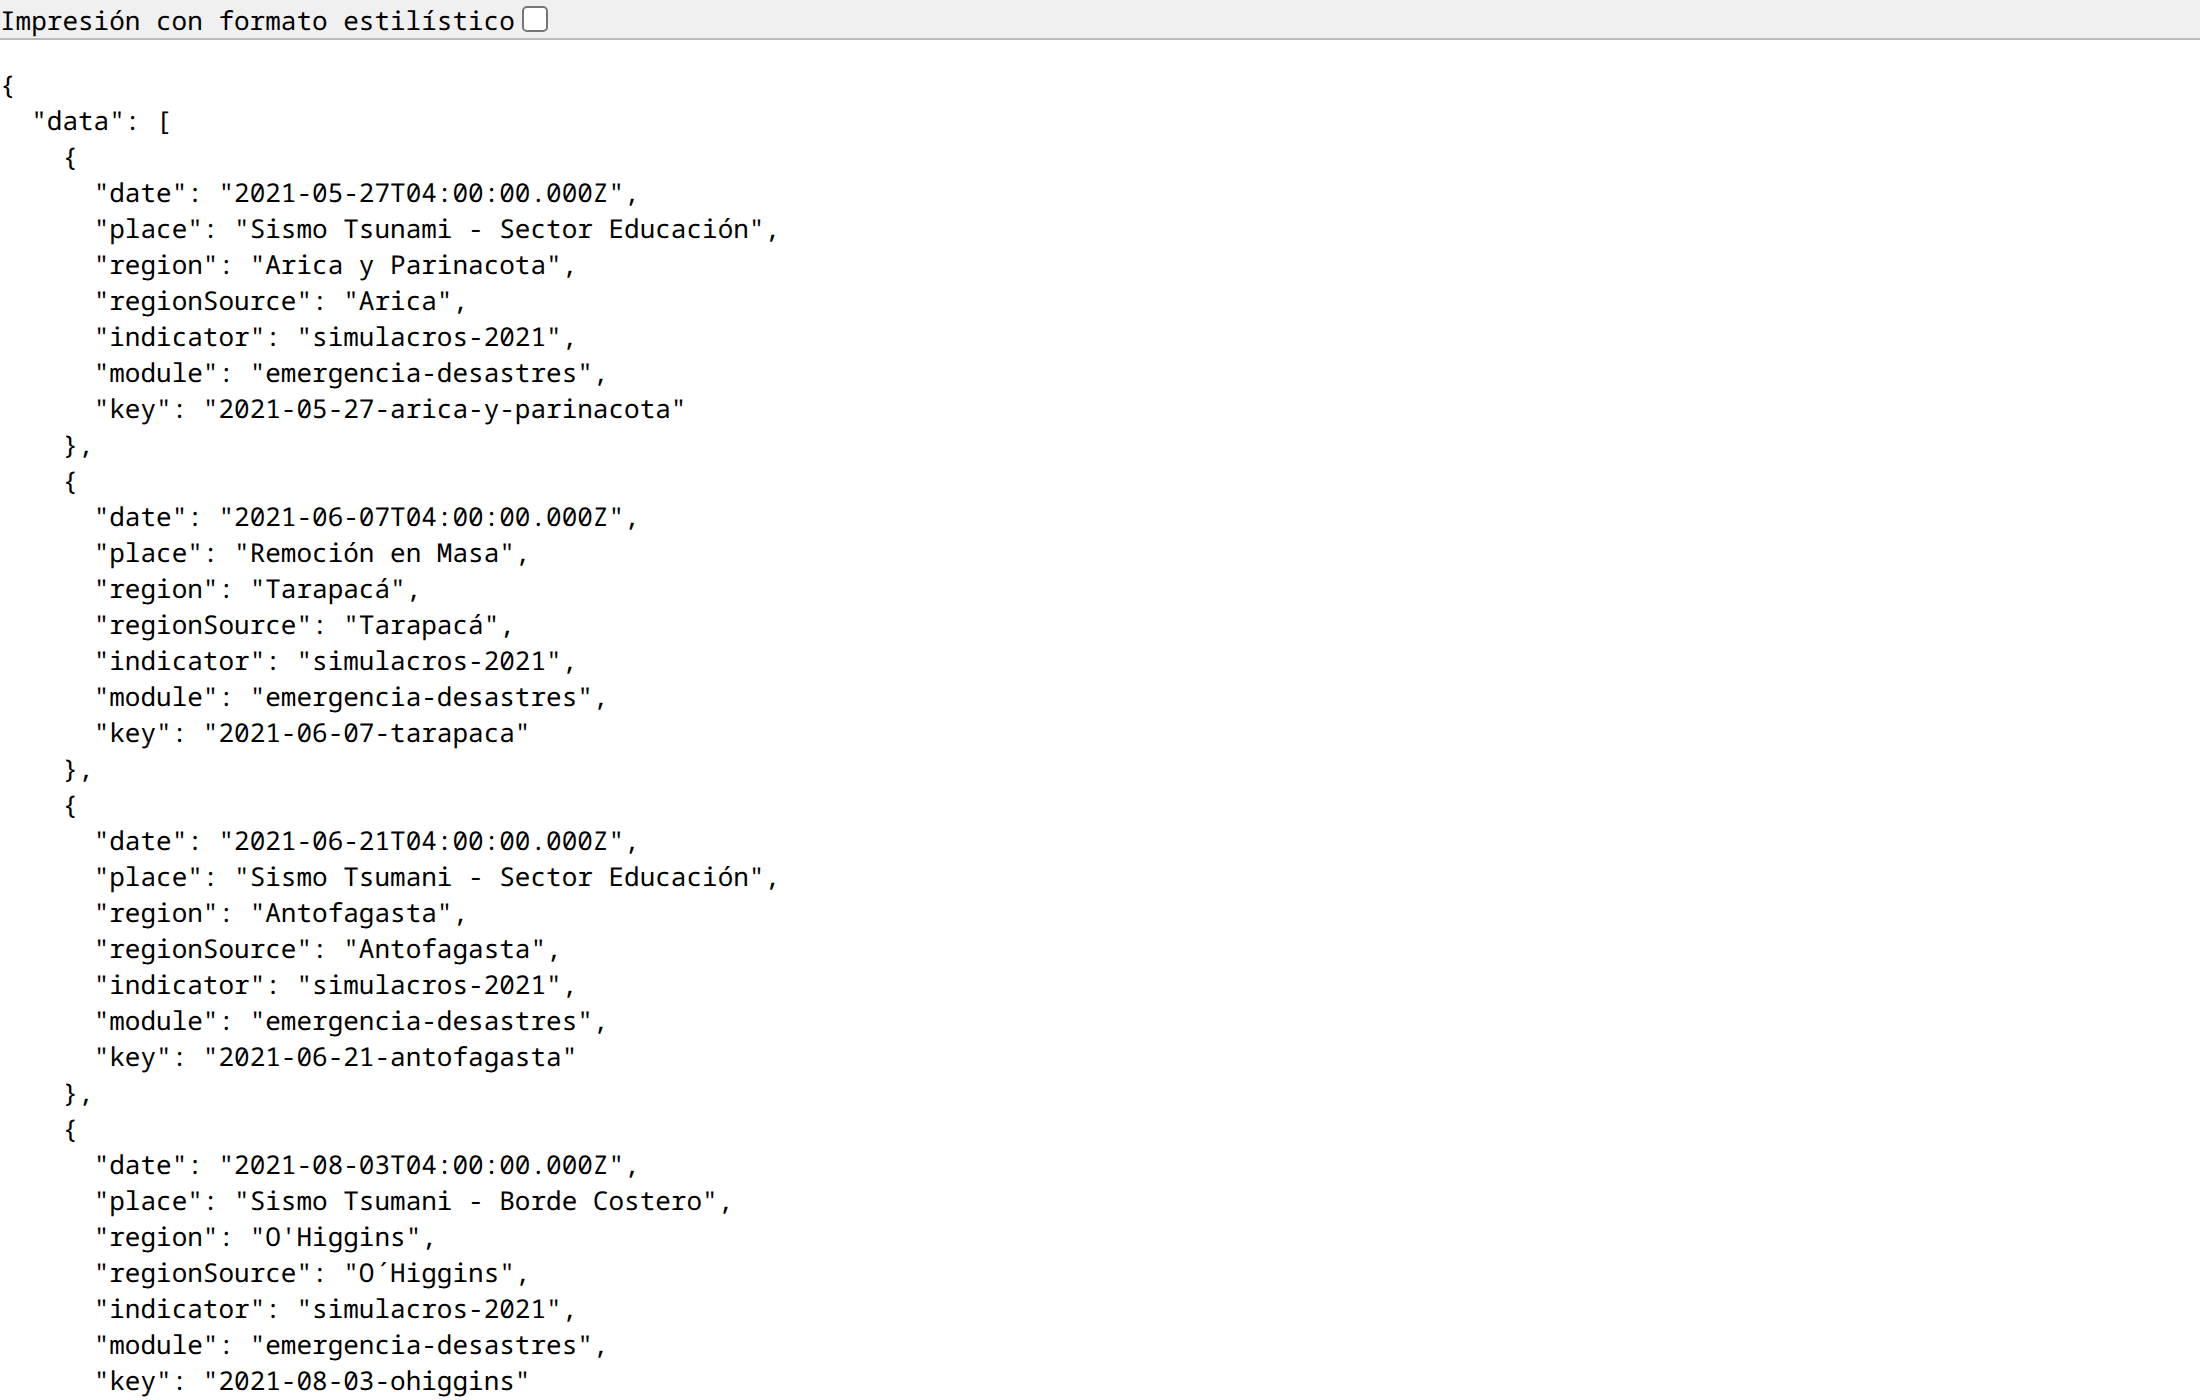
\includegraphics[width=0.92\textwidth]{img_15.png}
  \caption{Extracto de los registros de simulacros-2021 mostrando fecha, tipo y regi\'on}
  \label{fig:registros-simulacros}
\end{figure}

\subsection{Resultados calculados de Tsunami Drills}
\label{sec:resultado-calculator}

El \textit{CalculatorAdapter} proces\'o los datos extra\'idos y almacen\'o los resultados en la colecci\'on \texttt{indicator-results}:

\begin{table}[H]
\centering
\caption{Resultados calculados por indicador de simulacros}
\label{tab:resultados-calculados}
\begin{tabular}{|l|c|c|}
\hline
\textbf{Indicador} & \textbf{Total de simulacros} & \textbf{Regiones distintas} \\
\hline
simulacros-2021 & 9 & 9 \\
\hline
simulacros-2022 & 11 & 11 \\
\hline
simulacros-2023 & 9 & 9 \\
\hline
\end{tabular}
\end{table}

En los tres a\~nos cada regi\'on aparece una sola vez, por lo que el total de simulacros coincide con la cantidad de regiones distintas. La Figura~\ref{fig:api-resultado-calculado} muestra el resultado tal como lo entrega el \textit{endpoint} \texttt{GET /emergencia-desastres/simulacros-2021/result}.

\begin{figure}[H]
  \centering
  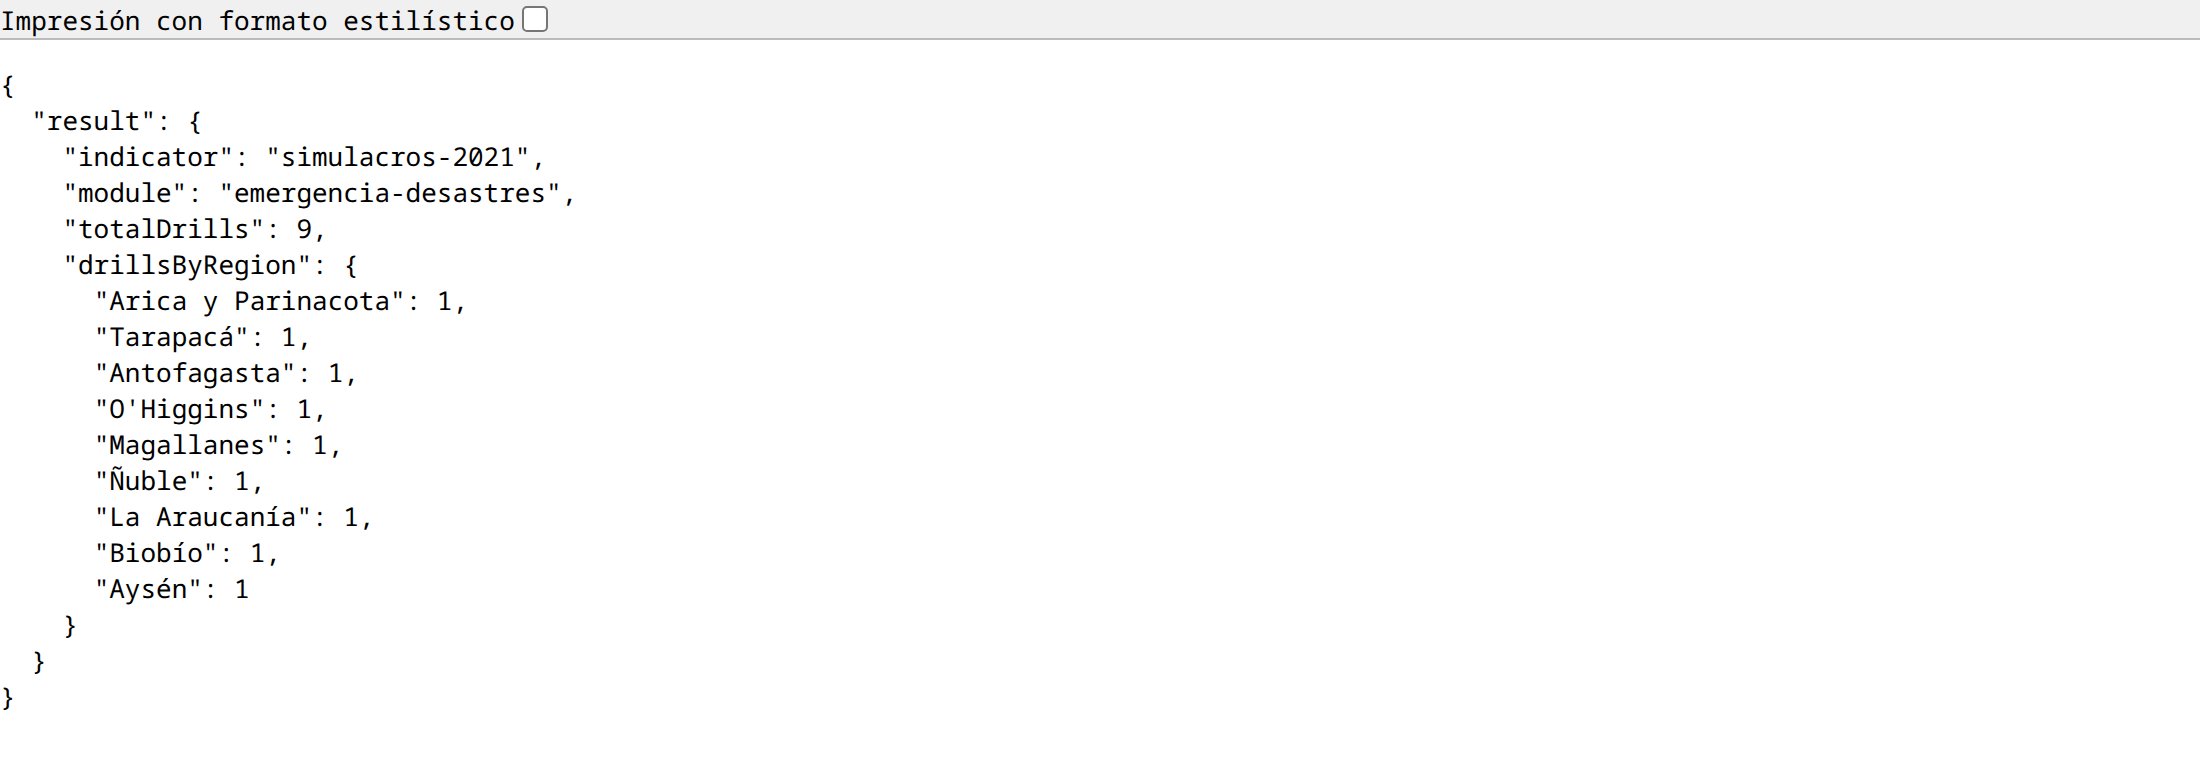
\includegraphics[width=0.92\textwidth]{img_16.png}
  \caption{Resultado calculado de simulacros-2021 consultado desde la API}
  \label{fig:api-resultado-calculado}
\end{figure}

Estos resultados permiten a los investigadores consultar de forma directa la cantidad de simulacros realizados por a\~no y su distribuci\'on geogr\'afica, sin necesidad de procesar los datos crudos manualmente. Las Figuras~\ref{fig:metabase-simulacros} y~\ref{fig:metabase-simulacros-region} presentan ambas lecturas en Metabase.

\begin{figure}[H]
  \centering
  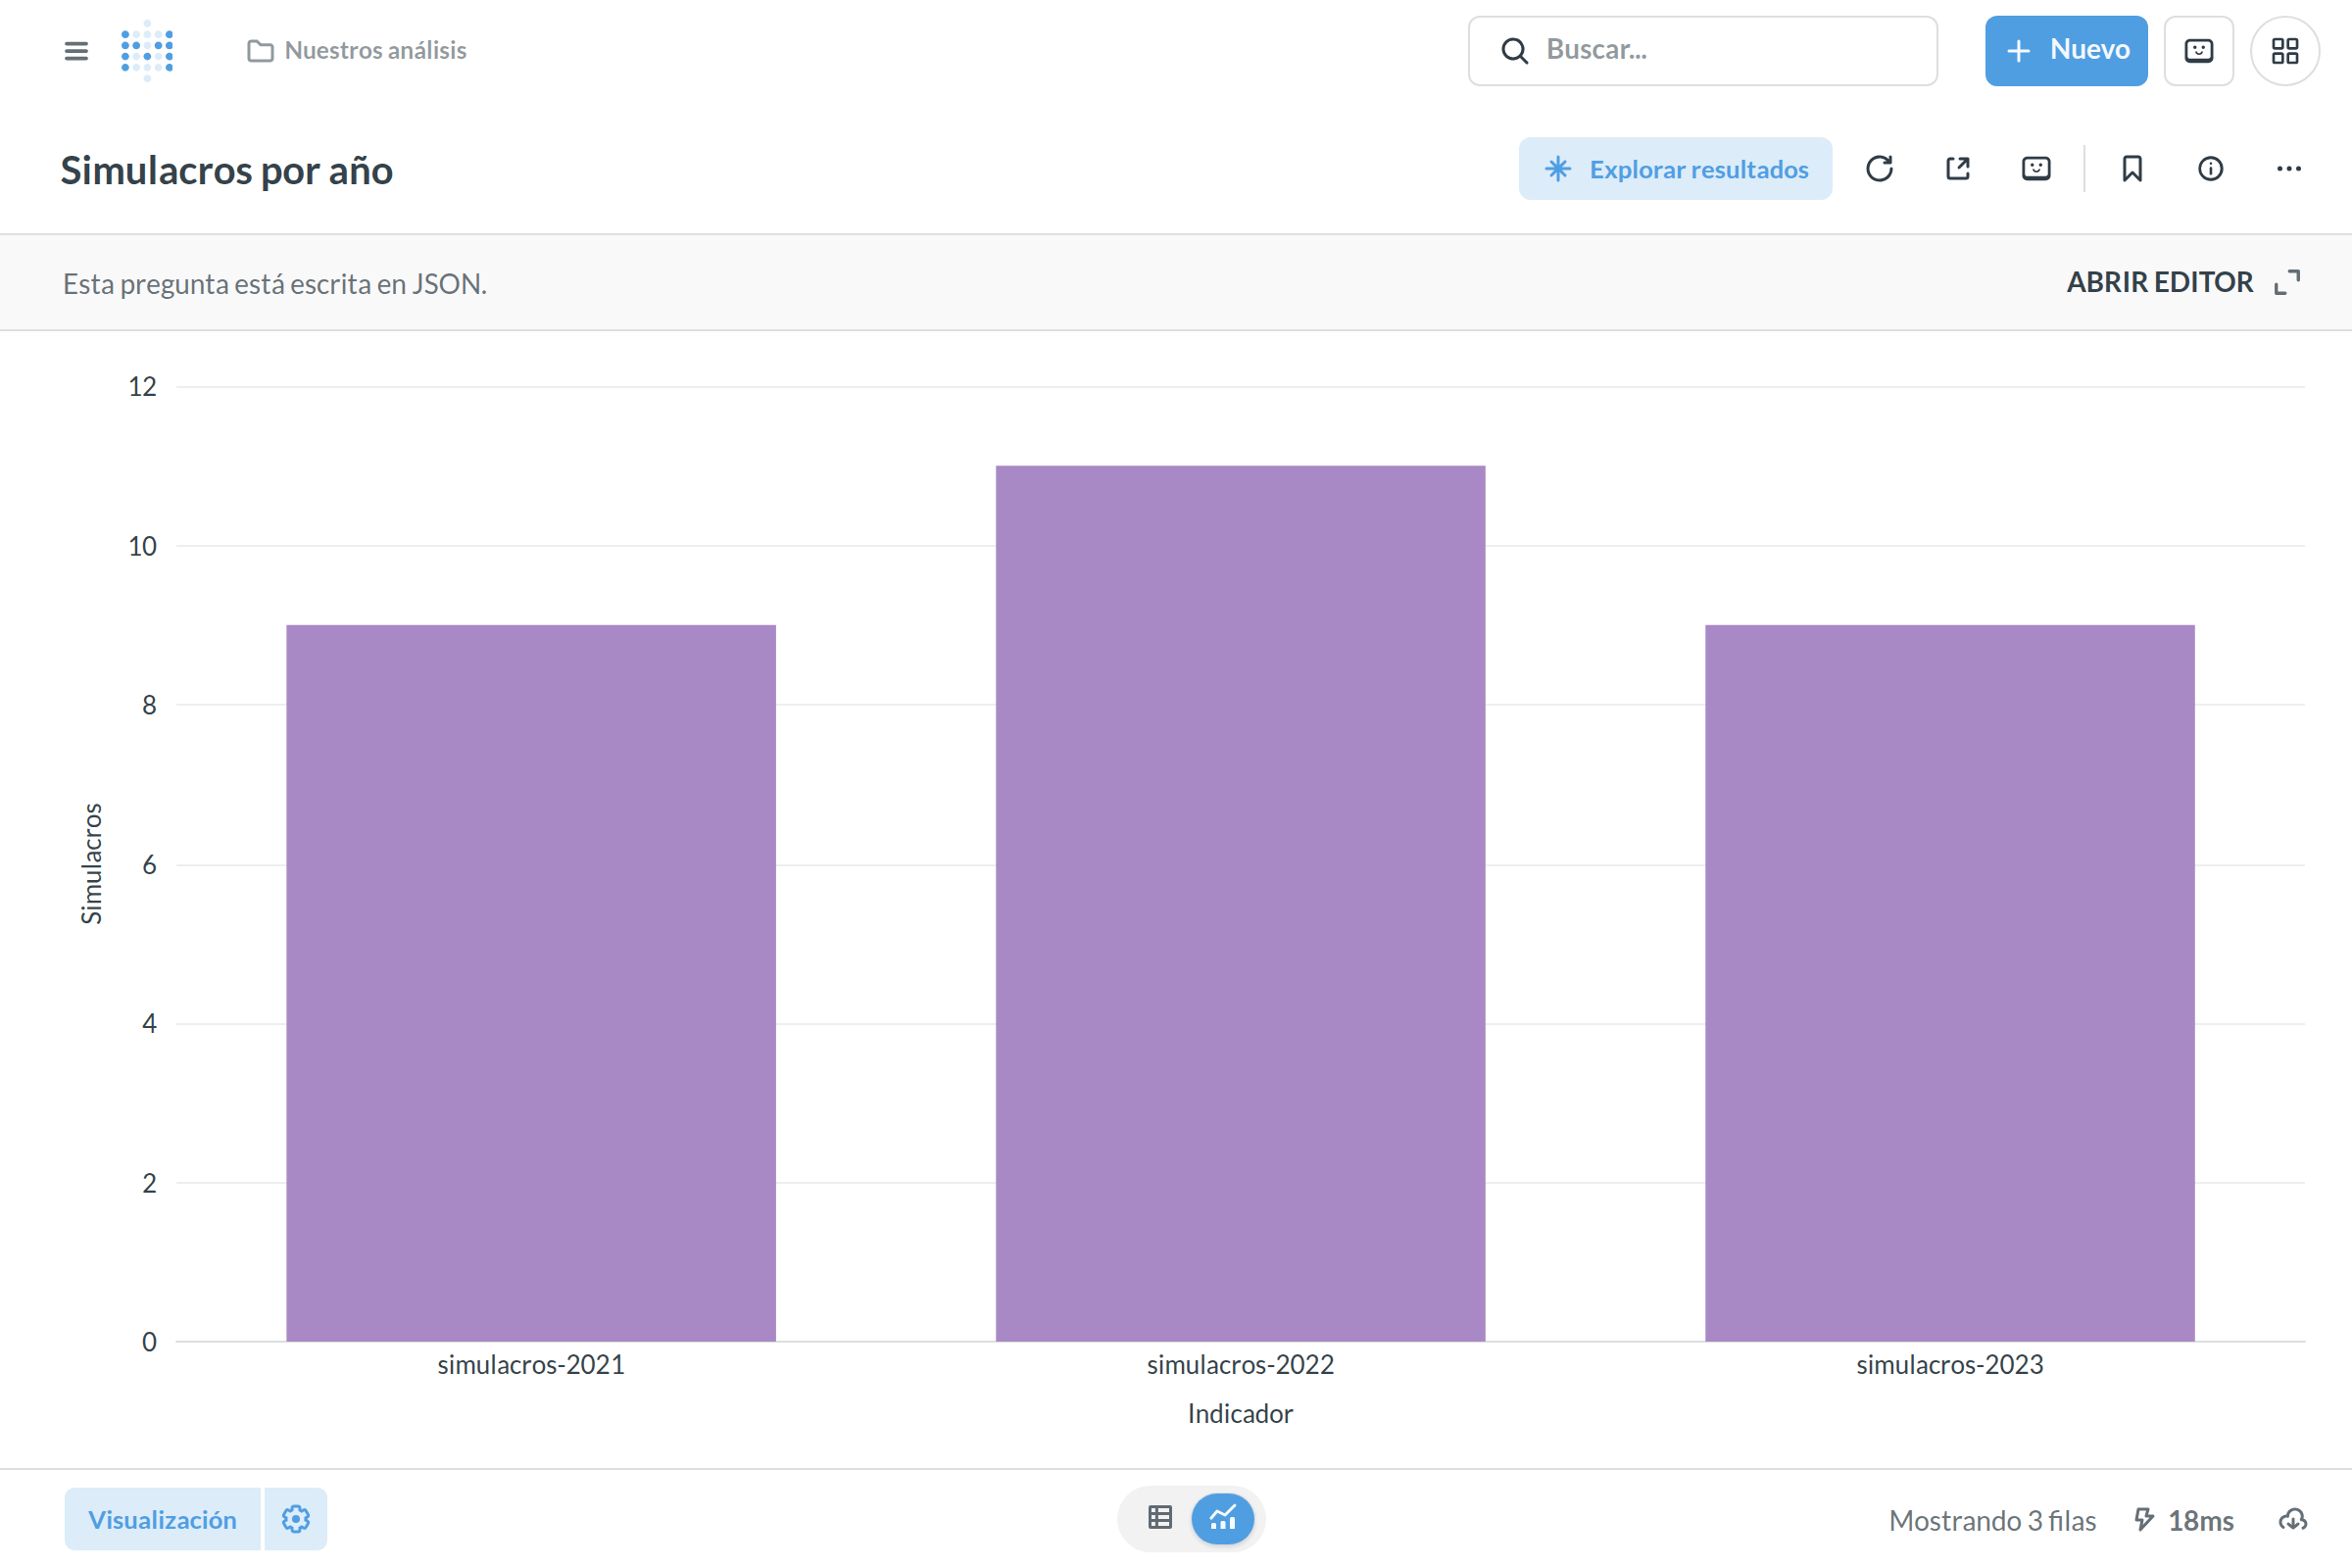
\includegraphics[width=0.8\textwidth]{img_19.png}
  \caption{Gr\'afico de barras de simulacros por a\~no en Metabase}
  \label{fig:metabase-simulacros}
\end{figure}

\begin{figure}[H]
  \centering
  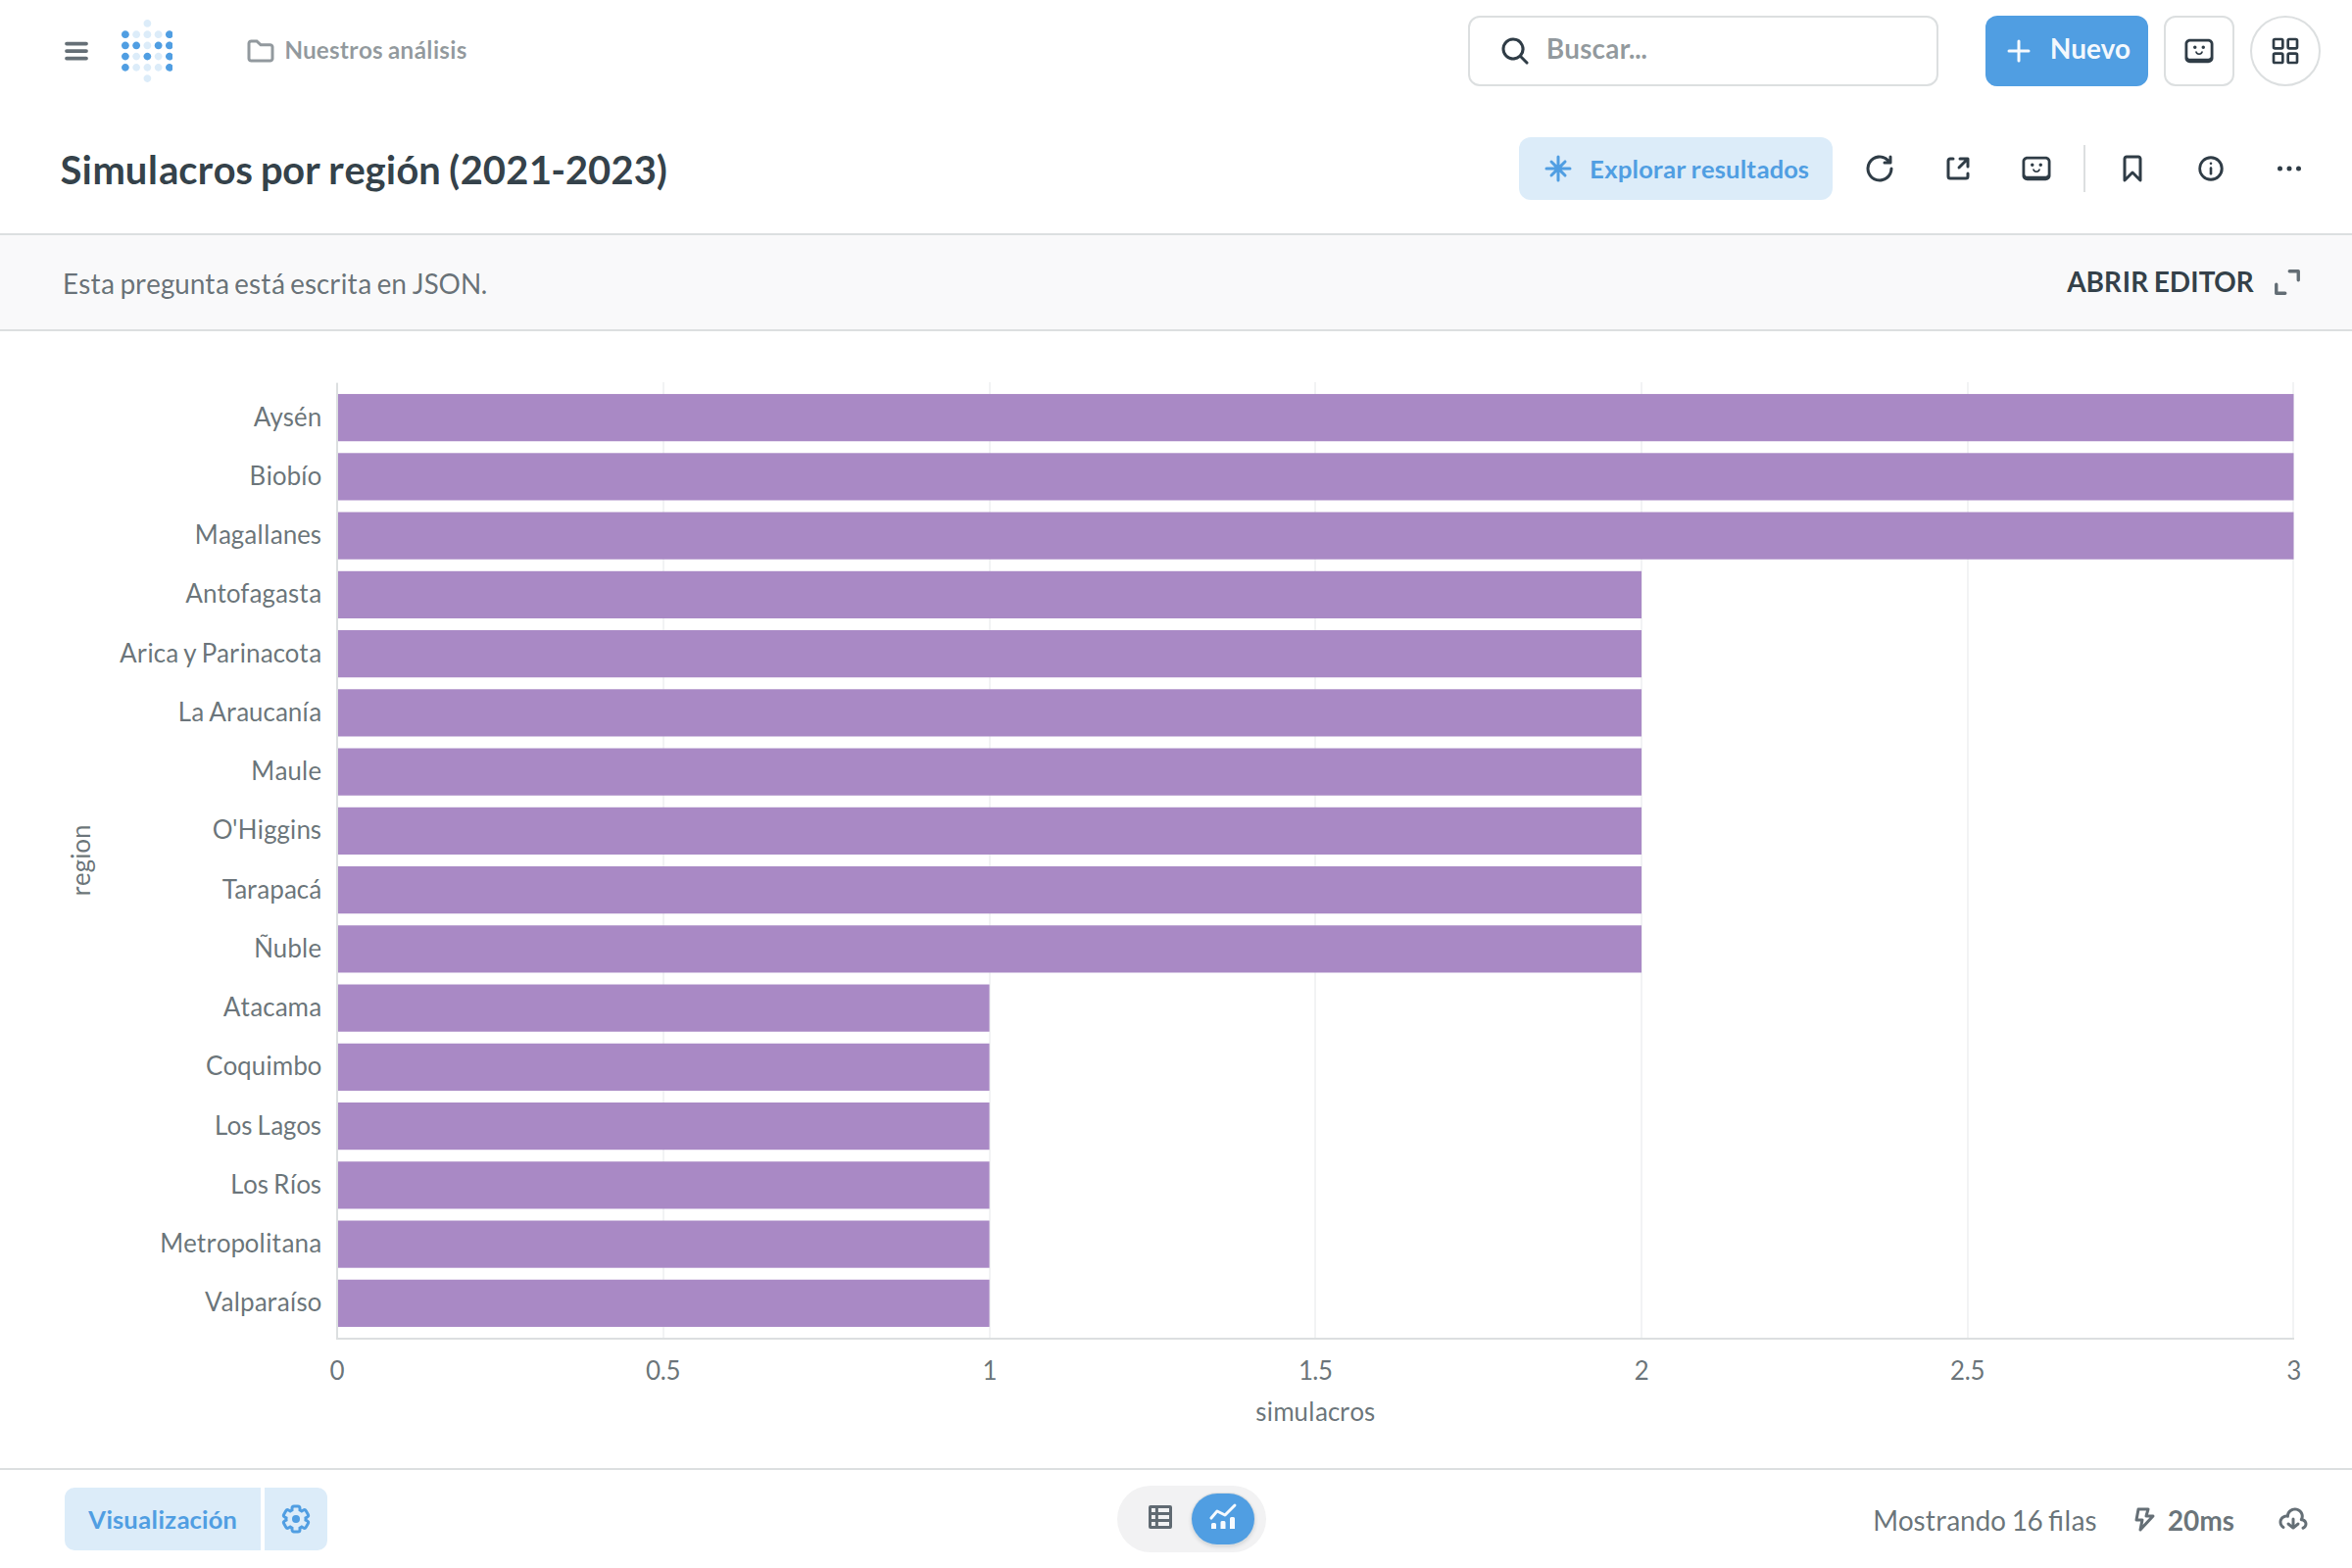
\includegraphics[width=0.8\textwidth]{img_20.png}
  \caption{Distribuci\'on acumulada de simulacros por regi\'on (2021-2023) en Metabase}
  \label{fig:metabase-simulacros-region}
\end{figure}

La agrupaci\'on se realiza sobre el campo \texttt{region} y no sobre \texttt{regionSource}: de lo contrario una misma regi\'on aparecer\'ia dividida en varias barras producto de las graf\'ias inconsistentes de la fuente.

\subsection{Tasa de Pobreza por Ingresos}
\label{sec:resultado-pobreza}

El sub-indicador \textit{tasa-pobreza-ingresos} extrajo tres registros correspondientes a la comuna de Valdivia, la Regi\'on de Los R\'ios y el pa\'is:

\begin{table}[H]
\centering
\caption{Datos extra\'idos de tasa de pobreza por ingresos}
\label{tab:pobreza}
\begin{tabular}{|l|c|c|}
\hline
\textbf{Unidad Territorial} & \textbf{CASEN 2017} & \textbf{CASEN 2022} \\
\hline
Comuna de Valdivia & 7,6\% & 3,4\% \\
\hline
Regi\'on de Los R\'ios & 11,8\% & 5,9\% \\
\hline
Pa\'is & 8,5\% & 6,5\% \\
\hline
\end{tabular}
\end{table}

Los porcentajes fueron convertidos correctamente del formato decimal chileno (con coma) al formato num\'erico est\'andar (con punto), permitiendo su uso directo en c\'alculos posteriores. La Figura~\ref{fig:api-pobreza} muestra la respuesta de la API y la Figura~\ref{fig:metabase-pobreza} la comparaci\'on entre ambas mediciones en Metabase.

\begin{figure}[H]
  \centering
  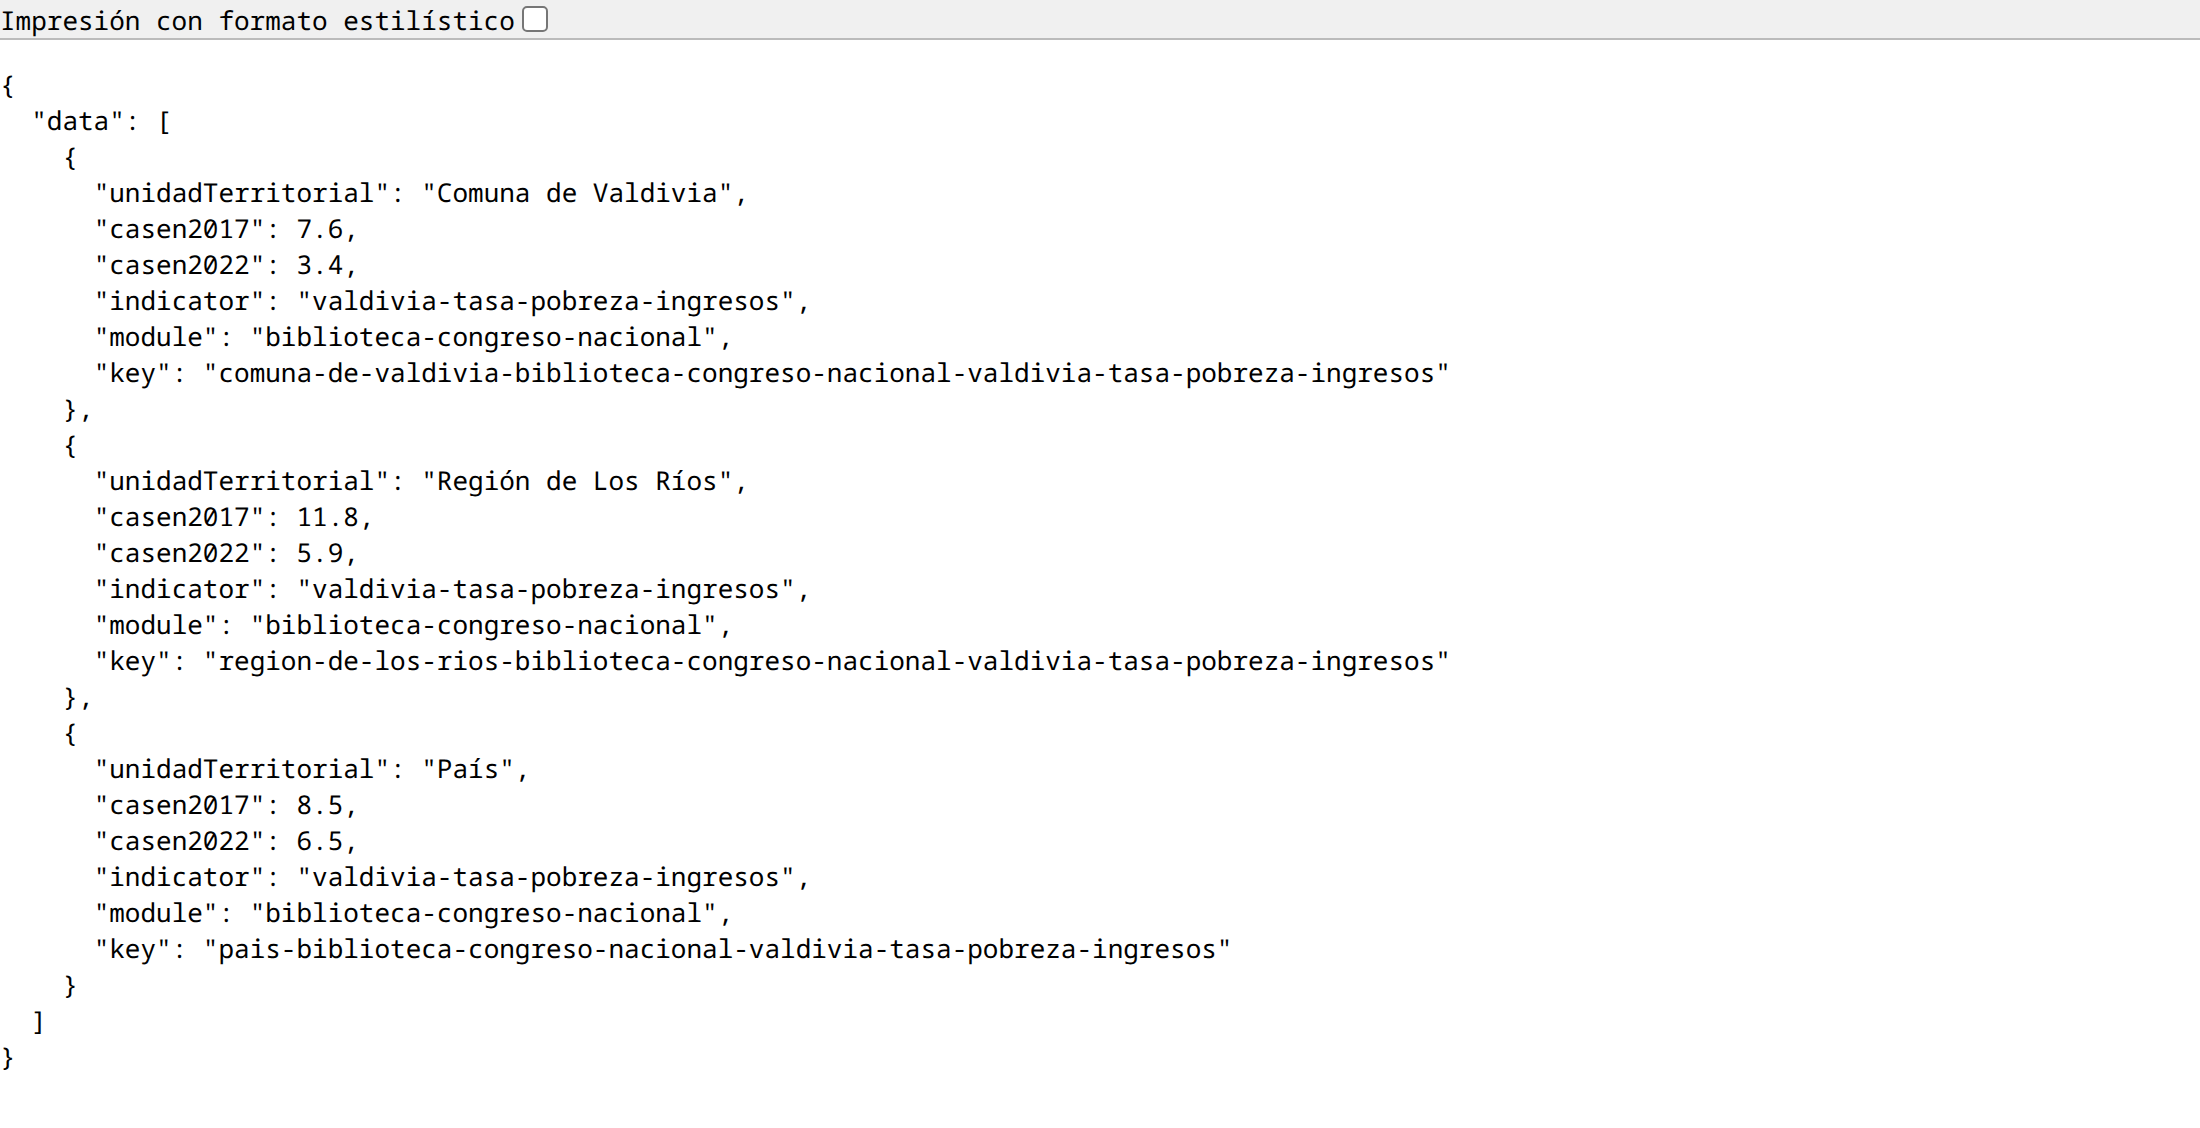
\includegraphics[width=0.92\textwidth]{img_17.png}
  \caption{Respuesta de la API para el indicador de tasa de pobreza por ingresos}
  \label{fig:api-pobreza}
\end{figure}

\begin{figure}[H]
  \centering
  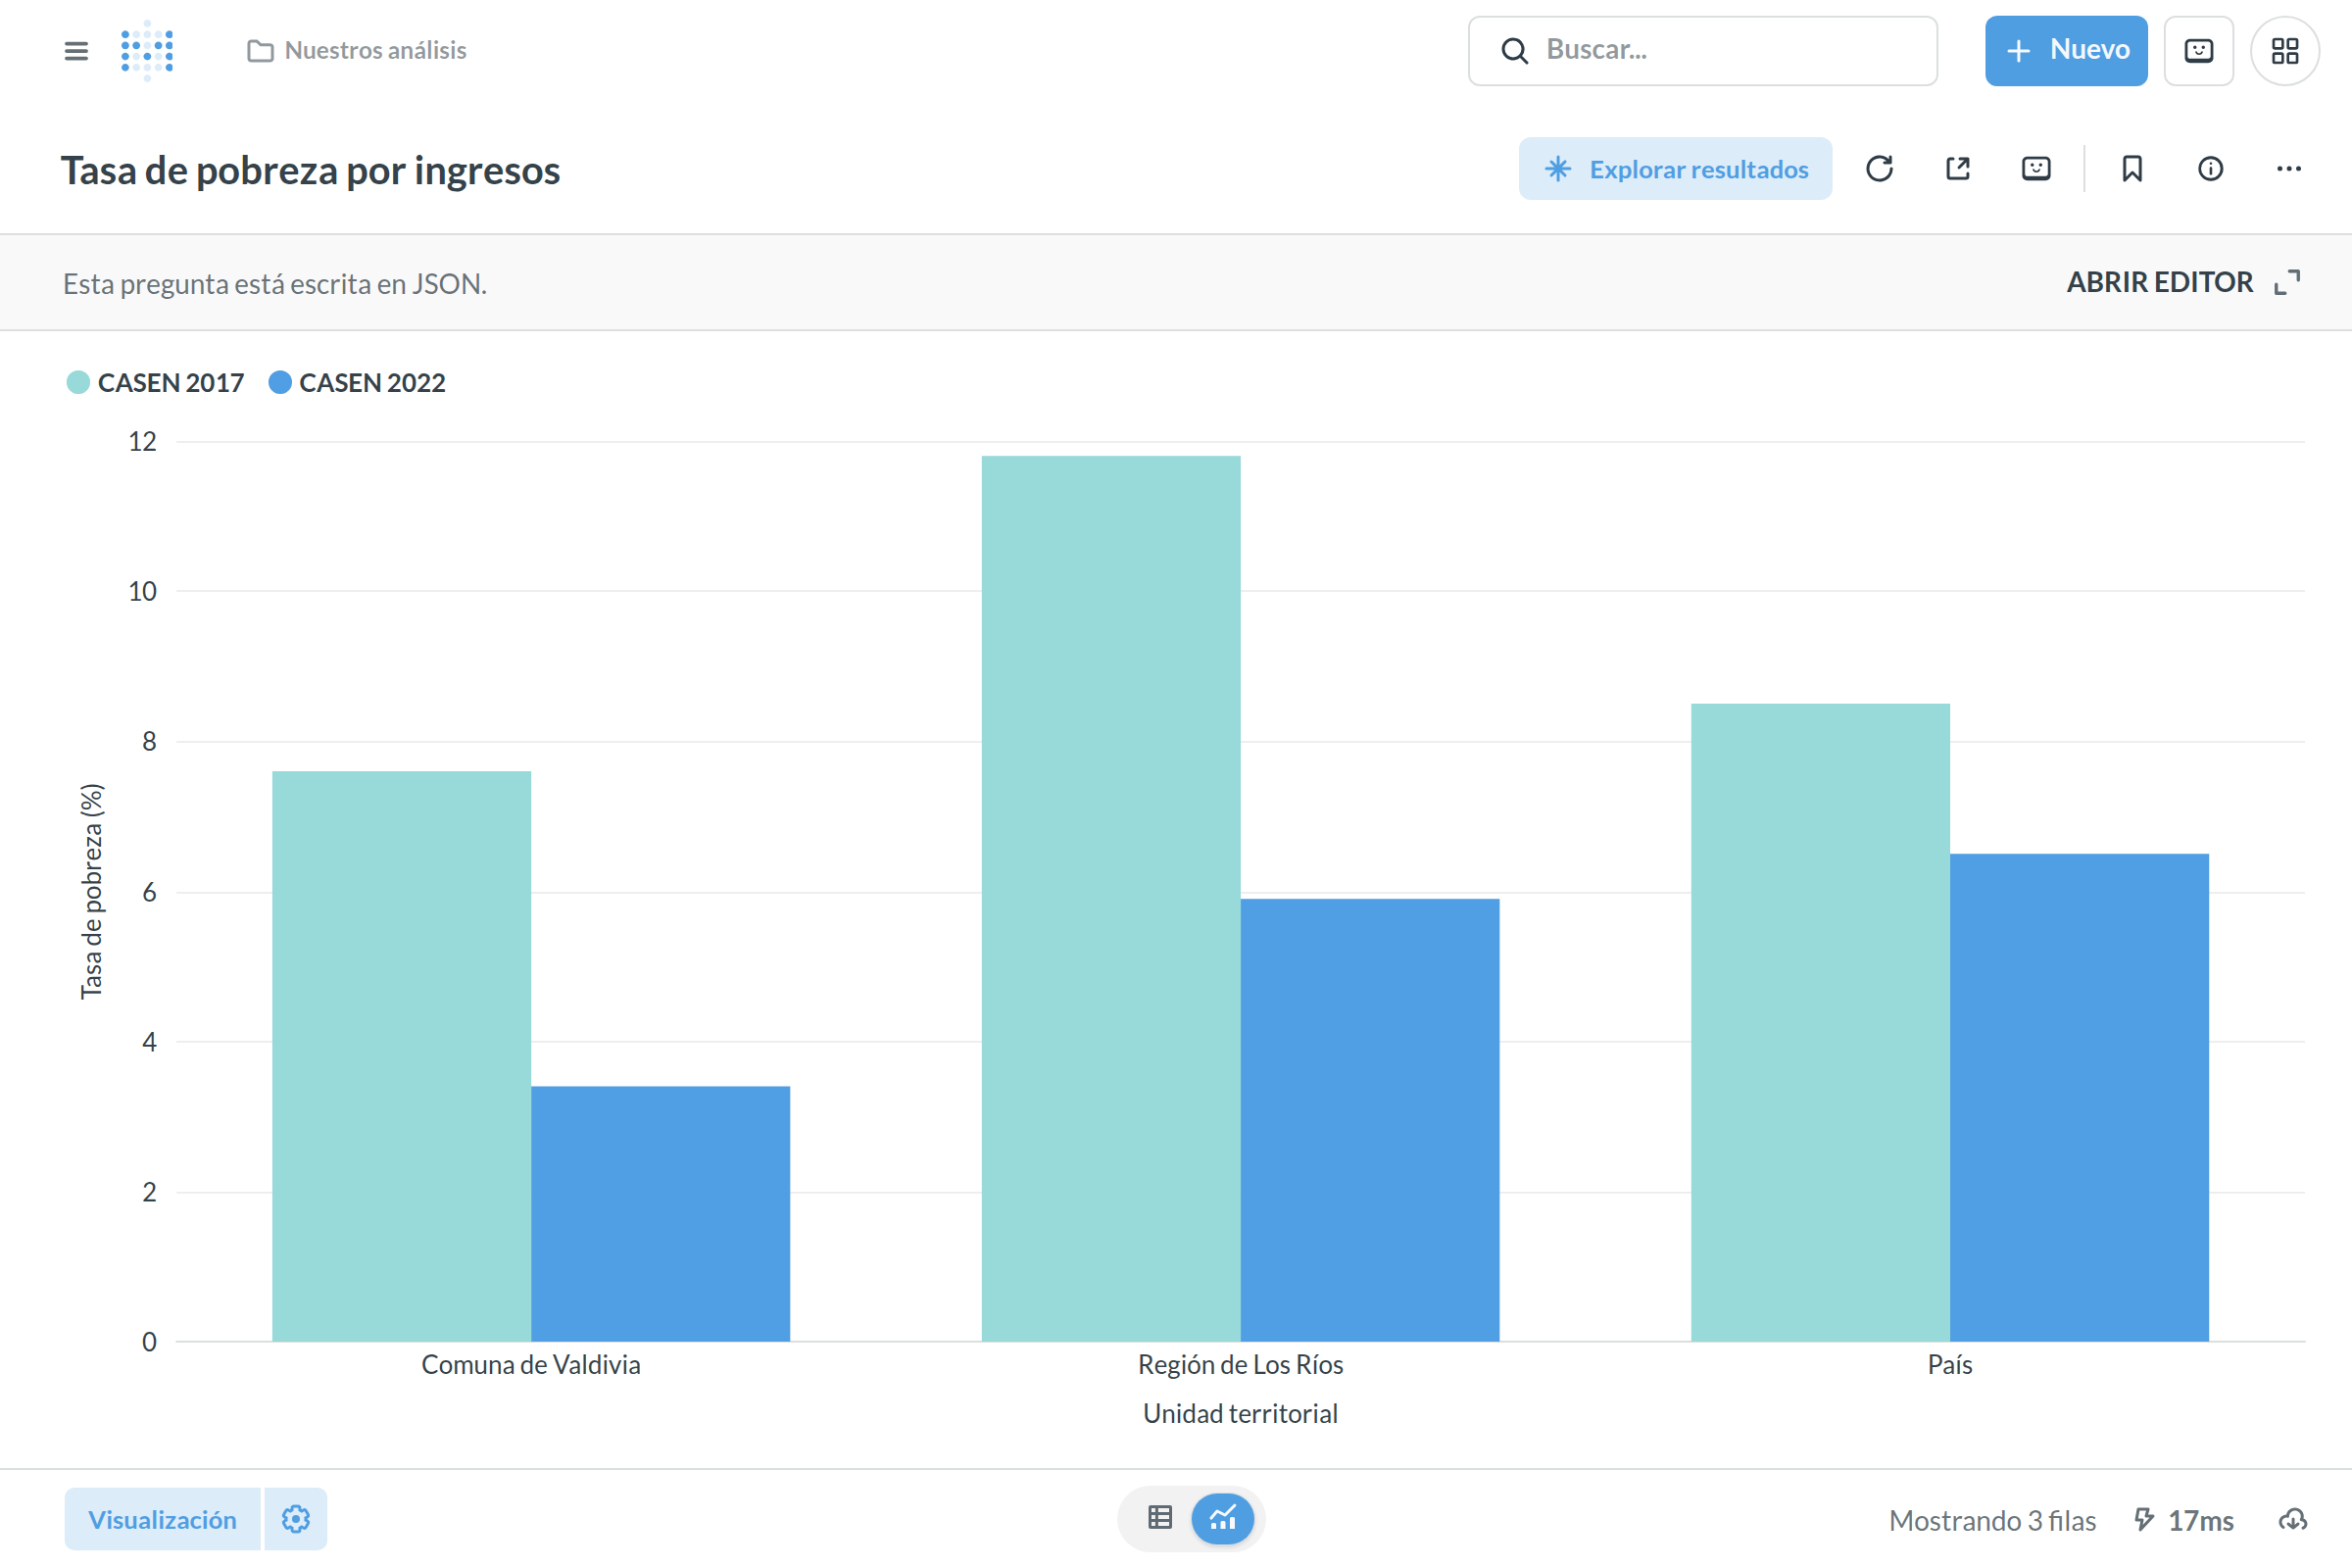
\includegraphics[width=0.8\textwidth]{img_21.png}
  \caption{Gr\'afico comparativo de pobreza CASEN 2017 frente a CASEN 2022 en Metabase}
  \label{fig:metabase-pobreza}
\end{figure}

\subsection{Organizaciones Comunitarias}
\label{sec:resultado-orgs}

El sub-indicador \textit{organizaciones-comunitarias} extrajo 17 registros correspondientes a los a\~nos 2008 a 2024 para la comuna de Valdivia. Cada registro contiene la cantidad de 11 tipos de organizaciones comunitarias: juntas de vecinos, clubes deportivos, centros de madres, centros culturales, centros del adulto mayor, uniones comunales, centros de padres y apoderados, compa\~n\'ias de bomberos, entre otros. La serie completa se presenta en la Figura~\ref{fig:metabase-organizaciones}.

\begin{figure}[H]
  \centering
  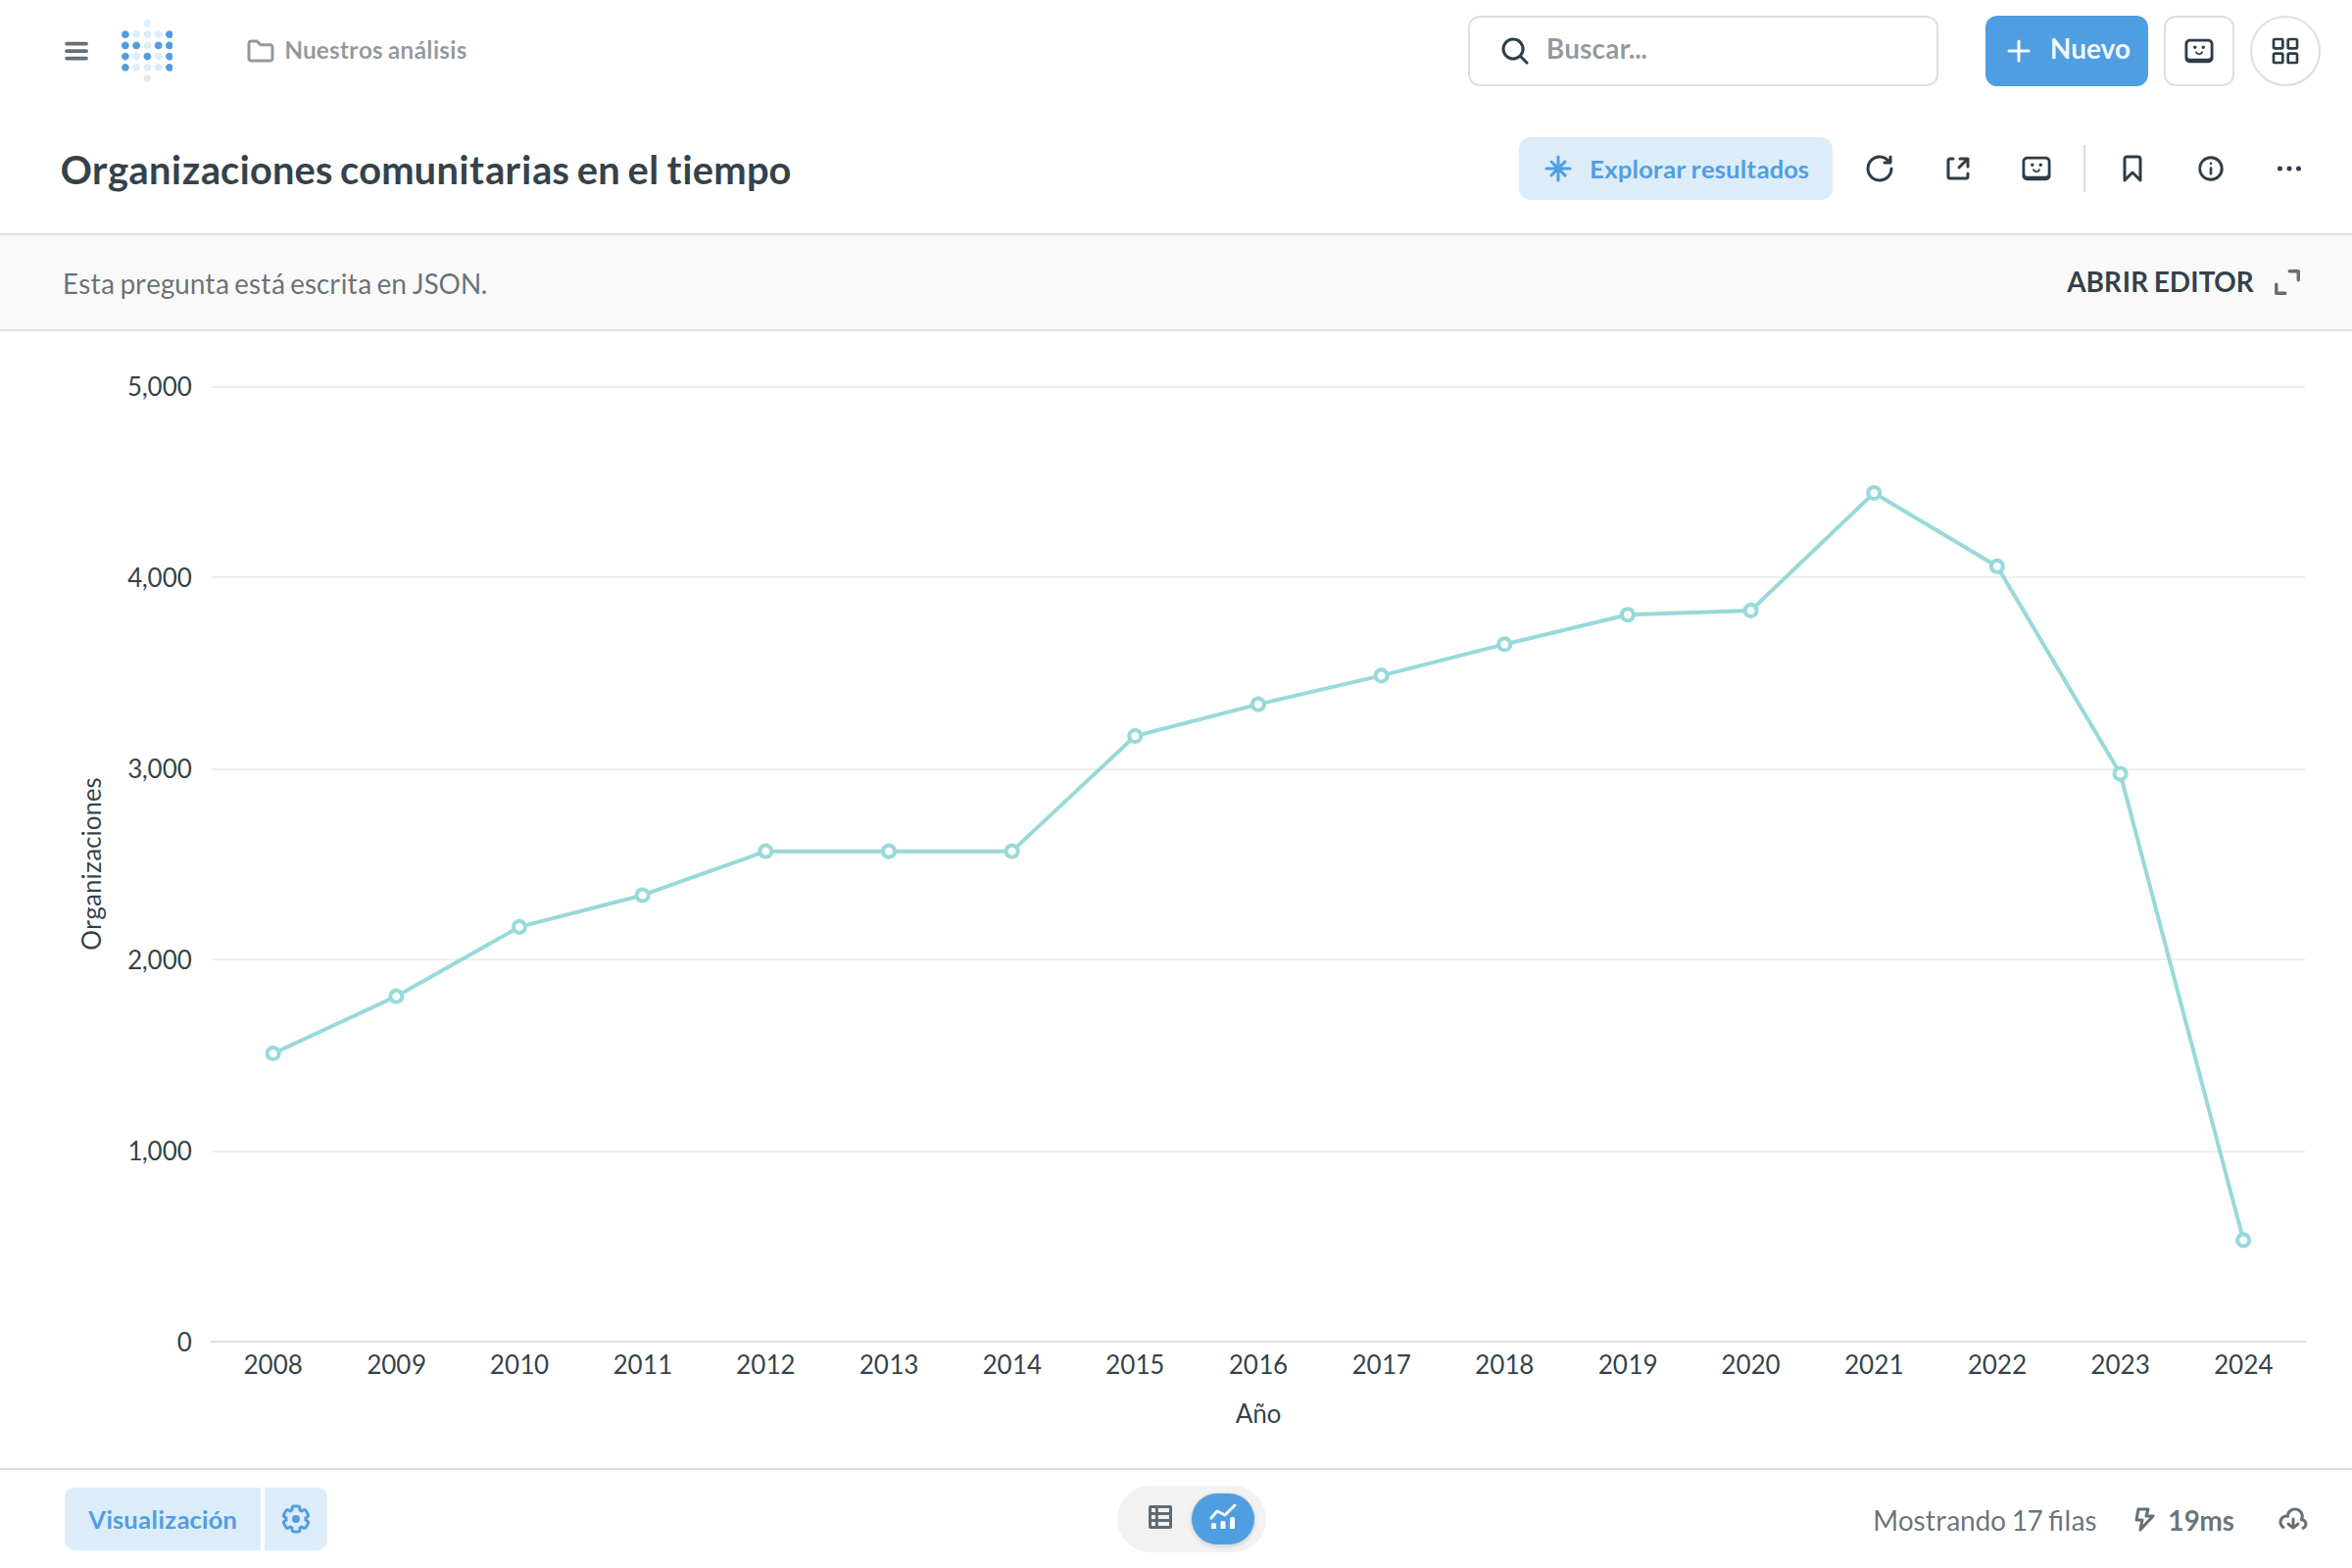
\includegraphics[width=0.85\textwidth]{img_22.png}
  \caption{Evoluci\'on temporal de las organizaciones comunitarias de Valdivia en Metabase}
  \label{fig:metabase-organizaciones}
\end{figure}

La construcci\'on de esta serie revel\'o una particularidad de la fuente que conviene explicitar. La BCN publica, adem\'as de la cantidad de cada tipo de organizaci\'on, un campo con la suma total; sin embargo, para algunos a\~nos ese campo viene informado con el car\'acter \texttt{-} en lugar de un n\'umero. El \textit{MapperAdapter} convierte esos valores a cero, lo que hace indistinguible un dato ausente de un cero real: en el a\~no 2017 la suma total qued\'o almacenada como cero pese a que los tipos individuales suman 3.485 organizaciones. Por esta raz\'on el gr\'afico recalcula el total a partir de los tipos individuales en lugar de utilizar el campo publicado por la fuente. La ca\'ida observada en el a\~no 2024 no responde a este problema, sino a que la fuente a\'un no publica todos los tipos para ese a\~no.

\section{La API REST en funcionamiento}
\label{sec:api-funcionamiento}

La API expone los indicadores mediante los \textit{endpoints} descritos en la Tabla~\ref{tab:endpoints}. El \textit{endpoint} ra\'iz act\'ua como punto de entrada y devuelve el cat\'alogo completo de m\'odulos e indicadores registrados en el \textit{ScraperFactory}, junto con la URL de la fuente y la frecuencia de actualizaci\'on de cada uno, tal como se aprecia en la Figura~\ref{fig:api-resumen}.

\begin{figure}[H]
  \centering
  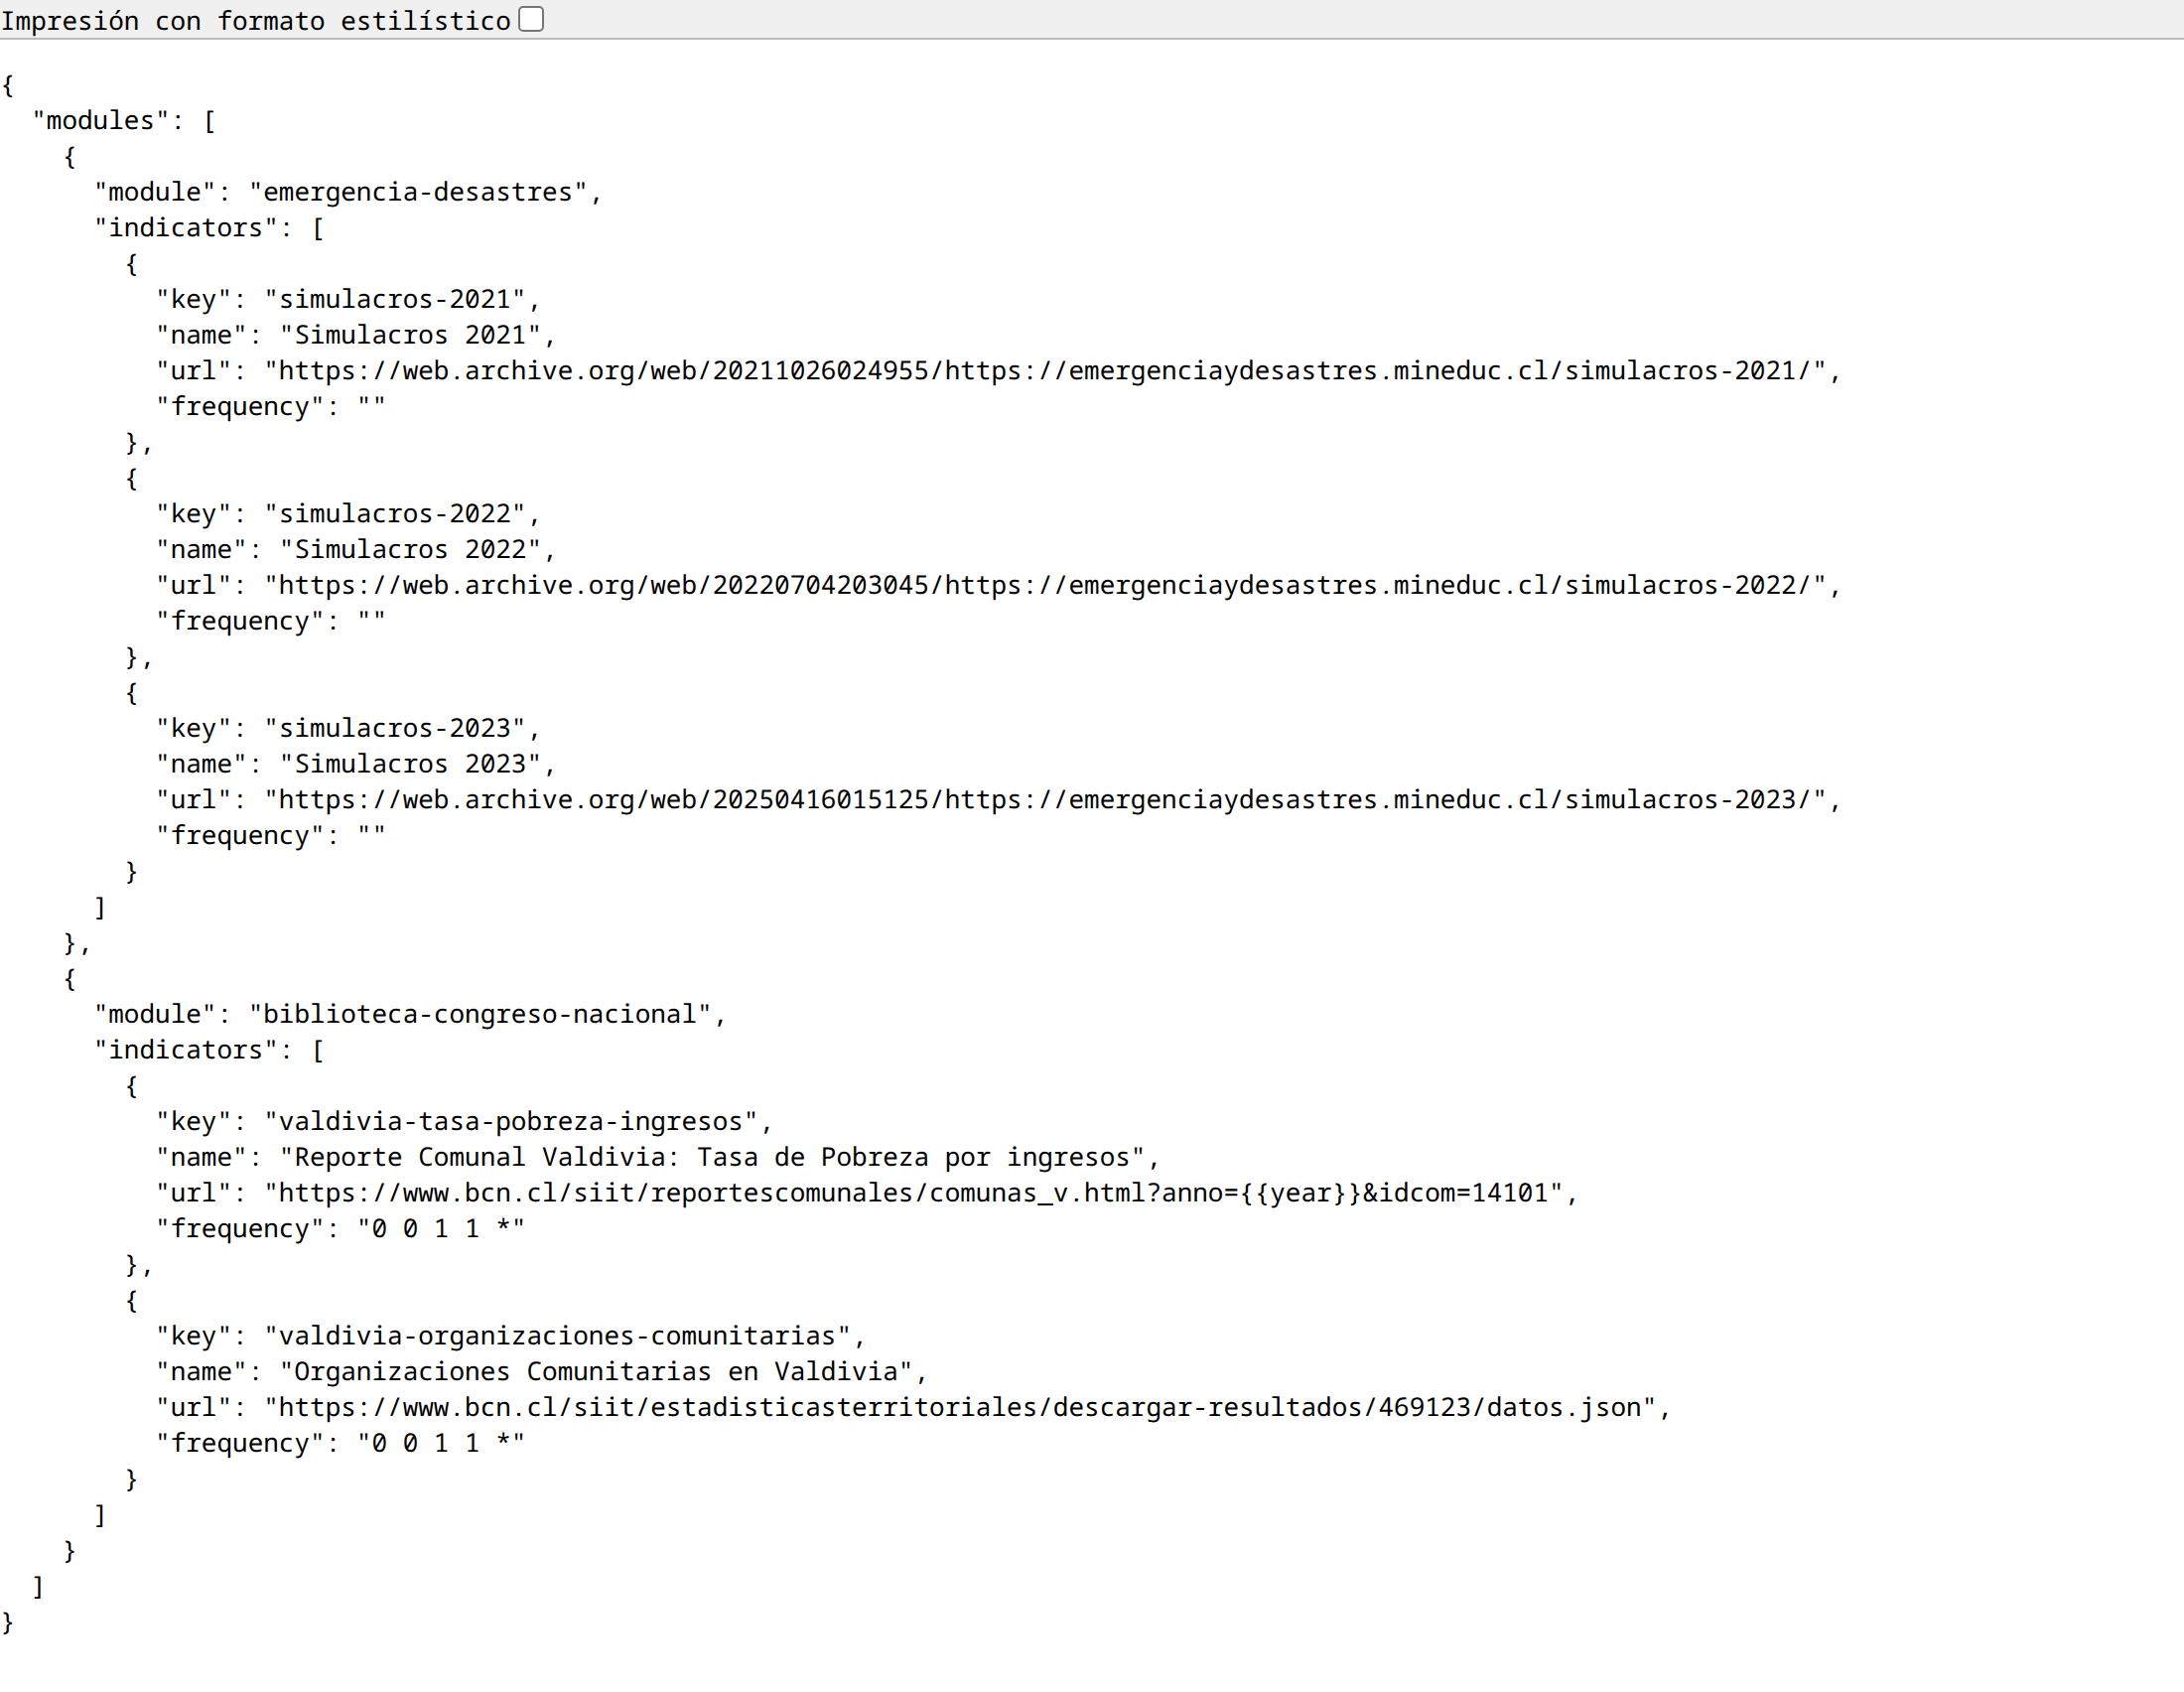
\includegraphics[width=0.92\textwidth]{img_14.png}
  \caption{Cat\'alogo de m\'odulos e indicadores devuelto por el \textit{endpoint} ra\'iz de la API}
  \label{fig:api-resumen}
\end{figure}

Este cat\'alogo se construye din\'amicamente a partir de los m\'odulos registrados, por lo que incorporar un nuevo indicador lo hace visible en la API sin modificar las rutas.

\section{Visualizaci\'on en Metabase}
\label{sec:visualizacion-resultados}

Los datos almacenados en MongoDB se visualizan mediante un \textit{dashboard} de Metabase que agrupa los cinco indicadores implementados (Figura~\ref{fig:metabase-dashboard}). Los gr\'aficos consultan directamente las colecciones, de modo que se actualizan de forma autom\'atica cada vez que el \textit{CronRegistry} ejecuta una extracci\'on.

\begin{figure}[H]
  \centering
  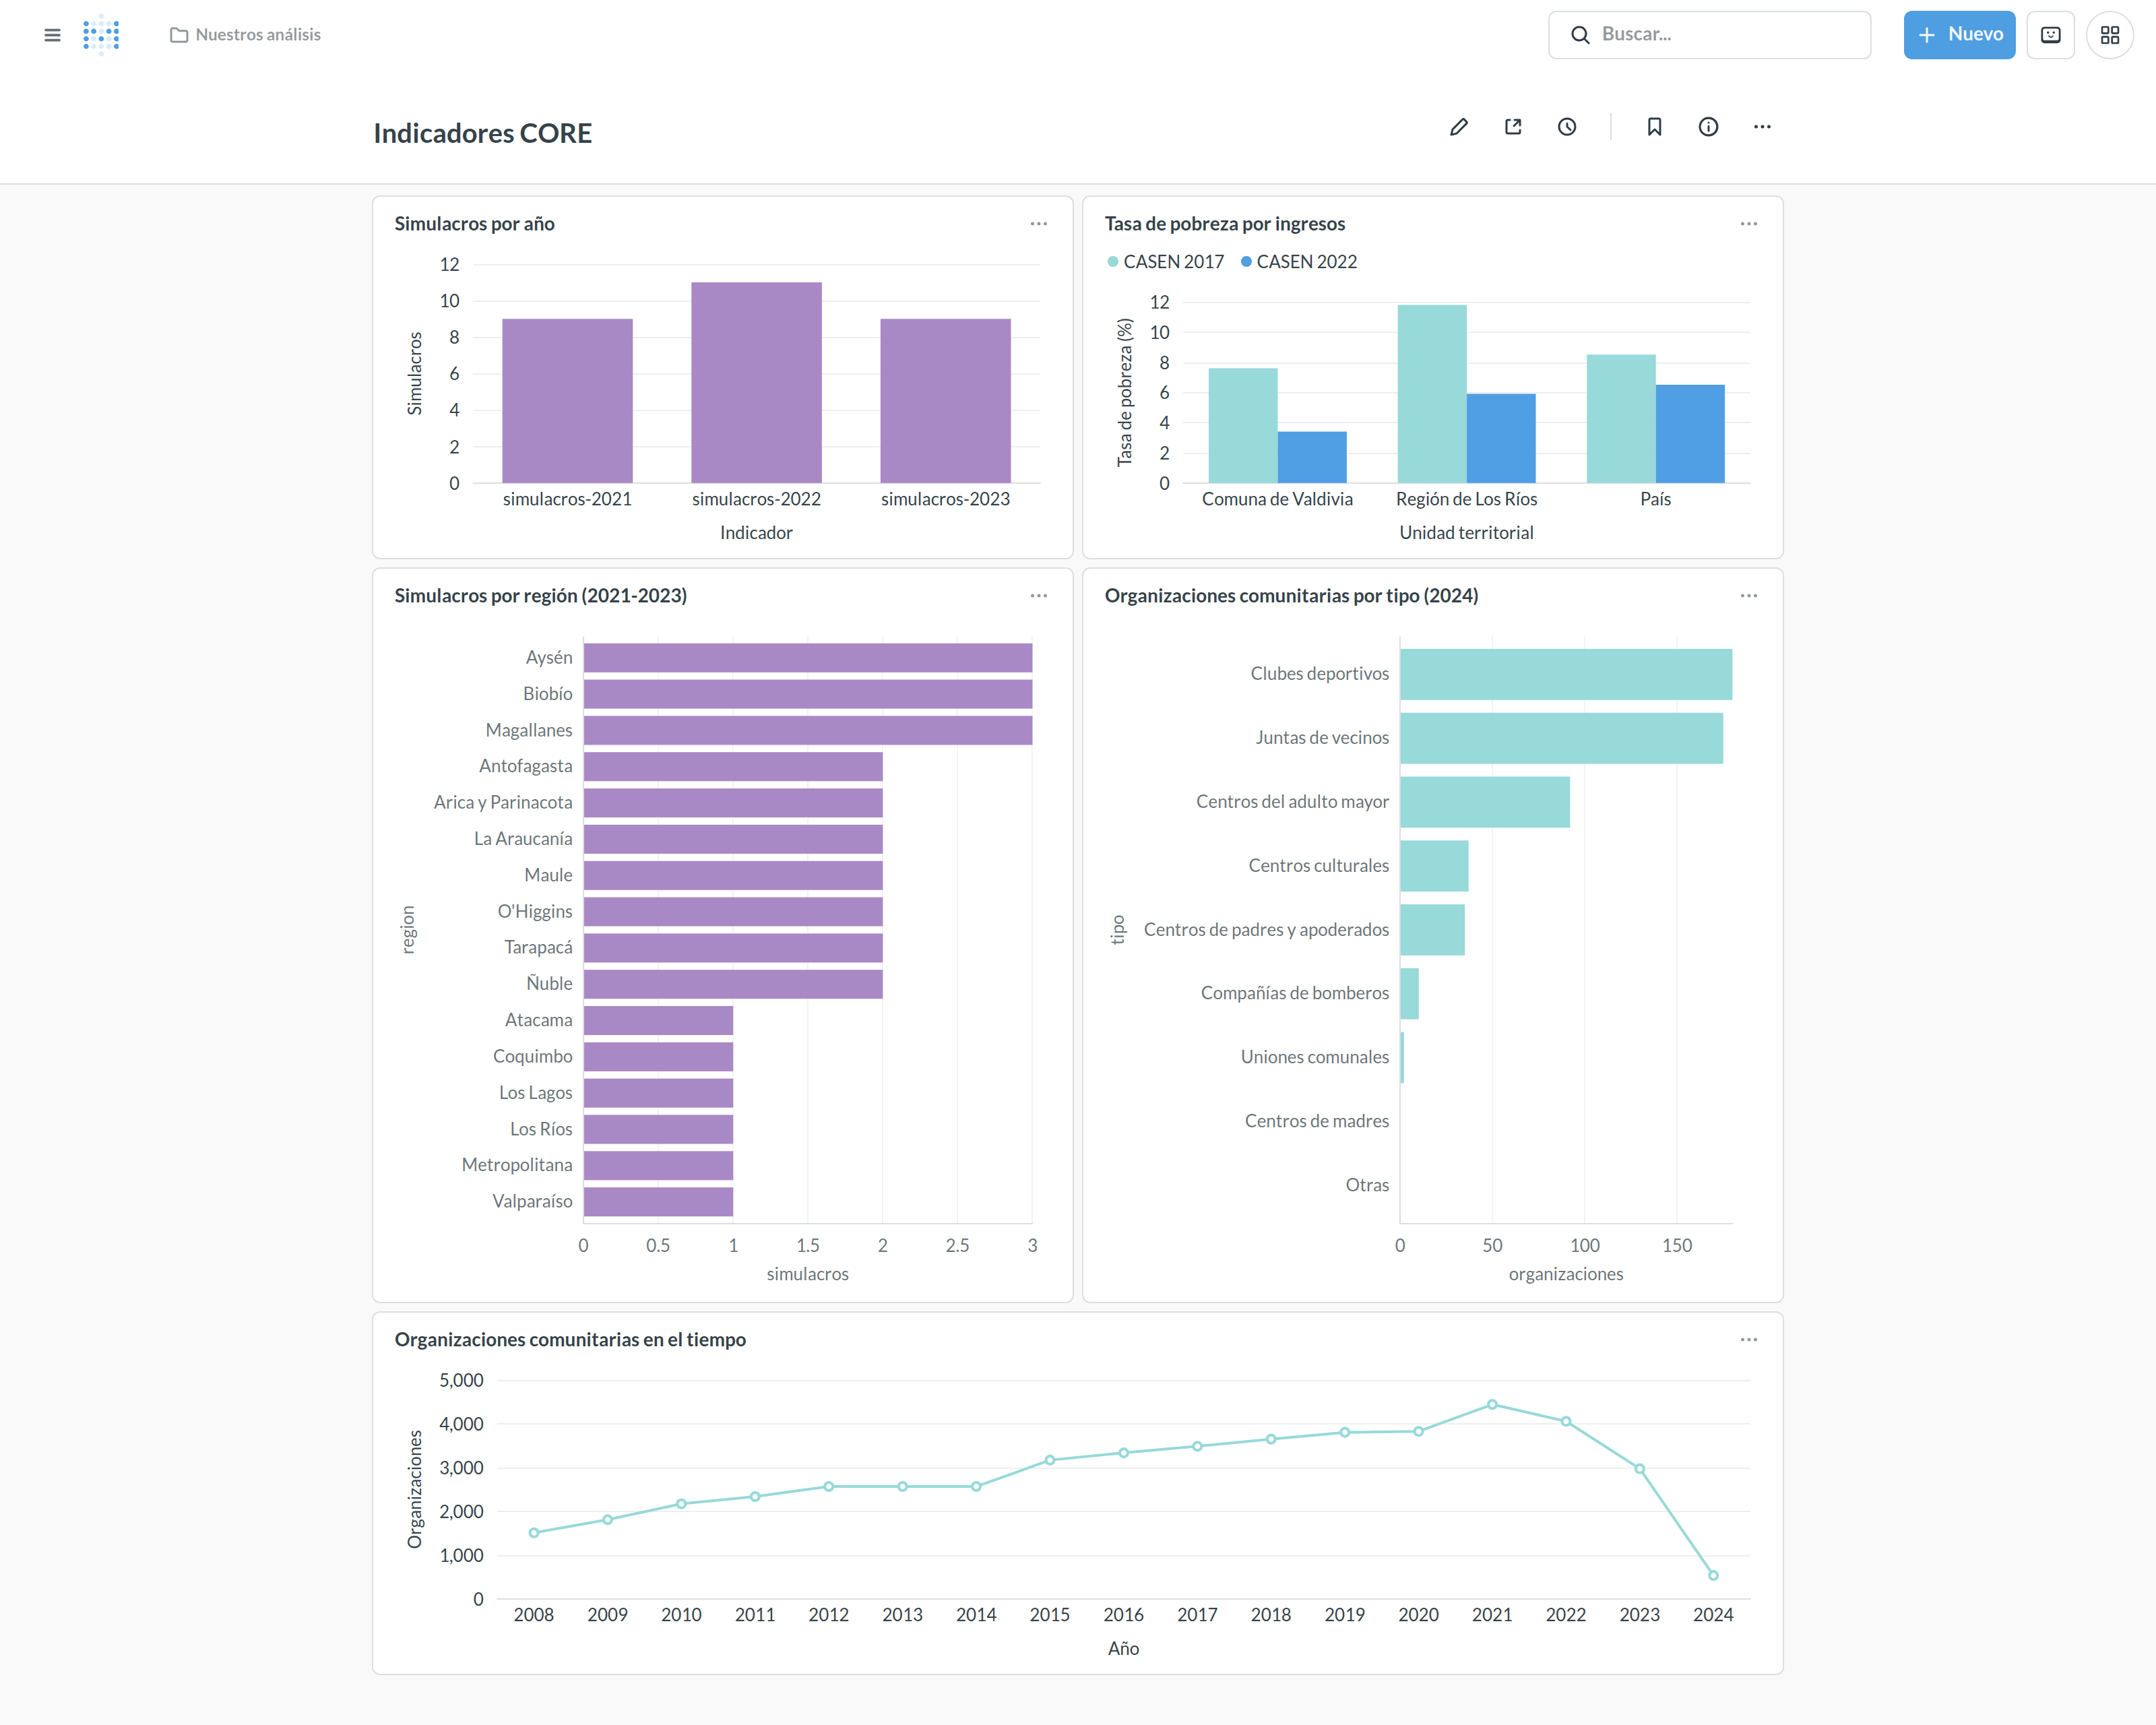
\includegraphics[width=\textwidth]{img_18.png}
  \caption{\textit{Dashboard} de Metabase con los indicadores del modelo CORE}
  \label{fig:metabase-dashboard}
\end{figure}

Tanto la conexi\'on a MongoDB como las consultas y el \textit{dashboard} se encuentran declarados en un archivo de configuraci\'on versionado junto al c\'odigo, y se aplican autom\'aticamente al levantar el entorno con Docker. De este modo la capa de anal\'itica es reproducible y no depende de una configuraci\'on manual de la herramienta.

\section{Validaci\'on de la extracci\'on}
\label{sec:validacion}

Para validar que los datos extra\'idos por el sistema son correctos, se realiz\'o una comparaci\'on con los valores le\'idos de forma manual en las mismas fuentes. La Tabla~\ref{tab:validacion} resume esta comparaci\'on.

\begin{table}[H]
\centering
\caption{Comparaci\'on entre los datos de referencia y los datos extra\'idos}
\label{tab:validacion}
\begin{tabular}{|l|l|c|c|}
\hline
\textbf{Indicador} & \textbf{Dato verificado} & \textbf{Fuente} & \textbf{Extra\'ido} \\
\hline
simulacros-2021 & Simulacros publicados & 9 & 9 \\
\hline
simulacros-2022 & Simulacros publicados & 11 & 11 \\
\hline
simulacros-2023 & Simulacros publicados & 9 & 9 \\
\hline
tasa-pobreza & Valdivia, CASEN 2017 & 7,6 & 7.6 \\
\hline
tasa-pobreza & Valdivia, CASEN 2022 & 3,4 & 3.4 \\
\hline
tasa-pobreza & Los R\'ios, CASEN 2017 & 11,8 & 11.8 \\
\hline
tasa-pobreza & Los R\'ios, CASEN 2022 & 5,9 & 5.9 \\
\hline
tasa-pobreza & Pa\'is, CASEN 2017 & 8,5 & 8.5 \\
\hline
tasa-pobreza & Pa\'is, CASEN 2022 & 6,5 & 6.5 \\
\hline
organizaciones & Suma total 2023 & 2.972 & 2972 \\
\hline
organizaciones & Suma total 2024 & 531 & 531 \\
\hline
\end{tabular}
\end{table}

En el caso de los simulacros, la verificaci\'on consisti\'o en contar las tarjetas publicadas en cada p\'agina archivada y contrastarlas con los registros almacenados. Adicionalmente se verific\'o que las fechas extra\'idas correspondieran a los meses correctos, considerando que la fuente utiliza abreviaciones en espa\~nol (Ene, Feb, Mar, entre otras); las pruebas automatizadas validan que cada abreviaci\'on sea convertida al \'indice de mes correcto.

En el caso de la tasa de pobreza se compararon los seis valores publicados en la tabla ``2.1 Tasa de Pobreza por ingresos'' del reporte comunal de la BCN con los almacenados en la base de datos. La \'unica diferencia es de formato: la fuente utiliza coma decimal y el sistema almacena punto decimal, conversi\'on que tambi\'en se encuentra cubierta por las pruebas automatizadas.

En el caso de las organizaciones comunitarias se verific\'o que la suma total publicada por la BCN coincidiera con la suma de los tipos individuales extra\'idos por el sistema. La coincidencia se cumple en todos los a\~nos en que la fuente informa dicho campo; los a\~nos en que la fuente lo entrega vac\'io se discuten en la secci\'on~\ref{sec:resultado-orgs}.

\section{Evitaci\'on de duplicados}
\label{sec:duplicados}

El sistema fue ejecutado m\'ultiples veces sobre las mismas fuentes de datos para verificar que los mecanismos de evitaci\'on de duplicados funcionaran correctamente. El \textit{HashAdapter} genera una clave \'unica para cada registro (basada en la fecha y la regi\'on para simulacros, en la unidad territorial para pobreza, y en el a\~no para organizaciones), y los esquemas de MongoDB declaran este campo como \'unico. En cada ejecuci\'on posterior a la primera, el sistema detect\'o los duplicados y los ignor\'o sin generar errores.

De manera similar, el \textit{CalculatorAdapter} compar\'o los resultados calculados con el \'ultimo resultado almacenado y no cre\'o registros nuevos cuando los datos de origen no hab\'ian cambiado.

\section{Rendimiento de la extracci\'on}
\label{sec:rendimiento}

Se instrument\'o el flujo ETL para medir el tiempo de cada etapa por separado. La Tabla~\ref{tab:rendimiento} presenta los tiempos obtenidos al ejecutar los cinco indicadores sobre colecciones vac\'ias, es decir, en el escenario en que todos los registros deben insertarse.

\begin{table}[H]
\centering
\caption{Tiempos de ejecuci\'on por etapa del flujo ETL, en milisegundos}
\label{tab:rendimiento}
\begin{tabular}{|l|c|c|c|c|c|c|}
\hline
\textbf{Indicador} & \textbf{Reg.} & \textbf{Fetch} & \textbf{Parse} & \textbf{Transf.} & \textbf{Save} & \textbf{Total} \\
\hline
simulacros-2021 & 9 & 881,1 & 42,2 & 1,3 & 13,4 & 947,6 \\
\hline
simulacros-2022 & 11 & 172,9 & 14,4 & 0,4 & 4,0 & 194,3 \\
\hline
simulacros-2023 & 9 & 172,0 & 11,4 & 0,3 & 3,5 & 192,7 \\
\hline
tasa-pobreza-ingresos & 3 & 333,8 & 38,5 & 0,3 & 3,0 & 375,5 \\
\hline
organizaciones-comunitarias & 17 & 121,6 & 0,1 & 0,5 & 8,3 & 130,3 \\
\hline
\end{tabular}
\end{table}

La columna \textit{Total} incluye adem\'as la etapa de c\'alculo, presente solo en los indicadores de simulacros. El tiempo mayor del primer indicador se explica por el costo inicial de establecer la conexi\'on HTTP y no por la cantidad de registros: en una segunda ejecuci\'on ese mismo indicador baj\'o a 182,4 ms.

La lectura relevante de estas mediciones no es la magnitud absoluta, sino su distribuci\'on: entre el 88\% y el 93\% del tiempo total corresponde a la obtenci\'on del documento desde la fuente externa, mientras que las etapas de transformaci\'on y persistencia representan en conjunto menos del 10\%. Esto implica que el rendimiento del sistema est\'a determinado por la latencia de las fuentes web y no por su procesamiento interno, por lo que optimizar las etapas propias del ETL tendr\'ia un efecto marginal.

En t\'erminos agregados, la extracci\'on completa de los cinco indicadores (49 registros) tom\'o menos de dos segundos. Frente al procedimiento manual que este trabajo busca sistematizar (consistente en navegar cada fuente, copiar los valores y transcribirlos a una planilla), la diferencia no radica \'unicamente en el tiempo, sino en que el proceso queda documentado, es repetible y no introduce errores de transcripci\'on.

\section{Ejecuci\'on automatizada}
\label{sec:ejecucion-automatizada}

Se verific\'o que el \textit{CronRegistry} programe correctamente las tareas de extracci\'on. Los indicadores de la BCN fueron configurados con frecuencia anual (expresi\'on cron \texttt{0 0 1 1 *}) y los simulacros con frecuencia \'unica (sin expresi\'on cron), lo cual es coherente con la naturaleza de cada fuente: los datos de la BCN se actualizan peri\'odicamente, mientras que los datos de Wayback Machine son est\'aticos.


% =============================================================================
% CAPITULO 8: CONCLUSIONES
% =============================================================================
\chapter{CONCLUSIONES}
\label{ch:conclusiones}

\section{Conclusiones generales}
\label{sec:conclusiones-generales}

El presente proyecto logr\'o desarrollar un sistema de extracci\'on, transformaci\'on y carga de datos que sistematiza el proceso de captura de indicadores para el modelo CORE de resiliencia comunitaria. La arquitectura modular basada en \textit{adapters} permite agregar nuevos indicadores y fuentes de datos sin modificar la l\'ogica central del sistema, lo cual constituye el principal aporte t\'ecnico del trabajo.

El sistema demostr\'o ser funcional para fuentes de datos de naturaleza distinta (\textit{web scraping} de HTML, extracci\'on de tablas y consumo de APIs JSON), extrayendo y almacenando 49 registros correspondientes a cinco indicadores distribuidos en dos m\'odulos. La validaci\'on realizada confirm\'o que los datos extra\'idos coinciden con los obtenidos de forma manual, y que los mecanismos de evitaci\'on de duplicados operan correctamente ante ejecuciones repetidas.

El ciclo completo que persegu\'ia el proyecto se cierra en los \textit{dashboards} presentados en la secci\'on~\ref{sec:visualizacion-resultados}: un dato que antes se obten\'ia navegando manualmente cada fuente y transcribi\'endolo a una planilla hoy se extrae, se normaliza, se almacena, se agrega y se grafica sin intervenci\'on humana. La distribuci\'on de simulacros por regi\'on, la comparaci\'on de la tasa de pobreza entre dos mediciones CASEN y la serie hist\'orica de organizaciones comunitarias son lecturas que el equipo de investigaci\'on puede consultar de forma directa, y que se actualizan solas cada vez que el \textit{CronRegistry} ejecuta una extracci\'on. En ese sentido, el sistema no entrega \'unicamente datos crudos, sino indicadores en el sentido en que los define el modelo CORE.

\section{Conclusiones por objetivo}
\label{sec:conclusiones-objetivos}

La Tabla~\ref{tab:cumplimiento} resume el grado de cumplimiento de cada objetivo espec\'ifico y se\~nala d\'onde se encuentra la evidencia que lo respalda. Las subsecciones siguientes desarrollan cada caso.

\begin{table}[H]
\centering
\caption{Cumplimiento de los objetivos espec\'ificos}
\label{tab:cumplimiento}
\small
\begin{tabular}{|c|p{5.2cm}|p{3.2cm}|p{2.8cm}|}
\hline
\textbf{OE} & \textbf{Objetivo} & \textbf{Implementado} & \textbf{Evidencia} \\
\hline
1 & Capturar variables de la dimensi\'on institucional & \textit{Tsunami Drills} (29 registros) & Secciones~\ref{sec:resultado-td} y~\ref{sec:resultado-calculator} \\
\hline
2 & Capturar variables de la dimensi\'on sociocomunitaria & \textit{Population Poverty} y \textit{Civic Organizations} (20 registros) & Secciones~\ref{sec:resultado-pobreza} y~\ref{sec:resultado-orgs} \\
\hline
3 & Poner a disposici\'on los indicadores mediante una API y anal\'iticas & API REST y \textit{dashboards} de Metabase & Secciones~\ref{sec:api-funcionamiento} y~\ref{sec:visualizacion-resultados} \\
\hline
\end{tabular}
\end{table}

Los tres objetivos se cumplieron, con una cobertura parcial de indicadores en los objetivos 1 y 2: tres de los seis indicadores analizados quedaron fuera del alcance por las razones que se detallan a continuaci\'on. En ning\'un caso la causa fue una limitaci\'on de la arquitectura desarrollada.

\subsection{Objetivo Espec\'ifico 1: dimensi\'on institucional}
\label{sec:conclusion-oe1}

El indicador \textit{Tsunami Drills} fue implementado exitosamente, extrayendo un total de 29 registros de simulacros de emergencia entre los a\~nos 2021 y 2023 desde el sitio web del MINEDUC. El \textit{CalculatorAdapter} permiti\'o calcular autom\'aticamente el total de simulacros y su distribuci\'on geogr\'afica.

El indicador \textit{Emergency Organizations} (SCEO) no pudo ser implementado debido a la inexistencia de una fuente de datos p\'ublica que centralice esta informaci\'on. Como se document\'o en el cap\'itulo de viabilidad de indicadores, estos datos dependen de cada municipalidad y no se encuentran disponibles en una plataforma accesible desde la web. Esta limitaci\'on es inherente al dominio de la extracci\'on de datos web: el sistema solo puede capturar informaci\'on de fuentes que existen y son accesibles. La arquitectura desarrollada permite incorporar este indicador en el futuro si se identifica una fuente viable.

\subsection{Objetivo Espec\'ifico 2: dimensi\'on sociocomunitaria}
\label{sec:conclusion-oe2}

Se implementaron dos indicadores: \textit{Population Poverty} mediante la extracci\'on de la tasa de pobreza por ingresos desde la BCN, y \textit{Civic Organizations} mediante la extracci\'on de organizaciones comunitarias desde la API JSON de la BCN.

Los indicadores \textit{Civic Participation} (SCCP) y \textit{Special Needs Population} (SNP) no fueron implementados dentro del alcance de este proyecto, aunque se identificaron sus fuentes de datos en el cap\'itulo de viabilidad (SERVEL para SCCP, CASEN e INE \parencite{ine-a} para SNP). Dado que estas fuentes ofrecen descargas directas en formato CSV y XLSX, la arquitectura desarrollada ya los soporta mediante el \textit{DownloadAdapter} existente, lo cual facilita su incorporaci\'on sin modificaciones al \textit{core} del sistema.

\subsection{Objetivo Espec\'ifico 3: API y anal\'iticas}
\label{sec:conclusion-oe3}

Se logr\'o poner a disposici\'on los indicadores por medio de una API REST y anal\'iticas. La API permite listar los m\'odulos e indicadores disponibles, ejecutar la extracci\'on de datos y consultar los resultados calculados. Los datos almacenados en MongoDB son visualizados mediante \textit{dashboards} en Metabase, los cuales se actualizan autom\'aticamente a medida que se pueblan las colecciones.

Dos decisiones refuerzan el cumplimiento de este objetivo m\'as all\'a de la mera existencia de los \textit{dashboards}. La primera es que el cat\'alogo de indicadores que expone la API se construye a partir de los m\'odulos registrados y no de una lista escrita a mano, de modo que todo indicador que se incorpore al sistema queda publicado sin tocar las rutas. La segunda es que la configuraci\'on completa de la capa de anal\'itica (la conexi\'on a la base de datos, las consultas y el \textit{dashboard}) se encuentra declarada en un archivo versionado junto al c\'odigo y se aplica sola al levantar el entorno. El resultado es que cualquier integrante del equipo de investigaci\'on obtiene el sistema completo, con sus visualizaciones, ejecutando un \'unico comando; la puesta a disposici\'on de los indicadores no queda atada al computador ni a la memoria de quien los configur\'o.

\section{Aportes de la arquitectura}
\label{sec:aportes-arquitectura}

M\'as all\'a del cumplimiento de los objetivos, el trabajo deja tres aportes que exceden el caso concreto de los indicadores implementados.

El primero es que el \textit{core} del sistema no contiene ninguna referencia al dominio de la resiliencia comunitaria. Las clases \textit{ScrapeBase}, \textit{ScraperFactory}, \textit{IndicatorBuilder} y \textit{CronRegistry}, junto con la jerarqu\'ia de \textit{adapters}, operan sobre la noci\'on abstracta de ``indicador obtenido de una fuente externa''. Todo el conocimiento espec\'ifico (qu\'e URL consultar, c\'omo interpretar el HTML, qu\'e campos conforman un registro, c\'omo se calcula el valor final) reside en los m\'odulos. Esta separaci\'on implica que el sistema es reutilizable para cualquier observatorio de indicadores que deba alimentarse de fuentes web heterog\'eneas, sea en salud, educaci\'on, medio ambiente o gesti\'on municipal, sin modificar una l\'inea del \textit{core}. La incorporaci\'on de un nuevo indicador se reduce a escribir los \textit{adapters} correspondientes y declararlos mediante el \textit{IndicatorBuilder}.

El segundo aporte es la distinci\'on expl\'icita entre el dato observado y el dato derivado. El sistema conserva el texto original de la fuente junto al valor normalizado (campos \texttt{regionSource} y \texttt{region}), y almacena los resultados calculados en una colecci\'on separada de los registros crudos. Esta decisi\'on tiene una consecuencia metodol\'ogica relevante para un contexto de investigaci\'on: permite auditar cualquier valor contra su fuente original y recalcular un indicador con una f\'ormula distinta sin volver a extraer los datos. En un trabajo cient\'ifico, donde la trazabilidad del dato es tan importante como el dato mismo, esta propiedad es tanto o m\'as valiosa que la automatizaci\'on.

El tercer aporte proviene de las mediciones de rendimiento de la secci\'on~\ref{sec:rendimiento}. Al concentrarse entre el 88\% y el 93\% del tiempo en la obtenci\'on del documento remoto, el procesamiento propio del sistema resulta pr\'acticamente gratuito. Esto significa que el costo marginal de incorporar un indicador adicional es despreciable y que la v\'ia de escalamiento no pasa por optimizar el c\'odigo, sino por paralelizar y planificar las consultas a las fuentes. La arquitectura, por lo tanto, no solo admite conceptualmente los 21 indicadores que contempla el modelo CORE completo: los admite tambi\'en en t\'erminos de recursos.

\section{Sobre la calidad de las fuentes de datos p\'ublicas}
\label{sec:calidad-fuentes}

Un resultado transversal del proyecto, no previsto al inicio, es que el principal obst\'aculo para operacionalizar el modelo CORE en Chile no es t\'ecnico sino de disponibilidad y calidad de los datos p\'ublicos.

De los seis indicadores de las dimensiones sociocomunitaria e institucional analizados en el cap\'itulo de viabilidad, solo tres cuentan con una fuente p\'ublica que permita construirlos de forma automatizada. El indicador SCEO carece por completo de fuente centralizada, y otros dependen de encuestas cuya periodicidad no coincide con la frecuencia con que se querr\'ia medir la resiliencia de un territorio.

A esto se suma que las fuentes disponibles presentan problemas de consistencia que solo se hacen visibles al automatizar su lectura. Los 29 simulacros publicados por el MINEDUC dan lugar a 21 nombres de territorio distintos en un pa\'is que tiene 16 regiones, al punto de que dos de esas graf\'ias difieren \'unicamente en un ap\'ostrofo tipogr\'afico frente a un acento agudo. La BCN, por su parte, informa el car\'acter \texttt{-} donde no dispone de un valor, y publica a\~nos con datos parciales sin se\~nalarlo. Ninguno de estos problemas es perceptible para una persona que consulta la p\'agina puntualmente; todos ellos comprometen la agregaci\'on autom\'atica de los datos.

La conclusi\'on que se desprende es que un sistema de extracci\'on de indicadores no puede limitarse a leer y almacenar: debe incorporar una capa de normalizaci\'on y una pol\'itica expl\'icita frente a los datos ausentes. El presente trabajo resolvi\'o lo primero mediante el modelo territorial can\'onico descrito en la secci\'on~\ref{sec:normalizacion}, y dej\'o lo segundo pendiente, como se detalla a continuaci\'on.

\section{Limitaciones}
\label{sec:limitaciones}

Durante el desarrollo del proyecto se identificaron las siguientes limitaciones:

En primer lugar, la volatilidad de las fuentes web represent\'o el mayor desaf\'io del proyecto. Como se detall\'o en la secci\'on~\ref{sec:volatilidad}, los \textit{links} originales del sitio web del MINEDUC dejaron de estar disponibles durante el transcurso del desarrollo, obligando a recurrir a Wayback Machine para acceder a versiones archivadas. Este no es un caso aislado: la naturaleza cambiante de la web implica que un proceso de \textit{scraping} que funciona hoy puede dejar de funcionar en cualquier momento debido a redise\~nos de p\'aginas, migraciones de contenido o cambios en las pol\'iticas de acceso. Esta realidad debe ser considerada como una restricci\'on fundamental en todo sistema que dependa de la extracci\'on automatizada de datos desde fuentes web no controladas.

En segundo lugar, el indicador SCEO (\textit{Emergency Organizations}) no pudo ser implementado debido a la ausencia de una fuente de datos p\'ublica centralizada. La informaci\'on sobre voluntarios en organizaciones de emergencia depende de cada municipalidad y no se encuentra disponible de manera uniforme.

En tercer lugar, la plataforma Statista fue descartada como fuente para el indicador de pobreza debido a que requiere un pago o suscripci\'on para acceder a sus datos.

En cuarto lugar, la librer\'ia \textit{request-promise} utilizada para las peticiones HTTP se encuentra deprecada. Si bien esto no afecta el funcionamiento actual del sistema, representa una deuda t\'ecnica que debe ser abordada en futuras iteraciones.

En quinto lugar, el sistema no distingue un dato ausente de un cero leg\'itimo. Los \textit{MapperAdapters} convierten a cero cualquier valor que la fuente no entregue como n\'umero, criterio que result\'o insuficiente al encontrarse que la BCN informa el car\'acter \texttt{-} en los campos que no dispone. La consecuencia concreta se document\'o en la secci\'on~\ref{sec:resultado-orgs}: el total de organizaciones comunitarias del a\~no 2017 qued\'o almacenado como cero pese a existir 3.485 organizaciones en ese a\~no. El defecto no compromete los valores extra\'idos correctamente, pero s\'i puede distorsionar cualquier agregaci\'on que los incluya, por lo que constituye la limitaci\'on m\'as relevante desde el punto de vista de la calidad de los datos.

En sexto lugar, la detecci\'on de fallos silenciosos sigue siendo manual. El sistema arroja un error cuando una extracci\'on no devuelve registros, pero no es capaz de advertir que una fuente cambi\'o su estructura y ahora entrega datos parciales o err\'oneos manteniendo la cantidad de registros esperada.

\section{Trabajo futuro}
\label{sec:trabajo-futuro}

Con base en las limitaciones identificadas y la extensibilidad de la arquitectura, se proponen las siguientes l\'ineas de trabajo futuro:

\begin{itemize}
  \item Representar el dato ausente de forma expl\'icita, distingui\'endolo del valor cero, e incorporar en cada registro una marca de completitud que permita a las agregaciones y a los \textit{dashboards} excluir los per\'iodos parcialmente informados por la fuente.
  \item Implementar los indicadores pendientes (SCCP, SNP) utilizando el \textit{DownloadAdapter} ya disponible en el \textit{core} para la descarga de archivos CSV y XLSX.
  \item Migrar la librer\'ia \textit{request-promise} a \textit{fetch} nativo o \textit{axios} para resolver la deuda t\'ecnica asociada a la dependencia deprecada.
  \item Agregar un mecanismo de \textit{retry} con \textit{backoff} exponencial en los \textit{FetchAdapters} para manejar de forma robusta los fallos temporales en las fuentes externas.
  \item Incorporar un monitoreo que compare cada extracci\'on con la anterior y alerte ante variaciones an\'omalas en la cantidad de registros o en la distribuci\'on de los valores, de modo de detectar los fallos silenciosos descritos en las limitaciones.
  \item Explorar un enfoque h\'ibrido que combine la arquitectura modular con modelos de lenguaje (LLM) como mecanismo de \textit{fallback} para el \textit{parsing} adaptativo cuando una fuente cambia su estructura HTML.
  \item Generalizar los m\'odulos de la BCN para soportar m\'ultiples comunas mediante par\'ametros din\'amicos en la URL, de modo de habilitar la comparaci\'on territorial que el modelo CORE requiere.
  \item Extender el modelo territorial can\'onico al nivel comunal y publicarlo como componente independiente, dado que el problema de las graf\'ias inconsistentes afecta a cualquier sistema que agregue datos p\'ublicos chilenos provenientes de fuentes distintas.
  \item Aplicar la arquitectura a un dominio ajeno a la resiliencia comunitaria para verificar emp\'iricamente la independencia del \textit{core} respecto del dominio.
  \item Desarrollar un \textit{frontend} personalizado como alternativa a Metabase para casos donde se requiera mayor control sobre la visualizaci\'on de los datos.
\end{itemize}


% =============================================================================
% REFERENCIAS
% =============================================================================
\printbibliography[title={REFERENCIAS}]
\addcontentsline{toc}{chapter}{REFERENCIAS}


% =============================================================================
% ANEXOS
% =============================================================================
\appendix

\chapter{Indicadores del modelo CORE}
\label{app:indicadores-core}

\begin{figure}[H]
  \centering
  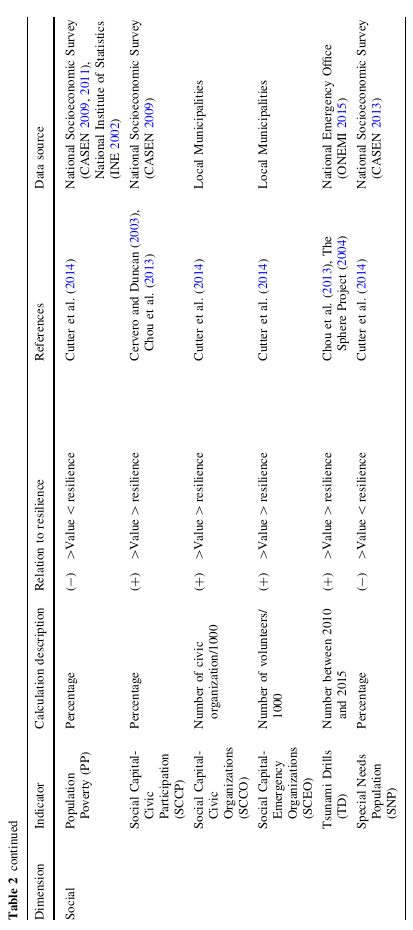
\includegraphics[width=0.55\textwidth]{img_07.png}
  \caption[Indicadores de la dimensi\'on social del modelo CORE]{Indicadores de la dimensi\'on social del modelo CORE. Fuente: \textcite{villagra2017}}
  \label{fig:indicadores-social}
\end{figure}


\chapter{Ejemplos de datos extra\'idos}
\label{app:datos}

Este anexo presenta un documento representativo de cada colecci\'on de MongoDB, tal como queda almacenado tras la ejecuci\'on del flujo ETL. Se omiten los campos que agrega Mongoose de forma autom\'atica (\texttt{\_id}, \texttt{\_\_v}, \texttt{createdAt} y \texttt{updatedAt}).

\section{Colecci\'on emergencia-desastres}
\label{app:datos-ed}

Cada documento corresponde a un simulacro. El campo \texttt{key} es la clave \'unica generada por el \textit{HashAdapter} a partir de la fecha y la regi\'on can\'onica, y es el mecanismo que impide almacenar un mismo simulacro dos veces.

\begin{lstlisting}[style=codigo, language=JSON]
{
  "key": "2021-05-27-arica-y-parinacota",
  "date": "2021-05-27T04:00:00.000Z",
  "place": "Sismo Tsunami - Sector Educación",
  "region": "Arica y Parinacota",
  "regionSource": "Arica",
  "indicator": "simulacros-2021",
  "module": "emergencia-desastres"
}
\end{lstlisting}

\section{Colecci\'on tasa-pobreza-ingresos}
\label{app:datos-pobreza}

La colecci\'on contiene una fila por unidad territorial. Los porcentajes se almacenan como n\'umeros, convertidos desde el formato decimal chileno que utiliza la fuente.

\begin{lstlisting}[style=codigo, language=JSON]
{
  "key": "comuna-de-valdivia-biblioteca-congreso-nacional-
           valdivia-tasa-pobreza-ingresos",
  "unidadTerritorial": "Comuna de Valdivia",
  "casen2017": 7.6,
  "casen2022": 3.4,
  "indicator": "valdivia-tasa-pobreza-ingresos",
  "module": "biblioteca-congreso-nacional"
}
\end{lstlisting}

\section{Colecci\'on organizaciones-comunitarias}
\label{app:datos-orgs}

Cada documento agrupa los 11 tipos de organizaci\'on comunitaria de un a\~no. El ejemplo corresponde al a\~no 2024 e ilustra el problema descrito en la secci\'on~\ref{sec:resultado-orgs}: los campos que la fuente no informa quedan almacenados como cero.

\begin{lstlisting}[style=codigo, language=JSON]
{
  "key": "0yhktp6",
  "anio": 2024,
  "nDeJuntasDeVecinos": 175,
  "nDeClubesDeportivos": 180,
  "nCentrosCulturales": 37,
  "nDeCentrosUOrganizacionesDelAdultoMayor": 92,
  "nDeCentrosDePadresYApoderados": 35,
  "nDeCompaniasDeBomberos": 10,
  "nDeUnionesComunales": 2,
  "nDeCentrosDeMadres": 0,
  "nDeOtrasOrganizacionesComunitariasFuncionalesOtros": 0,
  "nDeOrganizacionesComunitariasSumaTotal": 531,
  "indicator": "valdivia-organizaciones-comunitarias",
  "module": "biblioteca-congreso-nacional"
}
\end{lstlisting}

\section{Colecci\'on indicator-results}
\label{app:datos-results}

Esta colecci\'on almacena el valor del indicador calculado por el \textit{CalculatorAdapter}, separado de los registros crudos que le dieron origen.

\begin{lstlisting}[style=codigo, language=JSON]
{
  "indicator": "simulacros-2022",
  "module": "emergencia-desastres",
  "totalDrills": 11,
  "drillsByRegion": {
    "Arica y Parinacota": 1, "Tarapacá": 1, "Atacama": 1,
    "Valparaíso": 1, "O'Higgins": 1, "Maule": 1, "Ñuble": 1,
    "Biobío": 1, "Los Ríos": 1, "Aysén": 1, "Magallanes": 1
  }
}
\end{lstlisting}


\chapter{Declaraci\'on de un indicador}
\label{app:codigo}

Este anexo muestra el c\'odigo necesario para incorporar un indicador al sistema, con el objeto de dimensionar el esfuerzo real que implica esa tarea. Se utiliza como ejemplo el indicador \texttt{simulacros-2021} del m\'odulo \textit{emergencias-desastres}. El c\'odigo fuente completo del sistema se encuentra disponible en el repositorio del proyecto.

\section{Declaraci\'on mediante el IndicatorBuilder}
\label{app:codigo-config}

La declaraci\'on de un indicador consiste en encadenar los m\'etodos del \textit{IndicatorBuilder} indicando su nombre, la URL de la fuente, la frecuencia de actualizaci\'on y los \textit{adapters} que resuelven cada etapa del flujo ETL. El \textit{CalculatorAdapter} es opcional y solo se declara en los indicadores que requieren un valor agregado.

\begin{lstlisting}[style=codigo, language=TypeScript]
export const EMERGENCIA_DESASTRES_CONFIG: ModuleConfig = {
  "simulacros-2021": new IndicatorBuilder()
    .setName("Simulacros 2021")
    .setUrl("https://web.archive.org/web/20211026024955/...")
    .setFrequency(FREQUENCIES.once)
    .setFetchAdapter(new RequestPromiseAdapter())
    .setParseAdapter(new DateParserAdapter())
    .setMapperAdapter(new EmergenciaDesastresMapper())
    .setHashAdapter(new EmergenciaDesastresHashAdapter())
    .setStorageAdapter(new EmergenciasDesastresStorageAdapter())
    .setCalculatorAdapter(new TsunamiDrillsCalculatorAdapter())
    .build()
};
\end{lstlisting}

Los \textit{adapters} de obtenci\'on (\textit{RequestPromiseAdapter}) son gen\'ericos y se reutilizan entre indicadores; los restantes son espec\'ificos de la fuente.

\section{Extracci\'on de los datos desde el HTML}
\label{app:codigo-parse}

El \textit{ParseAdapter} concentra el conocimiento sobre la estructura de la fuente. Es la \'unica pieza que debe modificarse cuando una p\'agina cambia su HTML, y su aislamiento permite probarla sin ejecutar el resto del flujo.

\begin{lstlisting}[style=codigo, language=TypeScript]
export class DateParserAdapter implements ParseAdapter {
  extract(data: string) {
    const $ = cheerio.load(data);
    return $(".back-fechas .item .card")
      .map((_idx, elem) => {
        const dateElem = $(elem).find(".caja-date");
        const date = {
          day: Number($(dateElem).find(".dat_day")
                 .text().trim().split("\t")[0]),
          month: $(dateElem).find(".dat_mes").text().trim(),
          year: Number($(dateElem).find(".dat_year").text().trim())
        };
        const placeElem = $(elem).find(".card-body");
        const place = {
          type: $(placeElem).find(".card-title a").text().trim(),
          region: $(placeElem).find(".card-title.pb-3").text().trim()
        };
        return { date, place };
      })
      .get();
  }
}
\end{lstlisting}

\end{document}
